\documentclass[global,twocolumn]{svjour}
\journalname{SoSyM}

\usepackage{makeidx}
\pagestyle{headings}

\usepackage[final,pdftex]{graphicx}
        \pdfcompresslevel=9
        \DeclareGraphicsExtensions{.png}

\usepackage{chngcntr}

\usepackage{epsfig}
\usepackage{caption}  
\usepackage{subcaption} 
  
\captionsetup{compatibility=false}
 
\usepackage{calc}
\usepackage{amssymb}
\usepackage{amstext}
\usepackage{amsmath}
%\usepackage{multicol} 
\usepackage{pslatex} 
\usepackage{multirow}
\usepackage[table, dvipsnames]{xcolor}
\usepackage{color, colortbl}
\usepackage{algorithm}
\usepackage{algpseudocode} 
\usepackage{rotating}  
\usepackage{nzproof}
\usepackage{stmaryrd}

\usepackage[normalem]{ulem} % for \sout
\usepackage{xcolor}
\definecolor{colgray}{gray}{0.75}

% Put edit comments in a really ugly standout display
\usepackage{ifthen}
\usepackage{amssymb}
\newboolean{showcomments}
\setboolean{showcomments}{true} % toggle to show or hide comments
\ifthenelse{\boolean{showcomments}}
  {\newcommand{\nb}[2]{
    \fcolorbox{gray}{yellow}{\bfseries\sffamily\scriptsize#1}
    {$\blacktriangleright$#2$\blacktriangleleft$}
   }
   \newcommand{\version}{\emph{\scriptsize$-$working$-$}}
  }
  {\newcommand{\nb}[2]{}
   \newcommand{\version}{}
  }

%\newcommand\rs[1]{\nb{levi}{\textsl{#1}}}
%\newcommand\mf[1]{\nb{bernhard}{\textsl{#1}}}
%\newcommand\mc[1]{\nb{bentley}{\textsl{#1}}} 




\makeatletter
%\def\cl@chapter{\cl@chapter \@elt {theorem}}%bug in class
\def\cl@chapter{\@elt {theorem}}
\makeatother

\usepackage[capitalise,noabbrev]{cleveref} 

\usepackage{catchfilebetweentags}
\usepackage[section]{extraplaceins}

\definecolor{Gray}{gray}{0.9}
 
 \usepackage{setspace}
\onehalfspacing 

%\subfigtopskip=0pt
%\subfigcapskip=0pt
%\subfigbottomskip=0pt

\renewcommand\floatpagefraction{.9}
\renewcommand\topfraction{.9} 
\renewcommand\bottomfraction{.9}
\renewcommand\textfraction{.1}   
%\renewcommand{\baselinestretch}{1.5}
\setcounter{totalnumber}{50}
\setcounter{topnumber}{50}
\setcounter{bottomnumber}{50}
\setlength{\intextsep}{8pt} % Vertical space above & below [h] floats
\setlength{\textfloatsep}{8pt} % Vertical space below (above) [t] ([b]) floats
\setlength{\abovecaptionskip}{5pt}
\setlength{\belowcaptionskip}{5pt}

\newcommand{\chunk}[2]{% 
	\fcolorbox{black}{yellow}{\bfseries\sffamily\scriptsize#1}%
   {$\blacktriangleright$#2$\blacktriangleleft$}%
}
\newcommand{\bentley}[1]{\chunk{Bentley}{\textbf{\textcolor{ForestGreen}{\textsl{#1}}}}}
\newcommand{\levi}[1]{\chunk{Levi}{\textbf{\textcolor{red}{\textsl{#1}}}}}
\newcommand{\bernhard}[1]{\chunk{Bernhard}{\textbf{\textcolor{purple}{\textsl{#1}}}}}
\newcommand{\reviewer}[1]{\chunk{Reviewer}{\textbf{\textcolor{blue}{\textsl{#1}}}}}

\raggedbottom  

\usepackage{url}
\urldef{\maila}\path|{levi, hv}@cs.mcgill.ca, bentley.oakes@mail.mcgill.ca|

\begin{document}
%
%\mainmatter              % start of the contributions
%\  

\title{Symbolic Verification of Translation Model Transformations}  

 
\author{Levi \textsc{L\'ucio}\inst{1}\and Bentley James \textsc{Oakes}\inst{1}\and and Hans \textsc{Vangheluwe}\inst{2}\inst{1}}

\institute{School of Computer Science, McGill University, Canada\and
University of Antwerp, Belgium}

\maketitle              % typeset the title of the contribution  

\begin{abstract}

As model transformations are a required part of model-driven development, it is crucial to provide techniques that address their formal verification. One approach that has proven very successful in program verification is \emph{symbolic execution}. The symbolic abstraction in these techniques allows formal properties to be exhaustively proved for all executions of a given program.
In our approach we apply the same abstraction principle to verify model transformations. Our algorithm builds a finite set of path conditions which represents all concrete transformation executions through a formal abstraction relation. We are then able to prove properties over all transformation executions in a model-independent way. This is done by examining if any created path condition violates a given property, which will produce a counterexample if the property does not hold for the transformation. We demonstrate that this property proving approach is both valid and complete. Implementation results are also presented here which suggest that our approach is feasible and can scale to real-world transformations. 

\end{abstract}

\begin{keywords}
Model Transformations, Symbolic Verification, Translation 
\end{keywords}

% \begin{abstract}
% In the work we present in this paper we apply the \emph{program verification}
% concept of \emph{symbolic execution} to the verification of model
% transformations written in the Turing-incomplete DSLTrans language. Our symbolic
% execution construction algorithms leverage on DSLTrans' reduced expressiveness
% in order to cope with the classical state space explosion problem typical to
% exhaustive verification techniques. By producing a symbolic execution for a
% DSLTrans model transformation we are able to prove precondition-postcondition
% axioms that regard the syntactic structure of our input/output models. Our
% property proofs are model independent, meaning a proof holds for any input model
% that satisfies an axiom's precondition. We are also able to produce a
% counterexample if a property does not hold. A counterexample consists of a set
% of transformation rules that, when executed, lead to the property being violated.
% 
% We have used model transformation technology to build the prototype we have used
% in the experiments with out technique we report in this paper. Metamodels and
% model transformations are used not only to produce the intermediate models we
% use for symbolic execution construction, but also at the core of our prototype
% in the symbolic execution construction algorithms. 
% \end{abstract}

% In this paper we present a novel technique and a prototype implementation for
% proving properties of model transformations expressed in the DSLTrans language.
% The approach is based on symbolic execution and the properties we are interested
% in concern relations between the structure of the input and output models. In
% particular, the properties are implications of the form `if a structural
% relation between some elements of the source model holds, then another
% structural relation between some elements of the target model must also hold'.
% Our technique is transformation dependent but model independent, meaning the
% proofs we produce hold for all executions of a given DSLTrans transformation 
% specification running on any instance of the transformation's input metamodel.
%  
% Our proof technique is based on (i) building the finite symbolic execution for a
% given DSLTrans transformation and (ii) on checking whether the property holds
% for all elements of the finite symbolic execution execution set. We explain how 
% a symbolic execution and a proof is built with our technique by using model
% transformations written using our T-Core framework.
\section{\uppercase{Introduction}}
\label{sec:intro}

Model transformations were described as the \emph{heart and soul} of model driven
software development (MDD) by Sendall and Kozaczynski in
2003~\cite{Sendall2003}.  Due to their practicality and appropriate level of
abstraction, model transformations are the current technique for performing
computations on models. In their well-known 2006 paper `A Taxonomy of Model
Transformations', the authors Mens, Czarnecki and Van Gorp call for the
development of verification, validation and testing techniques for model
transformations~\cite{Mens2006125}. Despite the many publications on this topic
since then, the field of analysis of model transformations seems to be still in
its (late) infancy, as evidenced by Amrani, L\'ucio \emph{et al.}~\cite{DBLP:conf/icst/AmraniLSCDVTC12}.

% Since then, many model transformation languages have emerged and are being
% used intensively not only in MDD, but also in other scopes, such as when
% software development processes benefit from formalised translators between
% languages.

In this paper, we present our work on verification of properties on model
transformations. Specifically, we discuss concrete algorithms that can prove
whether properties will hold or do not hold on all executions of a
transformation written in the DSLTrans transformation language. Properties are
proved through a process that constructs a set of path conditions, where
each path condition symbolically represents an infinite number of concrete transformation
executions through an \emph{abstraction relation}.

% The technique has been extended from its original presentation
% in~\cite{Lucio:10}, ~\cite{DBLP:conf/sle/BarrocaLAFS10}, and~\cite{LucVan:13}.

In our previous work~\cite{Lucio:10}, this property-proving algorithm was
presented as a proof-of-concept. In the present work, we significantly expand
that proof-of-concept by clarifying and offering discussions on validity and
completeness for the presented algorithms. We also provide an implementation
that we believe will scale to industrial applications, as validated by an
automotive case study~\cite{gehan:13}.
 


Our approach is feasible due to the use of the transformation language DSLTrans~\cite{DBLP:conf/sle/BarrocaLAFS10}. DSLTrans is
\emph{Turing incomplete}, as it avoids constructs which imply unbounded
recursion or non-determinism. Despite this \emph{expressiveness reduction}, we have shown via several
examples~\cite{febavava:10,dsltrans_manual,zhang:ACP_APN:11} that DSLTrans is
sufficiently expressive to tackle typical translation problems. This sacrifice
of Turing-completeness allows us to construct a\\provably-finite set of path
conditions~\cite{Lucio:10}. Our approach currently considers a core subset
of the DSLTrans language that does not include negative conditions in rules or attribute manipulation. These features of the language will be addressed in future work.

Informed by the structure of DSLTrans transformations, our approach defines an algorithm for the creation of path conditions. Each path condition that is created represents a set of concrete
transformation executions through an \emph{abstraction relation} that we formally define. Once the set of all path conditions has been created for the transformation, we can then prove structural \emph{model syntax
relations}~\cite{DBLP:conf/icst/AmraniLSCDVTC12} using this relation. Such properties are essentially pre-condition/post-condition axioms involving statements about whether certain elements of the input model have been correctly transformed into elements of the output model, and have been explored by several authors~\cite{Akehurst:02,Narayanan:07,DBLP:journals/eceasst/CariouBBD09,DBLP:journals/ase/GuerraLWKKRSS13}.
In our proof technique, the properties examined can be proven to hold for all executions of a given
model transformation, no matter the input model.
Therefore, our technique is \emph{transformation dependent} and \emph{input
independent}~\cite{DBLP:conf/icst/AmraniLSCDVTC12}.

Our methods differ from previous work in the transformation verification field
in that we require no intermediate representation for a specific proving
framework (as in~\cite{ButtnerEC12,ButtnerECG12,DBLP:conf/icst/AsztalosLL10}) but instead work on DSLTrans
transformations themselves. Along with DSLTrans rules, all of the constructs
involved in our algorithms are typed graphs. This intuitive representation allows
our property proving technique to be composed of relatively simple steps, as the
metamodels, models, and properties involved are all constructed using a similar
graphical representation.

% This also provided us with performance gains over our
% previous implementation, due to the use of efficient graph-matching libraries to manipulate the graph structures required.

A large difficulty in any exhaustive proof technique is the tendency for the
state space to explode, even when abstractions are performed to render the
search space finite.  A later section of this work will discuss optimisation
opportunities and performance results obtained from our implementation. The
scalability of our approach will also be analysed in order to infer the
algorithm's potential applicability to real-world problems. A real-world industrial case study will also be briefly presented.

Our specific contributions include:

\begin{itemize}
\item An algorithm for constructing all path conditions for a given DSLTrans transformation;
\item An algorithm that proves transformation properties over these path conditions;
\item Validity and completeness proofs of the path condition construction and property proving algorithms;
\item A discussion of performance and scalability results for our implementation.
\end{itemize}

This paper is organised as follows: \cref{sec:dsltrans} briefly introduces
the DSLTrans model transformation language and its formal semantics, while the formal background for this work is presented in \cref{sec:formal_background}. The algorithms to build the complete set of path
conditions for the transformation will be discussed in
\cref{sec:building_pcs}. \cref{sec:abstraction_relation} will present the abstraction relation found in our technique, along with examples, while \cref{sec:verif_dsltrans_props} will examine how this abstraction relation is used in our process for proving properties. In \cref{sec:implementation} and \cref{sec:experiments}, we introduce our implementation with sample scalability results; \cref{sec:related_work} presents the related work;
and finally in \cref{sec:conclusion} we conclude with remarks and future
work.
 
\section{The DSLTrans Transformation Language}
\label{sec:dsltrans}

In this section we will introduce the DSLTrans transformation language and its
constructs from~\cite{DBLP:conf/sle/BarrocaLAFS10}. A formal treatment of the syntax and semantics of DSLTrans is found in \cref{sec:DSLTrans_formal_appendix}.

\reviewer{Please explain, earlier on, the meaning of indirect edges.}


\begin{figure*}[t]
        \centering
        \begin{subfigure}[b]{0.40\textwidth}
                \centering
                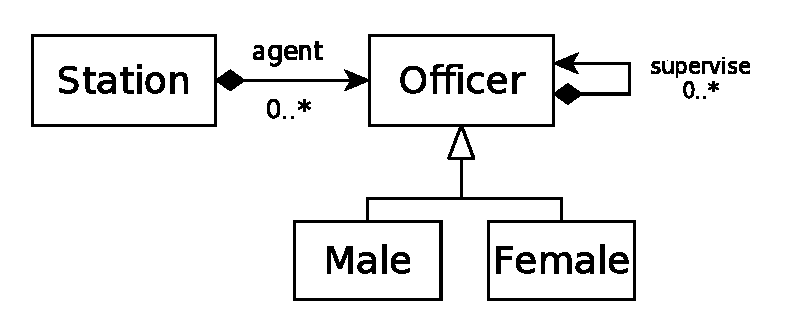
\includegraphics[width=1\textwidth]{./figures/policestation_dsltrans/organization.pdf}
                \caption{Organization language}
                \label{fig:OrganizationLanguage}
        \end{subfigure}%
        ~~
        \begin{subfigure}[b]{0.40\textwidth}
                \centering
                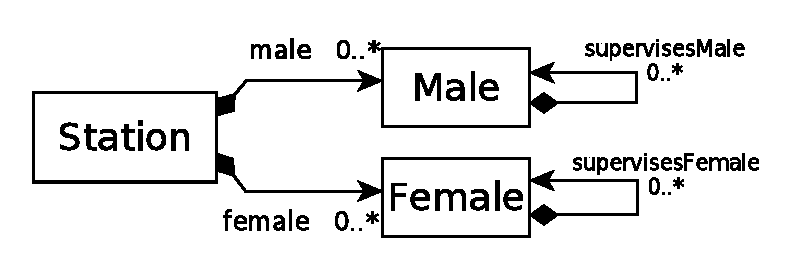
\includegraphics[width=1\textwidth]{./figures/policestation_dsltrans/gender.pdf}
                \caption{Gender language}
                \label{fig:GenderLanguage}
        \end{subfigure}%
        \caption{Metamodels for the Police Station transformation}
        \label{fig:squadmetamodel}
\end{figure*}

A DSLTrans transformation has a source and a target metamodel, which are seen
in \cref{fig:squadmetamodel}. This \emph{Police Station}
transformation will be presented throughout
the rest of this paper as an example transformation. The metamodel
in \cref{fig:OrganizationLanguage} represents a language for describing
the chain of command in a police station, which includes the male (\emph{Male}
class) and female officers (\emph{Female} class). The metamodel in
\cref{fig:GenderLanguage} represents a language for describing a different
view over the chain of command, where the officers working at the police station
are classified by gender.

\begin{figure*}[bht]
	\centering
		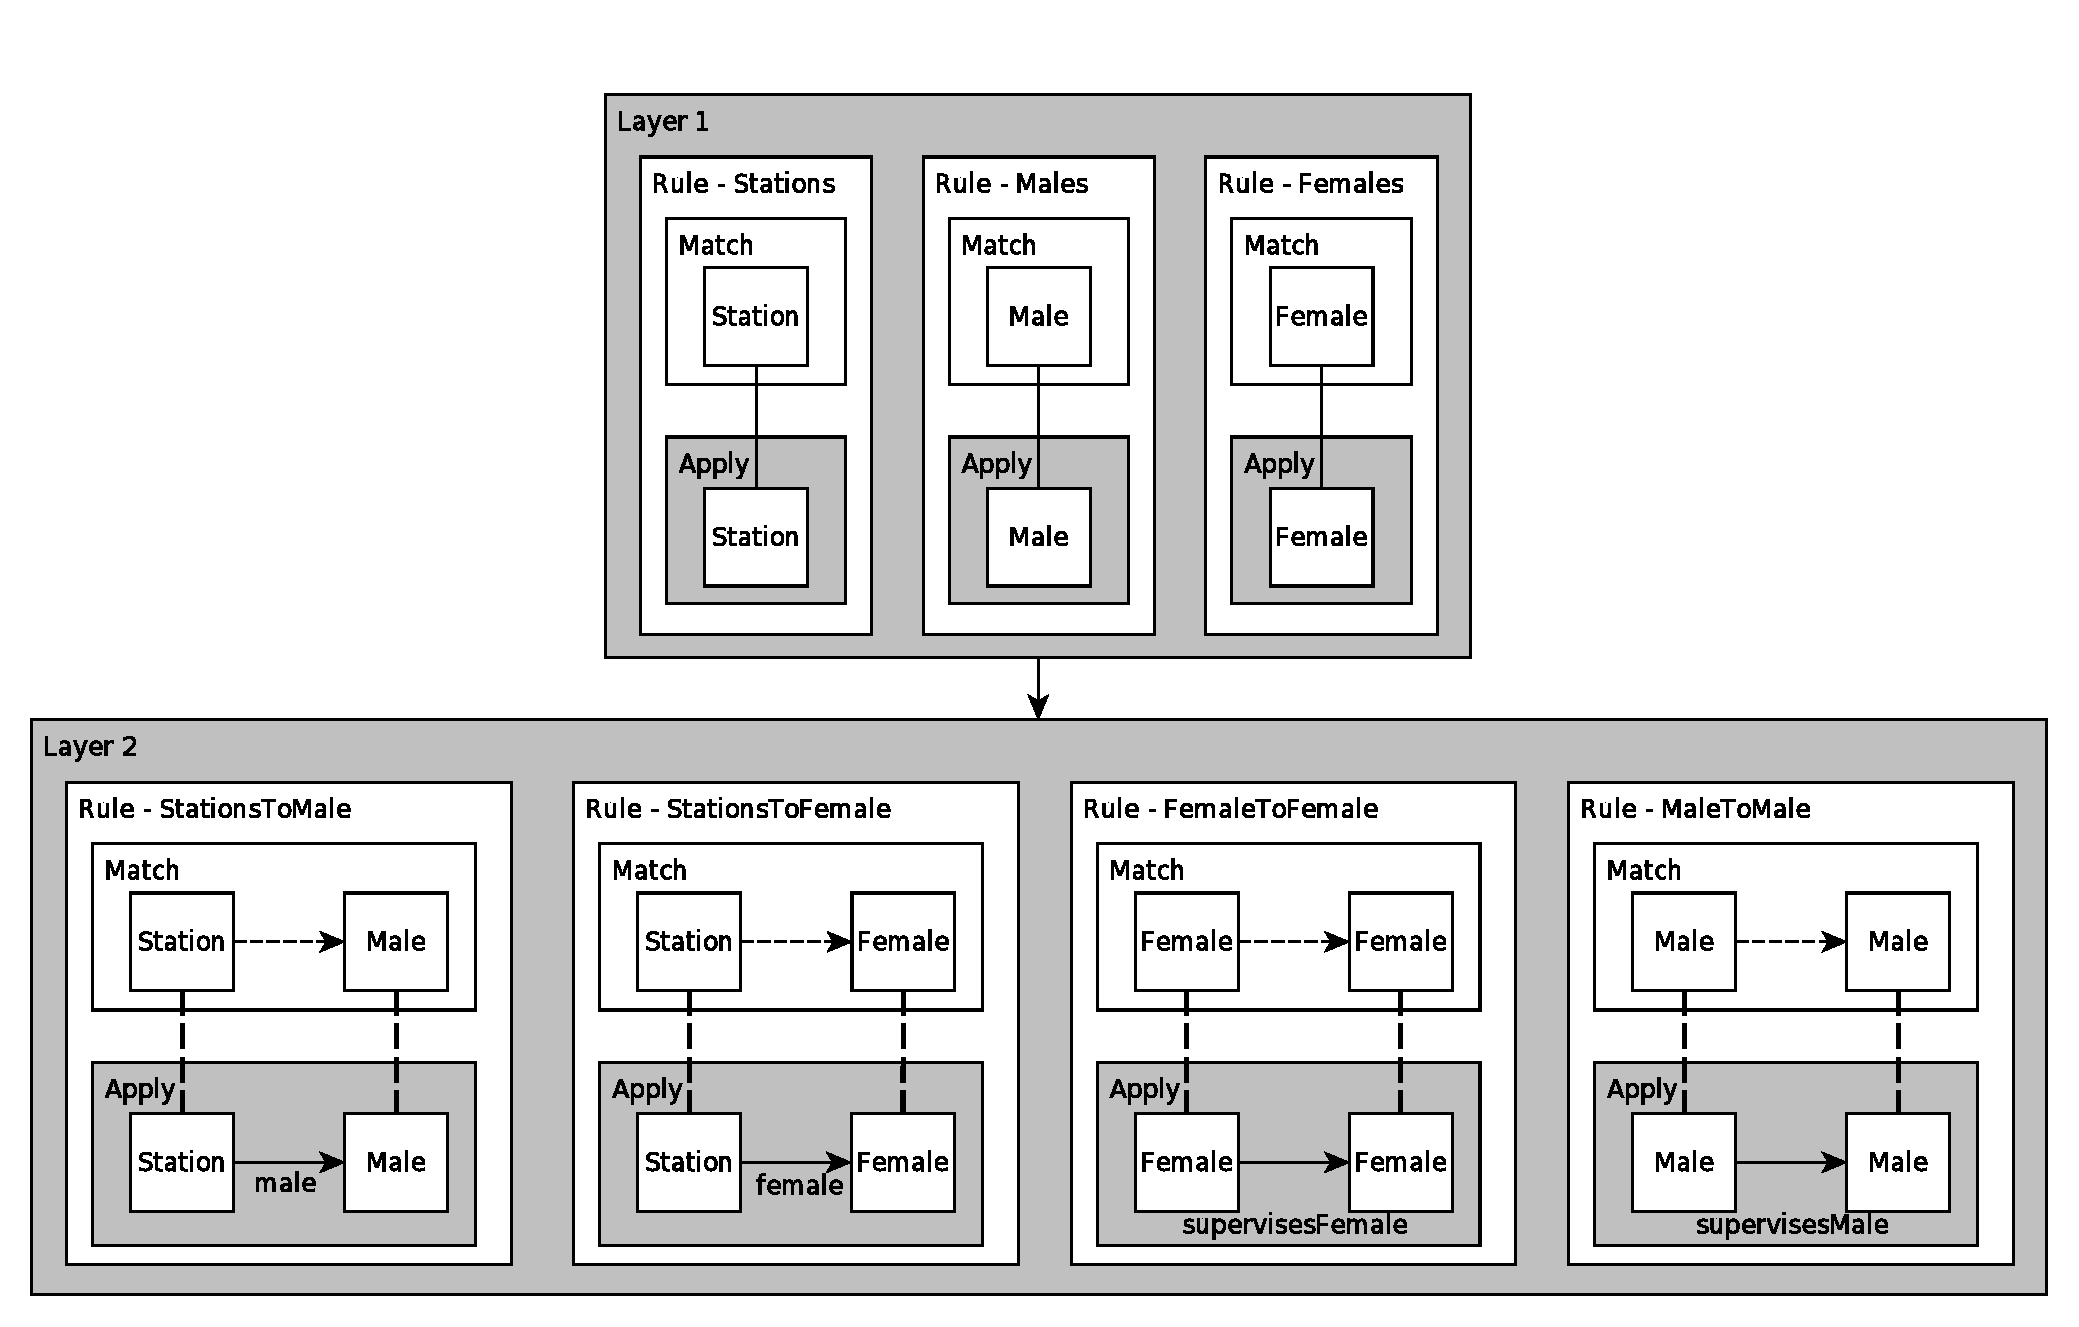
\includegraphics[width=0.9\textwidth]{./figures/policestation_dsltrans/transformation.pdf}
	\caption{The \emph{Police Station} model transformation expressed in DSLTrans}
	\label{fig:dsltransformation}
\end{figure*}

In \cref{fig:dsltransformation} we present a DSLTrans transformation that involves both metamodels.  A description of relevant constructs as well as visual notation remarks are found in \cref{subsec:DSLTrans_constructs}. Note
that the transformation is formed
from layers where each layer is a set of transformation rules. The
transformation will execute layer-by-layer, where transformation rules in a layer will execute in a
non-deterministic order but will always produce a deterministic result, due to the fact that DSLTrans is confluent by construction~\cite{DBLP:conf/sle/BarrocaLAFS10}.

Another important characteristic of DSLTrans transformations is that they are not Turing-complete. As discussed in~\cite{DBLP:conf/sle/BarrocaLAFS10}, non-completeness is required to make a transformation execution always terminate, but yet still allows for appropriate expressiveness.

Besides the fact that DSLTrans' transformations are free of constructs that
imply unbounded recursion or \\non-determinism, DSLTrans' transformations are strictly outplace, meaning no changes are allowed to the input model. However, the output metamodel for a DSLTrans transformation can
be the same as the input metamodel. Also, elements cannot be removed
from the output metamodel as the result of applying a DSLTrans rule.
This restriction is consistent with the usage of model transformations as
translations~\cite{AMT2012}, as no deletion of output elements is strictly required.

The purpose of this \emph{Police Station} transformation is to flatten a chain of command given
in the \emph{Organization language} into two independent sets of male
and female officers represented in the \emph{Gender language}. The command
relations will be kept during this transformation, i.e. a female officer will
have a direct association to all her female subordinates and likewise for male
officers. Note that differences in the gender classification metamodel mean
some relations present in the input model will not be retained in the output
model.

\begin{figure*}[htb]
        \centering
        \begin{subfigure}[b]{0.30\textwidth}
                \centering
                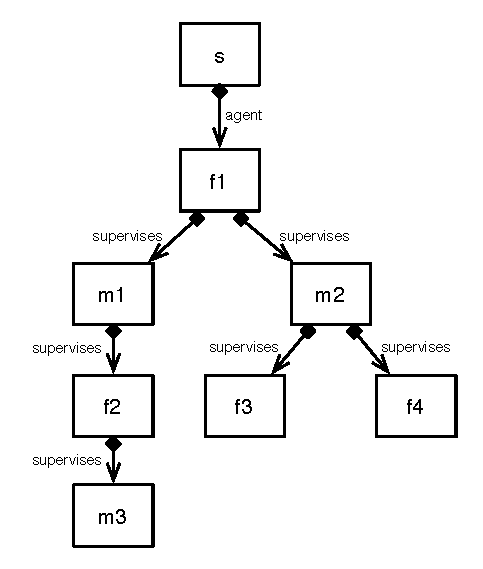
\includegraphics[width=1\textwidth]{./figures/policestation_dsltrans/model_police_hierarchy.pdf}
                \caption{Original model}
                \label{fig:police_hierarchy}
        \end{subfigure}%
        ~~
        \begin{subfigure}[b]{0.40\textwidth}
                \centering
                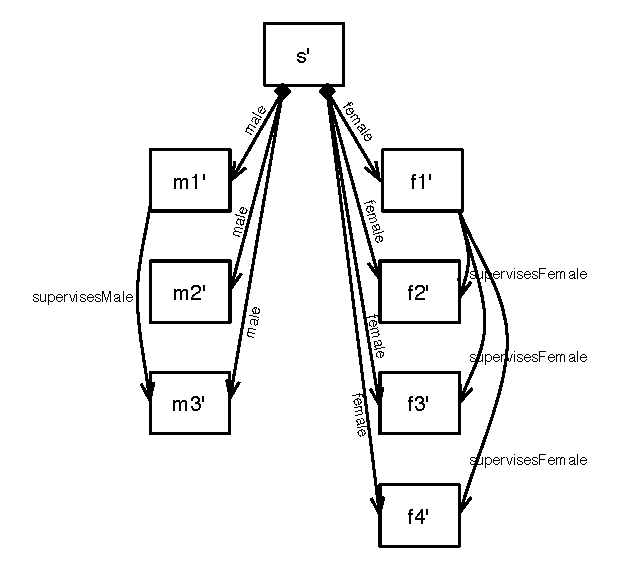
\includegraphics[width=1\textwidth]{./figures/policestation_dsltrans/model_police_gender.pdf}
                \caption{Transformed model}
                \label{fig:police_gender}
        \end{subfigure}%
        \caption{Model before and after transformation}
        \label{fig:transformationexample}
\end{figure*}
\reviewer{Figure 3: I would suggest adding another node f5 superviesd by f4, to illustrate the
notion of transitive closure. Another remark: I think the black containment dia-
monds do not belong in an instance model, as they are a metamodel notion.}

An example of this transformation's execution can be observed in \cref{fig:transformationexample}, where the input model is on the left and the output model is on the right. Notice that the elements $s$, $m_k$  and $f_k$ in \cref{fig:OrganizationLanguage} are instances of the source \emph{Organization} metamodel elements $Station$, $Male$ and $Female$ respectively. The primed elements in \cref{fig:police_gender} are their counterpart instances in the target \emph{Gender} metamodel.

Each individual transformation rule in the transformation is composed of two graphs. The first graph
is denoted as the \emph{match graph}, and is a pattern holding elements from the
source metamodel. Likewise, the \emph{apply graph} is a pattern containing
elements from the target metamodel. A formal definition of a transformation rule is found in~\cref{def:transformation_rule} in \cref{sec:formal_background}.

As an example, consider the transformation rule marked \emph{Stations} in the
first rule layer in \cref{fig:dsltransformation}. The match graph holds
one \emph{Station} element from the source metamodel, while the apply graph
holds one \emph{Station} element from the target metamodel. This means that for all
elements in the input model which are of type \emph{Station} in the
\emph{Organization Language}, an element of type
\emph{Station} in the \emph{Gender Language} will be created in the output model.

Note that in our approach, we require that the match graph of a rule is not a subgraph of the match graph of any other rule (as formally stated in \cref{def:layer_transformation} of model transformation, in \cref{sec:formal_background} of this paper). This requirement is to prevent the case where a rule could not execute independently of another rule, except for the cases when such dependency is explicitly defined by backward links. This is undesirable for the algorithm as presented here as we will explain later. However, as seen in~\cite{conf/gg/SelimLCDO14}, the expressiveness of the transformations our algorithm can examine \reviewer{Perhaps 'the expressiveness of the rule language'?}  is not restricted. In that work, we detail an operational rule processing step to handle overlapping rules.

\reviewer{In page 10 (answer to the reviewers) you say that rules for a 
  layer must be parallel independent. Is this written anywhere in the
  main part of the paper? }

\subsection{Properties to Prove}

The properties we aim to prove on the Police Station transformation are structural properties. These properties are composed of a pre-condition and a post-condition component, as seen in \cref{fig:properties}. 

Informally, a property can be read as `if the pre-condition graph matches on the input model to the transformation, then the post-condition graph will match any output model produced'. Further details as well as formal validity and completeness of the property proving process are discussed in \cref{sec:verif_dsltrans_props}.

As a brief example of property syntax and semantics, consider the property in \cref{fig:dsltrans_prop1}. The pre-condition graph is composed of a Station element connected to a Female element and a Male element, where all elements are from the \emph{Organization language} metamodel. This structure is repeated in the post-condition graph, with the difference that the metamodel for these elements is the \emph{Gender language}. Thus, this property represents the statement ``\emph{a model which includes a
police station that has both male and female officers will be
transformed into a model where the male officer will exist in the male set
and the female officer will exist in the female set}''. We expect this property to always hold in our transformation.

\begin{figure*}[thb]
        \centering
        \begin{subfigure}[b]{0.45\textwidth}
                \centering
                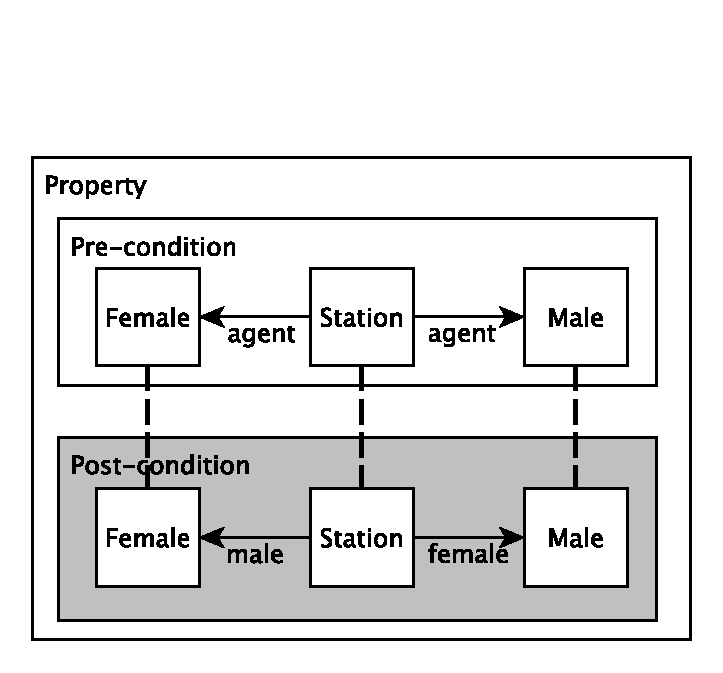
\includegraphics[height=5.5cm]{./figures/policestation_dsltrans/property1.pdf}
                \caption{Property 1 -- Expected to hold}
                \label{fig:dsltrans_prop1}
        \end{subfigure}%
        ~~
        \begin{subfigure}[b]{0.45\textwidth}
                \centering
                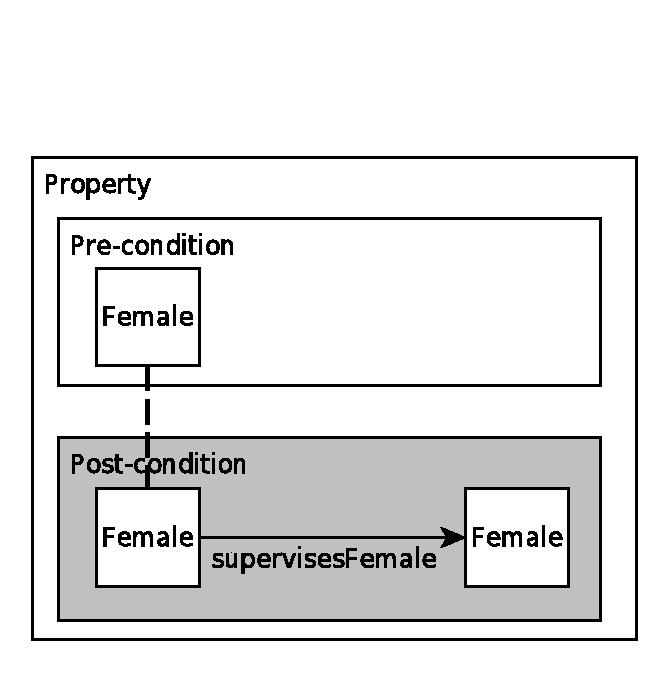
\includegraphics[height=5.5cm]{./figures/policestation_dsltrans/property2.pdf}
                \caption{Property 2 -- Not expected to hold}
                \label{fig:dsltrans_prop2}
        \end{subfigure}%
        \caption{ Properties to be proved on the Police Station transformation}
        \label{fig:properties}
\end{figure*}

\reviewer{Figure 4: The two “agent” edges in the postcondition should be marked “female”
resp. “male”} 
In contrast, we do not expect the property in \cref{fig:dsltrans_prop2} to always hold. This property represents the statement ``\emph{any model which includes a
female officer will be transformed into a model where that female officer will
always supervise another female officer}''. It is not difficult to construct an input model where the pre-condition holds, but the post-condition does not. For example, take an input model that contains only one female officer, as there will only be one female officer in the output model.

We shall discuss our property proving technique in \cref{sec:verif_dsltrans_props}. Following this, experiments in \cref{sec:experiments} will present experimental results from proving these two properties on the Police Station transformation.





\subsection{DSLTrans Constructs}
\label{subsec:DSLTrans_constructs}
This section will describe all of the DSLTrans constructs involved in our
property-proving algorithm. These constructs are found in the transformation presented in \cref{fig:dsltransformation}. Formal details for the handled constructs are found in \cref{sec:DSLTrans_formal} and \cref{sec:DSLTrans_syntax}, while \cref{sec:DSLTrans_semantics} briefly introduces the formal semantics of this subset of DSLTrans. The visual syntax presented here is based on the DSLTrans Eclipse plug-in syntax~\cite{dsltrans_manual}.

\begin{itemize}
\item \textbf{Match Elements}: Match elements are variables typed by elements of the source
metamodel which will match over elements of that type (or subtype) in the
input model when the transformation is executed. Note that match
elements in a rule are searched for injectively in a model. This means that, for
example, if a match graph includes two elements of type \emph{Station}, then the rule will only match over models that include at least two instances of type \emph{Station}.

In the DSLTrans notation as seen throughout this paper, the match elements will be in a white box in the top half of a rule.\\

\item \textbf{Direct Match Links}: Direct match links are variables typed by labelled associations of the source metamodel, which will match over associations of the same type in the input model. A direct match link is always expressed between two match elements.\\

\item \textbf{Indirect Match Links}: Indirect match links are similar to direct
match links, but there may exist a path of containment associations between the
matched instances. Our notion of indirect links captures only
acyclic EMF containment associations. \reviewer{“a nonempty path” (I think). The label of the
containment associations does not matter?}

% As such, it avoids cycles and infinite
% amounts of matches over the transitive closure of associations in the input
% models.

In \cref{fig:dsltransformation}, indirect match links are represented in all the
transformation rules in the last layer as dashed arrows between elements in the match graph.\\

\item \textbf{Backward Links}: Backward links connect elements of the match and
the apply patterns of a DSLTrans rule in order to represent dependencies on
element creation by previous layers of the transformation. When used in a rule,
backward links match over traceability links between elements of the
transformation's input and output models.
These traceability links are implicitly created when any rule is executed during the transformation. Backward
links thus make it possible to refer in a rule to output elements created by a
previous layer.

Backward links are found in \cref{fig:dsltransformation} in all transformation rules on the last layer and are depicted as dashed lines.\\

%\item \emph{Negative Conditions}: it is possible to express negative conditions over
%match elements, backward, direct and indirect match links. 

\item \textbf{Apply Elements and Apply Links}: Apply elements and apply links are similar to match elements and
match links, but are instead typed by elements of the target metamodel. Apply elements in a given transformation rule that are not connected to backward links will create elements of the same type in the transformation's output. Apply links will always be created in the transformation's output. These output elements and links will be created as many times as the match graph of the rule is isomorphically found in the input model.\\

Consider the transformation rule denoted \emph{Station2Male} in the last rule
layer of \cref{fig:dsltransformation}. This rule takes \emph{Station} and
\emph{Male} elements of the \emph{Gender Language} metamodel, where these
elements were created in a previous layer from \emph{Station} and \emph{Male}
elements of the \emph{Organization Language} metamodel, and connects them using a
\emph{male} association.

%\item \emph{Apply Attributes}: DSLTrans includes a small language for
%building the values attributes of apply model elements from references to one or
%more match model element attributes.
\end{itemize}



\section{Formal Background}
\label{sec:formal_background}

In this section we will introduce the formal concepts that will be used throughout all this paper. We start in \cref{sec:typed_graphs} by a few (typed) graph concepts that will be used as mathematical building blocks throughout this paper. In particular we will introduce the notion of typed graph, typed graph union and subset, and useful relations between typed graphs based on homomorphisms. Notice that these concepts are well known from graph theory and are only slightly customized for our purposes.

\reviewer{Your formalisation is made more complex than necessary because you do not put
the power of typed graphs to work. If your source and target metamodels have
disjoint types (which you can assume without loss of generality) you can take
their union, augmented with trace edge types from all target node types to all
source node types, and take that to be the meta-model for an input-output model,
and also for a rule. Suddenly you don’t have to carry arround the distinction be-
tween Match and Apply (for rules) or input and output (for input-output models)
around any more: they are just the projections onto the types of the source, resp.
target metamodel.}

\reviewer{Section 4.2.2 on “backward links” is rather confusing, as it speaks about trace-
ability links being added to rules. You never add traceability links to rules any-
where in the paper; in fact, your formal notion of a rule has no room for them.
Instead, rules only have backward links. (The clarity of the the situation is not
improved by the fact that those are labelled trace.)}

\reviewer{I think the situation would be much more clear if you were to use the common
notion of left hand side and right hand side of a rule. The left hand side of a
rule rl is precisely your ||rl||, the right hand side is the entire rl augmented by
your traceability links, as in 4.2.2. Suddenly we are back in a well-known graph
transformation formalism, and your rules are in fact so simple (no deletion, no
negative application conditions, injective matching) that I believe it makes no
difference whether you use algebraic graph transformation or some more con-
structively defined variant. The only standard notion is that of transitive closure
in the left hand side; but there are plenty of GT tools that offer this extension.
In fact I see no reason why your rule application would then not precisely coin-
cide with the the same notion in, say, SPO graph rewriting; and I hope you agree
that this would help you no end in explaining what you are doing. (If, on the
other hand, there is after all some difference then this, too, would be interesting
to know, as that difference is not at all apparent right now.)}

\reviewer{Viewed like this, moreover, I think your notions of input-output models and rules
are very close to triple graph transformation as used by Schrr at all. I think the
main (if not only) difference lies in the fact that your "glue graph" is actually not
a graph; instead, you use traceability edges directly from the target model to the
source model. If you were to turn those edges into nodes with source and target
edges, even that difference would disappear.}


Armed with the fundamental notion of typed graph, we can then introduce other formal concepts in Sections~\ref{sec:DSLTrans_formal}, \ref{sec:DSLTrans_syntax} and \ref{sec:DSLTrans_semantics} which describe the artifacts from the modeling and transformation world that we require for our verification technique. Naturally, we start by introducing the central notion of \emph{metamodel}, allowing the description of the inputs and outputs of a model transformation. Other fundamental notions we will define in this section are \emph{model}, \emph{transformation rule}, \emph{transformation} and the semantic concept of \emph{model transformation execution}. Several auxiliary and intermediate notions for defining the syntax and semantics of our techniques will also be introduced here. 

Note that this section presents a collection of formal tools that are used in the subsequent sections of this paper where the contributions of this paper are presented. It is meant as a formal reference for the upcoming formal development. %This section can be safely skipped or skimmed by the reader, who can return to these definitions punctually to understand the detailed formal underpinning of our approach. 

\reviewer{There is a lot of redundancy in the paper, on several levels:
  - input-output-models, path conditions and properties are
    all defined very similarly. Couldn't you subsume them in a single
    definition and spell out the differences?}


\newcommand{\defineggprime}{Let $\langle V,E,(s,t),\tau,VT,ET\rangle = g$, and\\ $\langle V',E',(s',t'),\tau',VT',ET'\rangle = g'$, where $g, g' \in \textsc{TG}$.}

\newcommand{\ET}{\mathit{ET}}
\newcommand{\VT}{\mathit{VT}}


\bentley{Make sure that terminology is consistent between elements and vertices}

\subsection{Graph Structures and Functions}
\label{sec:typed_graphs}


\subsubsection*{Typed Graph}
We will start by introducing the notion of typed graph. A typed graph is the essential object we will use throughout our mathematical development. Typed graphs will be used to formalise all the important graph-like structures we will present in this paper. A typed graph is a directed multigraph (a graph allowing multiple edges between two vertices) where vertices and edges are typed.


\begin{definition}{Typed Graph\\}
\label{def:typed_graph}
A typed graph is a 6-tuple $\langle V,E,(s,t),\tau, \VT, \ET\rangle$ where:
\begin{itemize}
\item $V$ is a finite set of vertices
\item $E$ is a finite set of directed edges connecting the vertices $V$
\item $(s,t)$ is a pair of functions $s: E\rightarrow V$ and $t: E\rightarrow V$ that respectively provide the source and target vertices for each edge in the graph
\item Function $\tau:V\cup E\rightarrow \VT \cup \ET$ is a typing function for the elements of $V$ and $E$, where $\VT$ and $\ET$ are disjoint finite sets of vertex and edge type identifiers and $\tau(v)\in \VT$ if $v\in V$ and $\tau(e)\in \ET$ if $e\in E$
\item Edges $e\in E$ are noted $v\xrightarrow{e} v'$ if $s(e)=v$ and $t(e)=v'$, or simply e if the context is unambiguous
\item The set of all typed graphs is called $\textsc{TG}$
\item We define the empty graph to be a graph with $V = \emptyset$, $E = \emptyset$, and the other elements to be empty functions
\end{itemize}
\end{definition}


\subsubsection{Vertex and Edge Types}

Note that the our verification technique is geared toward model-driven engineering. Therefore, the types of vertices and edges in our typed graphs will be drawn from a particular \textit{metamodel}.

Sample metamodels for our running example can be seen in figures above \bentley{Fix.}. The particular metamodel for a typed graph will be indicated in the formalization when required, as (potentially) different metamodels will be present for the input and output graphs in DSLTrans rules.

We assume the existence of a number of functions in our formalization to aid the treatment of typing:

\begin{itemize}
\item $\mathit{isAbstract}: \mathit{VT} \rightarrow \{\mathit{true}, \mathit{false}\}$
\begin{itemize}
\item Where $\mathit{isAbstract}(\VT)$ returns $\mathit{true}$ iff $\VT$ is denoted as abstract (not able to be instantiated) by the metamodel, else $\mathit{false}$
\end{itemize}

\item $\mathit{isIndirect}: \mathit{ET} \rightarrow \{\mathit{true}, \mathit{false}\}$
\begin{itemize}
\item Where $\mathit{isIndirect}(\ET)$ returns $\mathit{true}$ iff $\ET$ is denoted as an \textit{indirect edge}, else $\mathit{false}$. The \textit{indirect} classification allows matching over indirect paths between vertices. This will be further clarified when required for our constructs.
\end{itemize}

\item $\mathit{matchesOver}: \{\VT \cup \ET\} \times \{\VT \cup \ET\} \rightarrow \{\mathit{true}, \mathit{false}\}$

\begin{itemize}
\item The purpose of this function is to assist in handling polymorphism in the metamodel
\item $\mathit{matchesOver}(T, T) \rightarrow \mathit{true}$
\item $\mathit{matchesOver}(T, T') \rightarrow \mathit{true}$ iff T' is a subclass of T in some defined partial ordering $\leq$ given by the metamodel
\item Otherwise, $\mathit{false}$
\end{itemize}
\end{itemize}

For simplification purposes, we will not represent edge cardinalities or containment relationships given by a metamodel in our notion of typed graph. Note that in fact we require these conditions to be relaxed to perform our graph rewriting.

\subsubsection*{Typed Subgraph}
We now define the useful notion of typed subgraph. As expected, a typed subgraph is simply a restriction of a typed graph to some of its vertices and edges. 

\begin{definition}{Typed Subgraph\\}
\label{def:typedsubgraph}
\defineggprime

$g'$ is a typed subgraph of $g$, written $g'\sqsubseteq g$, iff $V'\subseteq V$, $E'\subseteq E$ and $\tau'=\tau |_{V'\cup E'}$.

\end{definition}

Given a typed graph $g\in \textsc{TG}$, will use the notation $Components(g)$ to describe the set of strongly connected typed graphs in $g$. Also, we will use the notation $g|_{t}$ to refer to the restriction of graph $g$ to its subgraph containing only edges of type $t$.


\subsubsection*{Typed Graph Union}
We now define how two typed graphs are united. A union of two typed graphs is trivially the set union of all the components of those two typed graphs. Note that we do not require the components of the two graphs to be disjoint, as in the following joint unions will be used to merge typed graphs.

\begin{definition}{Typed Graph Union\\}
\label{def:typed_graph_union}

The typed graph union is the function $\sqcup :\textsc{TG}\times \textsc{TG}\rightarrow \textsc{TG}$ defined as:
\begin{multline*}
\big\langle V,E,(s,t),\tau,\VT,\ET\big\rangle\;\sqcup\;\big\langle V',E',(s',t'),\tau',\VT',\ET'\big\rangle=\\
\big\langle V\cup V', E\cup E',(s\cup s', t\cup t'), \tau\cup \tau', \VT\cup \VT', \ET\cup ET'\big\rangle
\end{multline*}
\end{definition}

Note: as a reviewer helpfully pointed out, we require that $s \cup s'$, $t \cup t'$, and $\tau \cup \tau'$ coincide on common elements. However, this can be assumed w. l. o. g..


\bentley{Do we need typed graph intersection? Or to mention what it means for two graphs to be disjoint?}

\subsubsection*{Typed Graph Homomorphism}
For the formal development of our technique, we are interested in relations between typed graphs that are structure-preserving, i.e. homomorphisms. Homomorphisms between typed graphs preserve not only structure, but also the types of vertices and edges that are mapped. Note that, trivially, a typed graph homomorphism is a graph homomorphism.

\begin{definition}{Typed Graph Homomorphism\\}
\label{def:typed_graph_homomorphism}
\defineggprime

A typed graph homomorphism between $g$ and $g'$ is a function $f: f_v \cup f_e$ such that:
\begin{itemize}
\item $f_v: V\rightarrow V'$
\item $f_e: E\rightarrow E'$
\item $\forall v_1 \xrightarrow{e} v_2\in E$:
\begin{itemize}
\item Let $ v_1' = f_v(v_1), v_2' = f_v(v_2), e' = f_e(e)$
\item $v_1', v_2' \in V', e' \in E'$
\item $s'(e') = v_1'$, $t'(e') = v_2'$
\item $\mathit{matchesOver}(\tau(v_1), \tau(v_1') \land \\\mathit{matchesOver}(\tau(v_2), \tau(v_2') \land\\ \mathit{matchesOver}(\tau(e), \tau(e')$
\end{itemize}

%, where $\tau(v_1)=\tau'(f(v_1))$, $\tau(v_2)=\tau'(f(v_2))$ and also $\tau(e)=\tau(e')$.
\item The domain of $f$ is noted $Dom(f)$ and the co-domain of $f$ is noted $CoDom(f)$.
\end{itemize}  
\end{definition}

\bentley{Maybe put `inj' and `sub' in the homomorphism to reduce number of symbols}
 When an \emph{injective} typed graph homomorphism $f$ exists between $g$ and $g'$ we write $g \stackrel{f}{\vartriangleleft} g'$, or simply $g \vartriangleleft g'$ when the context is unambiguous. When a \emph{surjective} typed graph homomorphism $f$ exists between typed graphs $g$ and $g'$ we write $g \stackrel{f}{\blacktriangleleft} g'$, or also simply $g \blacktriangleleft g'$ in an unambiguous context. 

\subsubsection*{Typed Graph Edge Homomorphism}

Our technique also requires a form of graph homomorphism that primarily focuses on matching the edges of the graphs. This homomorphism will be an injective match regarding the edges, but note that a particular vertex in the source graph may match onto multiple vertices in the target graph. \bentley{What's the term for this?}

\begin{definition}{Typed Graph Edge Homomorphism\\}
\label{def:typed_graph_edge_homomorphism}
\defineggprime

A typed graph edge homomorphism between $g$ and $g'$ is a function $h: h_v \cup h_e$ such that:
\begin{itemize}
\item $h_v: V'\rightarrow V$
\begin{itemize}
\item Note that $h_v$ is an function from a vertex in the target graph onto a vertex in the source graph
\end{itemize}
\item $h_e: E\rightarrow E'$
\item $\forall v_1 \xrightarrow{e} v_2\in E$:
\begin{itemize}
\item Let $e' = h_e(e), v_1' = s'(e'), v_2' = t'(e')$
\item $v_1', v_2' \in V', e' \in E'$
\item $v_1 = h_v(v_1'), v_2 = h_v(v_2')$
\item $\mathit{matchesOver}(\tau(v_1), \tau(v_1') \land \\\mathit{matchesOver}(\tau(v_2), \tau(v_2') \land\\ \mathit{matchesOver}(\tau(e), \tau(e')$
\end{itemize}

\end{itemize}  
\end{definition}

Again, we wish to highlight the fact that this homomorphism is different than Definition~\ref{def:typed_graph_homomorphism} in the vertex matching function. A vertex in the target graph matches onto a vertex in the source graph, with multiple target vertices matching onto the same source vertex. 
\bentley{Create diagram to illustrate}

This unusual homomorphism allows our technique to `split' our source graph over multiple locations in the target graph. This is critical, as our target graphs are constructed in a way that allows for vertex duplication. That is, two vertices of a particular type in the target graph may only represent one underlying element, as discussed in Section~\ref{sec:abstraction_relation}. Constructing this morphism allows our prover implementation to avoid explicitly creating `disambiguated' graphs where these duplications are resolved.


\subsection*{Typed Graph Isomorphism}
Two typed graphs are said to be isomorphic if they have exactly the same shape and related vertices and edges have the same type.


\begin{definition}{Typed Graph Isomorphism\\}
\label{def:typed_graph_isomorphism}
\defineggprime

We say that $g$ and $g'$ are isomorphic, written $g\cong g'$, iff there exists a bijective typed graph homomorphism $f:V\rightarrow V'$ such that $f^{-1}:V'\rightarrow V$ is a typed graph homomorphism.
\end{definition}




\subsubsection*{Transitive Closure}

DSLTrans matching constructs allow for the matching of indirect links, where as described in Section~\ref{subsec:DSLTrans_constructs}, rules may match over indirect paths between elements. This transitive closure allow for the explicit creation of all edges implied by these indirect links to aid in matching.


\begin{definition}{Transitive Closure\\}
\label{def:instance_closure}

Let $g$ be a graph $\langle V,E,(s, t),\tau\rangle \in \textsc{TG}$. Then the transitive closure $g^{*} = \langle V,E',(s, t),\tau\rangle \in \textsc{TG}$, where:

$E' = E \cup $ the transitive closure of $\big\{v\xrightarrow{e}v' | \mathit{isIndirect(e)} \big\}$
\end{definition}


Given a graph, its transitive closure includes, besides the original graph, all the edges belonging to the transitive closure of indirect links in that graph. Note that these transitive edges are given by the function $\mathit{isIndirect}$.

\bentley{I believe that the indirect edges don't need to be removed. There's a bit of handwaving, so maybe there are edge duplicates?}

In the definitions that follow we will use the $*$ notation, as in \cref{def:instance_closure}, to denote the transitive closure of our structures.


\subsection{DSLTrans Constructs}
\label{sec:DSLTrans_formal}



This section will detail the abstract syntax of the constructs involved in a DSLTrans transformation.

As discussed in Section~\ref{subsec:DSLTrans_syntax}, DSLTrans transformations are composed of rules arranged in layers.


\subsubsection*{DSLTrans Transformation Rule}

A transformation rule is the elemental block of a DSLTrans transformation. Several transformation rules can be observed in the Police Station transformation in \cref{fig:dsltransformation}.

A transformation rule includes a non-empty match pattern and a non-empty apply pattern. This is also known in the model transformation literature as a rule's \emph{left hand side} and \emph{right hand side}. A match pattern can include indirect links that are used to transitively match containment relations in a model. The apply pattern of a rule always contains at least one apply element that is not connected to a backward link or an edge, meaning in practice that a rule will always produce something and not only match. An apply pattern does not include indirect links as it is used only for the construction of parts of instances of a metamodel.

A rule may also contain a negative application condition (NAC) which if matched over the source graph prevents application of the rule.

A transformation rule also includes backward links, as informally introduced in \cref{subsec:DSLTrans_constructs}. As described in that section, backward links define dependencies between rules. \bentley{Expand}


\begin{definition}{DSLTrans Transformation Rule\\}
\label{def:transformation_rule}

A DSLTrans transformation rule is a four-tuple $\big\langle \mathit{NAC}$, $\mathit{Match}$, $\mathit{Apply}$, $\mathit{backward}\big\rangle$, where:

\begin{itemize}
\item $\mathit{NAC}$, $\mathit{Match}, \mathit{Apply} \in \textsc{TG}$
\item $\mathit{Match}$ and $\mathit{Apply} $ are non-empty and are disjoint
\item $\mathit{NAC}$ may be an empty graph, and is disjoint from both $\mathit{Match}$ and $\mathit{Apply} $
\item $\mathit{backward} = \{E_{back}, (s_{back}, t_{back})\}$
\end{itemize}  

Note that when we require an element of the $\mathit{Match}$, $\mathit{Apply}$, or $\mathit{NAC}$ graphs, such as the vertices, we will index the required element. For example, the vertices for the \textit{Match} graph will be $V_{\textit{Match}}$.

\begin{itemize}
\item $E_{back}$ contains the backward links
\begin{itemize}
\item $E_{back} $ is disjoint from $E_{Match}$,  $E_{Apply}$, and $E_{NAC}$
\end{itemize}
\item $(s_{back}, t_{back})$ is a pair of functions $s_{back}: E_{back}\rightarrow V_{\textit{Apply}}$ and $t_{back}: E_{back}\rightarrow V_{\textit{Match}}$ that respectively provide the source and target vertices for each backward link
\begin{itemize}
\item Note the source of backward links is a vertex in $V_{\textit{Match}}$ while the target is a vertex in $V_{\textit{Apply}}$
\end{itemize}
\end{itemize}

\textsc{Rules} is the set of all rules.

\end{definition}

We additionally impose that for the well-formedness of a DSLTrans rule, there always exists an element or edge to be created in the \textit{Apply} graph to be created. That is, either there are edges to be created in the \textit{Apply} graph, or there is a vertex in the \textit{Apply} graph that is not the source of a backward link.

\begin{itemize}
\item $E_{\textit{Apply}} \neq \emptyset \lor$
\item $ \exists v \in V_{\textit{Apply}} | \big\{\forall e \in E_{back}: s_{back}(e) \neq v \big\}$
\end{itemize}



\subsubsection*{DSLTrans Layer and Transformation}

\cref{def:layer} and \cref{def:transformation} formalise the abstract syntax of a model transformation, introduced in \cref{sec:dsltrans}. An example of a model transformation can be observed in \cref{fig:dsltransformation}, the Police Station transformation. As expected, a DSLTrans transformation is composed of a sequence of layers where each layer is composed of a set of rules.

\begin{definition}{Layer\\}
\label{def:layer}
A layer is a finite set of transformation rules: $\{r_0, r_1, \dots, r_n | r_i \in \textsc{Rules}\}$.

The set of all layers is denoted $\textsc{Layers}$. 
\end{definition}

Note that the order of the rules within the layer does not matter, due to the semantics of DSLTrans rule execution.

\begin{definition}{DSLTrans Transformation\\}
\label{def:transformation}

A DSLTrans transformation is a finite list of layers denoted $\{l_0, l_1, \dots, l_n | l \in \textsc{Layers}\}$. Note that the order of layers in a transformation is important.

The set of all transformations is denoted $\textsc{Transforms}$.



\end{definition}



\subsubsection*{Input-Output Model}

To describe the semantics of a DSLTrans model transformation, we must define an \textit{input-output model} construct. This input-output model allows the representation of intermediate operational states during the execution of a model transformation.

The structure of a input-output model is intentionally very similar to a DSLTrans rule. There is one typed graph representing the input model and another typed graph representing the output model. As well, the construct contains a set of edges, named \emph{traceability links}, for keeping a history of which elements in the output model originated from which elements in the input model.

\begin{definition}{Input-Output Model\\}
\label{def:input_output_model}

An input-output model rule is a three-tuple $\big\langle \mathit{Input}$, $\mathit{Output}$, $\mathit{trace}\big\rangle$, where:

\begin{itemize}
\item $\mathit{Input}, \mathit{Output} \in \textsc{TG}$
\item $\mathit{Input}$ and $\mathit{Output} $ may be empty and are disjoint
\item $\mathit{trace} = \{E_{trace}, (s_{trace}, t_{trace})\}$
\begin{itemize}
\item $E_{trace}$ contains the traceability links
\item $E_{trace} $ is disjoint from $E_{Input}$ and $E_{Output}$
\item $(s_{trace}, t_{trace})$ is a pair of functions $s_{trace}: E_{trace}\rightarrow V_{\textit{Output}}$ and $t_{trace}: E_{trace}\rightarrow V_{\textit{Input}}$ that respectively provide the source and target vertices for each traceability link
\end{itemize}

\end{itemize}  

Let $\mathit{IOM}$ be the set of all input-output models.

We define a utility function getTransformation: IOM $\rightarrow$ Transforms. This function returns the Transform that the input-output model was built for. The purpose of this function is to restrict input-output models to only be applicable for the transformation they represent.

Note that the $\VT$ and $\ET$ for input and output will come from the input and output metamodels. \bentley{Expand} 

\bentley{Do we need to have V and E for all vertices and edges in the IOM? I don't think we talk about all vertices or edges in an IOM.}
Additionally we have that $V=V'\cup V''$, $E\subseteq E'\cup E''$ and $\tau\subseteq \tau'\cup \tau''$, where the co-domain of $\tau$ is the union of the co-domains of $\tau'$ and $\tau''$ and the set $\{trace\}$.

\end{definition}


\subsection{Transformation Semantics}
\label{sec:DSLTrans_semantics}

This section will discuss the semantics of a DSLTrans transformation. Given an input model and a transformation, an output layer will be produced through the repeated execution of rules and layers.




\subsubsection*{Execution of a DSLTrans Rule}

We will now address the execution of a rule in the DSLTrans language. 

We will base our explanation on double pushouts, diagrammed in Figure~\ref{fig:dpo}.
\bentley{Single or double pushouts?}

\begin{figure}[h!] \centering
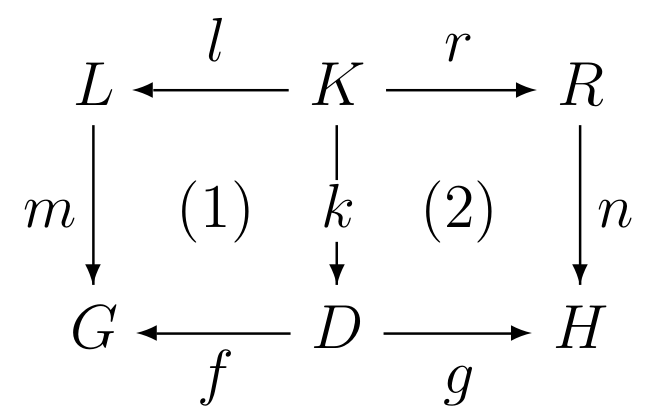
\includegraphics[width=0.44\textwidth]{figures/formal/dpo}
	\caption{Double pushout approach}
	\label{fig:dpo}
\end{figure}

We explain the components:
\begin{itemize}
\item L: The matcher of the rule
\item R: The rewriter of the rule
\item G: The graph to be matched/rewritten
\item H: The rewritten graph
\end{itemize}

Note that as it is not possible in DSLTrans rules to remove elements, $L = K$, and $G = D$.


\subsubsection*{Matcher of a Transformation Rule}

To create the actual matcher construct that will be matched during a rule's execution, the rule's \textit{Match} graph is combined with backward links, as well as any \textit{Apply} vertices connected to the backward links.

Note that the rule's NAC will also be considered in the matching of a rule.

\begin{definition}{Matcher of a Transformation Rule\\}
\label{def:matcher_transformation_rule}

Let the transformation rule $r = \big\langle \mathit{NAC}$, $\mathit{Match}$, $\mathit{Apply}$, $\mathit{backward}\big\rangle$.

Let $\mathit{Match}\star$ be the transitive closure of $\mathit{Match}$ to handle any indirect edges.

\bentley{Typed graph? Or copy the rule's structure? If it is a rule, note that it will not be well-formed. However, this is preferable to defining another structure to use}

We define $r$'s matcher, noted $\lceil r \rceil$, to be a typed graph six-tuple $\langle V,E,(s,t),\tau, \VT, \ET\rangle$, where:
\begin{itemize}
\item $V = V_{Match\star} \cup \big\{v \in V_{Apply} | \{\exists e \in E_{back} | s_{back}(e) = v\}\big\}$
\item $E = E_{Match\star} \cup E_{back}$
\item $s = s_{Match\star} \cup s_{back}$, $t = t_{Match\star} \cup t_{back}$
\item $\tau = \tau_{Match\star} \cup \tau_{Apply}$
\item $\VT = \VT_{Match\star} \cup \VT_{Apply}$
\item $\ET = \ET_{Match\star} \cup \ET_{Apply}$
\end{itemize}

\end{definition}

\subsubsection*{Rewriter of a Transformation Rule}

To continue with the double pushout approach, we must construct the rewriting (or replacement) graph.

The construction of this rewriter is essentially the same as the underlying rule. However, to support traceability, we require that backward links in the rule be converted into traceability links, and that new traceability links be created between all match and apply vertices. 

\begin{definition}{Rewriter of a Transformation Rule\\}
\label{def:rewriter_transformation_rule}

Let the transformation rule $r = \big\langle \mathit{NAC}$, $\mathit{Match}$, $\mathit{Apply}$, $\mathit{backward}\big\rangle$.

Let $\mathit{Match}\star$ be the transitive closure of $\mathit{Match}$ to handle any indirect edges.

We define $r$'s rewriter, noted $\lfloor r \rfloor$, to be a input-output model $\big\langle \mathit{Input}$, $\mathit{Output}$, $\mathit{trace}\big\rangle$, where:

\begin{itemize}
\item $ \mathit{Input} = \mathit{Match\star}$
\item $ \mathit{Output} = \mathit{Apply}$
\end{itemize}

We then modify $\mathit{trace}$ to contain the appropriate traceability links

\begin{itemize}
\item $E_{trace} = E_{backward} \cup \big\{e | \{$for each pair $m_i, a_j$ where $m_i \in V_{Match}, a_j \in V_{Apply}\}\big\}$
\item $s_{trace} = s_{backward} \cup \big\{a_j | \{$for each pair $m_i, a_j$ where $m_i \in V_{Match}, a_j \in V_{Apply}\}\big\}$
\item $t_{trace} = t_{backward} \cup \big\{m_i | \{$for each pair $m_i, a_j$ where $m_i \in V_{Match}, a_j \in V_{Apply}\}\big\}$
\end{itemize}

\bentley{Very messy}
\end{definition}

\subsubsection*{Application of a Transformation Rule (continued)}

\bentley{Fix up morphism notation. Is $\rightarrow$ good enough?} 
Recall that the interface graph K is equivalent to L due to the lack of deletion in DSLTrans rules. Thus, the l homomorphism is identity. The D correspondence graph will therefore be equivalent to G.


As well, we consider r to be a trivial homomorphism between the $\mathit{Match} \rightarrow \mathit{Input}$, $\mathit{Apply} \rightarrow \mathit{Output}$, and $\mathit{backward} \rightarrow \mathit{trace}$.

We also note here that a rule cannot be applied if there is a homomorphism between the rule's NAC and G. 

m is the typed graph homomorphism between the matcher of a rule $r$, denoted ($\lceil r \rceil$) and the $\mathit{Input}$ component of the input-output model

$n$ and $g$ will be homomorphism between their respective graphs. \bentley{This needs to be explained further. Maybe with a diagram?}

\subsubsection*{DSLTrans Layer Execution}

Now that the application of a particular DSLTrans rule has been explained, the next definition defines how a DSLTrans transformation layer executes. Recall that a layer is composed of rules, and acts on the current input-output model.


\begin{definition} {DSLTrans Layer Execution}
\label{def:dsltrans_layer_execution}


The execution of a DSLTrans layer can be defined as a function as follows:

\textit{applyLayer} : IOM $\times$ Layer $\rightarrow$ IOM

Let $l = \{r_0, r_1, \dots, r_n | r_i \in \textsc{Rules}\}$, $l \in \textsc{Layers}$.

Let $\mathit{IOM}_{Input}$, $\mathit{IOM}_{Output} \in \mathit{IOMs}$.

$\mathit{IOM}_{Output}$ will be the result of applying the production \textit{p} as defined below to $\mathit{IOM}_{Input}.$

We refer to the double-pushout literature for the creation of \textit{p}. Specifically, we refer to the definition of parallel direct derivations. This p will be created out of the productions created for each of the rules $r_i$ in the layer.

$p = \big\langle (p_1, {in}^1), \dots, (p_k, {in}^k) \big\rangle : (L \xleftarrow{l} L \xrightarrow{r} R)$

This collection of the rules is possible because DSLTrans rules do not delete anything. Essentially, a union is taken of the L, K, R components of each production.
\end{definition}

\begin{figure}[h!] \centering
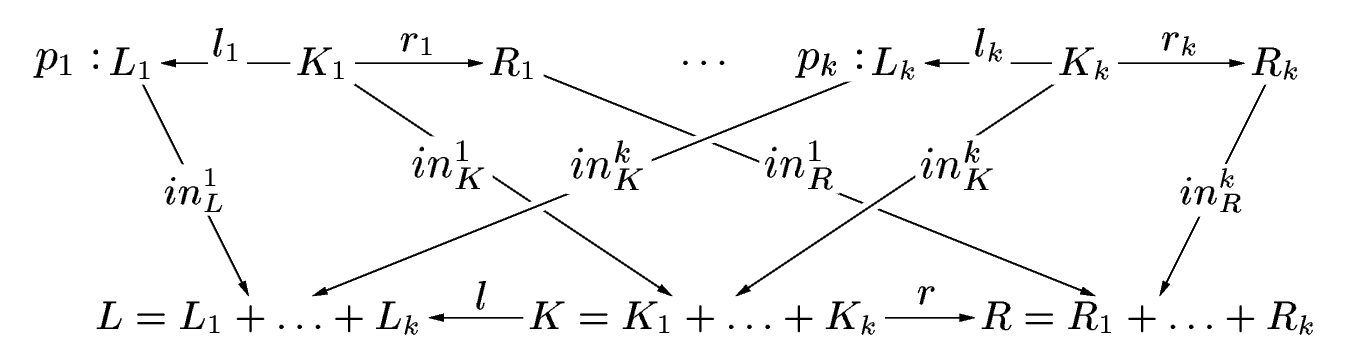
\includegraphics[width=0.44\textwidth]{figures/formal/parallel_productions}
	\caption{Parallel production \textit{p}}
	\label{fig:parallel_productions}
\end{figure}


\cref{def:dsltrans_layer_execution} is the core of DSLTrans' semantics, in which we build the result of executing a layer of a DSLTrans transformation. Many model transformation languages are based on graph rewriting, where the result of each rule rewrite is immediately usable by all other rules. In DSLTrans the result of executing one layer in DSLTrans is totally produced before the input to the layer is changed. This is enforced in \cref{def:dsltrans_layer_execution} by the fact that the layer production is composed of a union of the rule's productions. Rules belonging to the same layer are thus forced to execute independently, as described in the section on DSLTrans semantics.

\bentley{How does this handle different multiplicity of rule application?}


\subsubsection*{DSLTrans Transformation Execution}

Our final definition is for the execution of a DSLTrans transformation. Essentially, it is the chaining of layer executions applied on an input-output model.

We will begin by discussing the conditions for executing a model transformation on an input model.


\paragraph{Input Conditions}

For a well-formed transformation execution, we require the \textit{input-output model} in the domain to contain only an input graph. Recall that an \textit{input-output model} is the three-tuple $\big\langle \mathit{Input}$, $\mathit{Output}$, $\mathit{trace}\big\rangle$. We therefore require that both the $\mathit{Output}$ and $\mathit{trace}$ components in the domain IOM to be empty. This input-output model thus represents the first step of the transformation, where no rule has been executed yet.

The input-output model in the co-domain will contain this input graph, as well as the output graph and traceability links produced by the execution of the transformation. Let $\textsc{Execs}_t$ be the set of all well-formed input-output models produced for transformation $t$.

\begin{definition} {Execution of a DSLTrans Transformation\\}
\label{def:DSLTrans_transformation_execution} 

The execution of a model transformation is a function $\mathit{applyTransformation}: \mathit{IOM} \times \mathit{Transforms} \rightarrow \mathit{IOM}$.

This function is a chaining of executions of those layers within the transformation.

Recall the application of a layer is \textit{applyLayer} : IOM $\times$ Layer $\rightarrow$ IOM. Therefore, the application of a transformation is:

$\mathit{IOM}$ as input to chaining of layer executions \bentley{Is this function chaining? I don't know how to write the equation for this.}


\end{definition}


While the execution of the rules belonging to a layer happens in parallel, the execution of the layers of a transformation happens sequentially. As per \cref{def:DSLTrans_transformation_execution}, the input-output model that is the output of executing a given layer is passed onto the next layer as input. The final input-output model created will be the result of the model transformation.



\subsection{Confluence and Termination Properties}

We now prove two important properties about executions of transformations expressed in the subset of DSLTrans presented in this paper: \emph{confluence} and \emph{termination}. The proofs are provided at a high level, given the fact that DSLTrans essentially enforces both these properties by construction of the semantics of DSLTrans.

\begin{proposition}{Confluence}

Every model transformation execution is confluent up to typed graph isomorphism.

\bentley{As we are relying on the double-pushout approach, I think we get this confluence for free.}


\end{proposition}

\begin{pf}
We want to prove that for every model transformation execution of a transformation $\mathit{transform} \in \textsc{Transforms}$ having as input an input-output model $\mathit{input} \in \mathit{IOMs}$, its output is always the same up to typed graph isomorphism.\\


If we assume an execution of the transformation is not confluent then this should happen because of non-determinism when the execution of a transformation is being built. Non-determinism happens during the construction of a transformation execution at two points: 
\begin{enumerate}
\item The section `Execution of a DSLTrans Rule' discusses the matching and rewriting components to rule application. Note that our technique relies on the double-pushout approach, which itself is non-deterministic up to typed graph isomorphism, which does not contradict the proposition we are trying to prove. \bentley{Revise this.}


\item In Definition~\ref{def:dsltrans_layer_execution}, the rules composing a transformation layer are composed into a production on the input graph. Note that the order in which the transformation rules are composed may be non-deterministic. However, as these rules can be shown to be parallel independent \bentley{And they have to in that definition}, the production is by definition confluent up to typed graph isomorphism.

\end{enumerate}
Given there are no other sources of non-determinism when building the execution of a transformation, every model transformation execution is confluent up to typed graph isomorphism.
\end{pf}

\begin{proposition}{Termination}

Every model transformation execution terminates.
\end{proposition}
\begin{pf}
Let us assume that there is a transformation execution which does not terminate. In order for this to happen there must exist a part in the construction of the execution of a transformation which induces an algorithm with an infinite amount of steps. We identify three moments when this can happen:
\begin{enumerate}

\item If the matching and rewriting process of a rule is infinite. However, as the double-pushout approach uses a single production, then this must be a finite process. \bentley{Verify this, especially in the case of multiple applications of the rule.}

% if the result of the $match_{rl}(m_{in})$ function in definition~\ref{def:match_function} is an infinite set of match-apply graphs. The input-output model $m_{in}$ is by definition finite and the matching of each rule is independent from the execution of other rules in the same layer. As such, the number of subgraphs of $m_{in}$ isomorphic to $rl$'s matcher found during the execution of $rl$ is finite.


\item if Definition~\ref{def:dsltrans_layer_execution} of execution of a layer induces an infinite amount of steps. The only possibility for this to happen is if a layer has an infinite amount of transformation rules, which is a contradiction with Definition~\ref{def:layer}.

\item if Definition~\ref{def:DSLTrans_transformation_execution} of execution of a transformation induces an infinite amount of steps. Given layers are executed sequentially and no looping is allowed, the only possibility for this to happen is if the transformation has an infinite amount of layers, which contradicts Definition~\ref{def:transformation}.


\end{enumerate}
Given there are no other constructs in the semantics of a transformation that can induce an infinite amount of steps, every model transformation execution terminates.
\end{pf}



\section{Abstraction Relation between Path Conditions and Transformation Executions}
\label{sec:abstraction_relation}


% More informally, there exists a typed graph injective homomorphism between
% $Match_{pc}$ and $Input_x$  \textbf{and} $\langle V_x,E_x\setminus
% E_{mx},\tau_x\rangle$ is a typed graph strict instance of $\langle
% V_{pc},E_{pc}\setminus E_{pc},\tau_{pc}\rangle$.

% \levi{It is possible that this relation is required to be a typed graph strict
% instance between the path condition and the execution. Such a constraint would
% oblige each set of executions for a path condition to be truly distinct from
% the set of executions for another path condition. With the current definition
% the executions for a path condition including rule 'A' will overlap with the
% executions for a path condition including rules 'AB'. If this is so validity
% needs to be proved again for the new relation between the match patterns of PC
% and ex. Elements that do not show up in the match part of the rules are
% excluded from the typed graph strict instance.}



In this section we define the abstraction relation between the execution of a
DSLTrans transformation and the path condition that represents it.
This abstraction relation allows us to prove properties on a finite set of representative
path conditions, as created by the path condition generation algorithm. As this set is finite, our technique is  guaranteed to be decidable.

This section also presents our arguments that our path condition building
algorithm is both \emph{valid} and \emph{complete}. In this context
\emph{validity} means that for each path condition there exists at least one
transformation execution that it abstracts.
In other words, no path conditions are produced that lack a concrete
transformation execution counterpart. \emph{Completeness} of the symbolic
execution means that every transformation execution is abstracted by at least
one path condition.

Let us start by formally defining the notion of abstraction of a transformation
execution by a path condition.

\setcounter{equation}{0} 

\begin{definition}{Abstraction of a Transformation Execution by a Path Condition\\}
\label{def:abstraction_pc_ex}
\CatchFileBetweenTags{\abstractionrel}{text/definitions}{abstractionrel}{\abstractionrel}
\end{definition} 


% \cref{def:abstraction_pc_ex} enforces the fact that the matcher part of
% components of the path condition are found through an injective typed graph
% homomorphism in the execution's input model. Additionally, the graph including
% the output of the execution (including traceability information), can be
% mapped by a surjective typed graph homomorphism onto the apply model (plus the
% symbolic traceability links) of the path condition.

To understand the abstraction relation in \cref{def:abstraction_pc_ex}, recall
that during the construction of a transformation execution rules are matched
injectively in the input model. This information is present in the first
condition of the abstraction relation (Proposition~\ref{eq:abstr_input_output})
via the injective typed graph homomorphism between the match part of the copies
of rules ``glued'' onto the path condition and the containment transitive
closure of the input part of the transformation execution. This relation
enforces the fact that certain parts of the execution were found, or matched, by
certain parts of the path condition.
On the other hand, the surjection from the output of the execution towards the
apply part of the path condition models the fact that the output of the
execution has been completely built by instantiating the apply parts of the
rules contained in the path condition.

The second condition of the abstraction relation
(Proposition~\ref{eq:abstr_trace}) checks for the fact that symbolic
traceability links in the path condition and traceability links in the execution
correctly correspond to each other. This is modeled by the fact that all
strongly connected components in the path condition, composed only of symbolic
traceability links, are injectively found on the execution. This injection
models the fact that traceability graphs between individual or combined rules in
the path condition are necessarily found in the execution. Note that components
of the path condition are considered because of the fact that disconnected rules
in the path condition may have matched over common elements of a particular
execution. As such, a full injection between the complete traceability graph in
the path condition and the execution would be incorrect. Additionally, in the
second part of Proposition~\ref{eq:abstr_trace} we check the fact that every
traceability link in the execution can be found in the path condition. This
additional sanity check enforces that no spurious traceability links that could
not have been created by the rules present in the path condition exist in the
transformation execution.

%Finally, the last clause of the abstraction relation states that rule copies
%that are repeated a number of times in the path condition need to be found at
%least a similar amount of times in the abstracted transformation execution.

It is important to mention that another abstraction relation, weaker or
stronger, could have been chosen. The abstraction relation presented in
\cref{def:abstraction_pc_ex} suits our needs in the sense that it allows us to
demonstrate the validity and completeness of our proof technique, as we will
show in the text follows. Additionally, it is particularly interesting because
it makes sure that, given a DSLTrans transformation, each of its transformation
executions is abstracted by one and only one of its path conditions. This result
adds to the consistency of our theory and is also exposed later in this section.



\subsection{Examples}

In this section, we provide a number of examples to demonstrate the workings of
the abstraction relation we chose to use. \cref{fig:legend} presents the legend
for the following figures.

\begin{figure}[htb]
 \centering
                
\includegraphics[width=0.5\textwidth]{./figures/abstraction_relation/legend.pdf}
                \caption{Legend for abstraction relation figures}
                \label{fig:legend}
\end{figure}
                
\subsubsection{Example 1 -- Empty Path Condition}

We begin by defining which transformation executions an empty path condition
will abstract. \cref{fig:empty_pc} demonstrates two cases. In each, the path
condition is on the left-hand side, and a transformation execution is on the
right-hand side. Note that in \cref{fig:empty_pc_success}, the path condition
abstracts the transformation execution, while in \cref{fig:empty_pc_fail}, the
abstraction relation does not hold.

\begin{figure}[htb]
        \centering
        \begin{subfigure}[b]{0.40\textwidth}
                \centering
                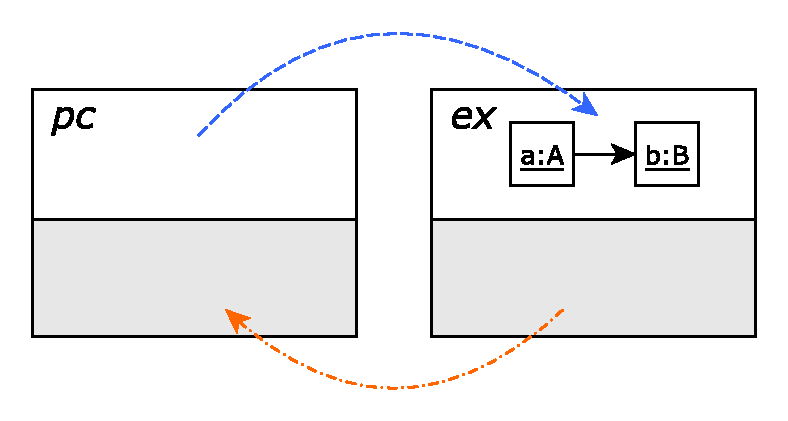
\includegraphics[width=1\textwidth]{./figures/abstraction_relation/empty_pc.pdf}
               	\caption{Abstraction holds}
               	\label{fig:empty_pc_success}
        \end{subfigure}%
        ~~\\
        \begin{subfigure}[b]{0.40\textwidth}
                \centering
                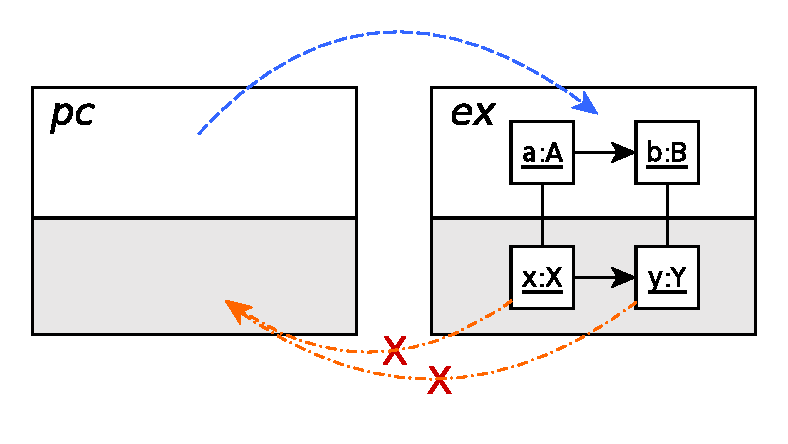
\includegraphics[width=1\textwidth]{./figures/abstraction_relation/empty_pc2.pdf}
                \caption{Abstraction does not hold}
                \label{fig:empty_pc_fail}
        \end{subfigure}%
        \caption{Abstraction of transformation executions by the empty path condition}
        \label{fig:empty_pc}
\end{figure}


The match part of the path condition represents the pre-conditions for the path condition to be true, depending on which rules have symbolically executed in the transformation. For example, if the match graph is empty, this represents all executions where no rules have executed. 

The first condition for the abstraction relation is to determine whether a typed graph injective homomorphism can be found between the match graph of the path condition, and an transformation executions. Note that in both \cref{fig:empty_pc_success} and \cref{fig:empty_pc_fail}, an empty typed graph homomorphism satisfies this condition, highlighted by blue arrows.


The second condition for the abstraction relation is whether a typed graph surjective homomorphism can be found from the transformation execution's output model to the apply graph of the path condition. This is represented by orange arrows in \cref{fig:empty_pc_success} and \cref{fig:empty_pc_fail}. This relation is surjective as there may not be any elements in the output model that are not represented by the path condition's apply graph. Note that multiple elements in the output model may match to the same element in the apply graph of the path condition. This is expected, as the structure found in the apply graph may be found multiple times in the output model.


The empty apply graph of the path condition defines no post-conditions on the output model, as no rules have executed. Note that there an empty surjective typed graph homomorphism can be found between the output model of the transformation execution in \cref{fig:empty_pc_success} and the path condition. This is intuitive, as the lack of elements in the output model means no rules have executed, which corresponds to the lack of post-conditions defined by the path condition.


In contrast, there is no surjection between the elements of the output model in \cref{fig:empty_pc_fail} and the path condition. Note that the transformation execution has elements in the output model and thus at least one rule must have executed. However, the path condition does not represent that a rule has executed. Therefore, the path condition shown does not represent this execution. 

%The fact that this transformation execution will be abstracted by at least one path condition is demonstrated by \cref{prop:pc_completeness}.



\subsubsection{Example 2 -- Non-overlapping Rule Components}


This second example shows the abstraction relation between path conditions and transformation executions, when no match element of the same type appears in multiple rule components.

For these examples, we will represent the abstraction relation with two figures. The first will demonstrate the matching performed on match and apply graphs, while the second figure focuses on traceability link matching.

Let us first examine how the injection operates between the match elements in the path condition and the transformation executions in \cref{fig:non_overlapping_match_apply} and \cref{fig:non_overlapping2_match_apply}. Note that this injection can be found in both cases.

\begin{figure}[htb]
        \centering
        \begin{subfigure}[b]{0.40\textwidth}
                \centering
                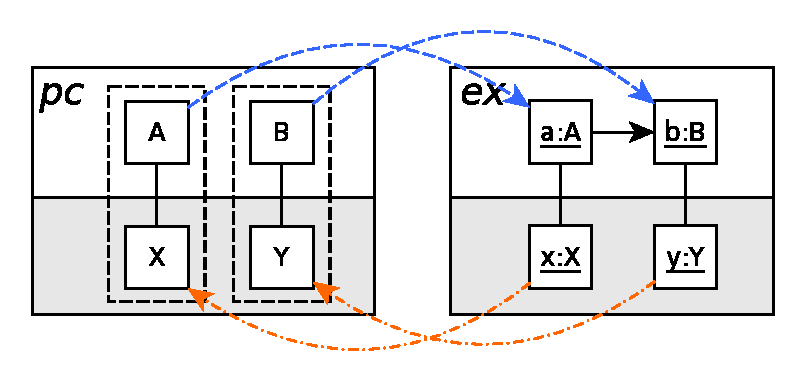
\includegraphics[width=1\textwidth]{./figures/abstraction_relation/non_overlapping.pdf}
               	\caption{Abstraction holds on match and apply graphs}
               	\label{fig:non_overlapping_match_apply}
        \end{subfigure}%
        ~~\\
        \begin{subfigure}[b]{0.40\textwidth}
                \centering
                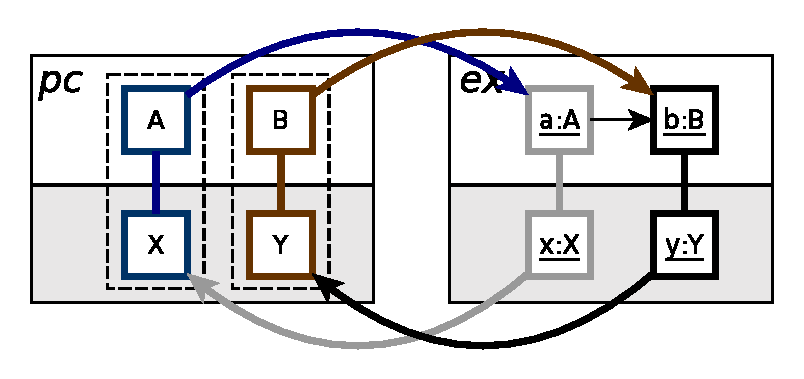
\includegraphics[width=1\textwidth]{./figures/abstraction_relation/non_overlapping_trace_links.pdf}
                \caption{Abstraction holds on traceability links}
                \label{fig:non_overlapping_trace_links}
        \end{subfigure}%
        \caption{Abstraction of transformation execution by non-overlapping rule components}
        \label{fig:non_overlapping}
\end{figure}


\begin{figure}[htb]
        \centering
        \begin{subfigure}[b]{0.40\textwidth}
                \centering
                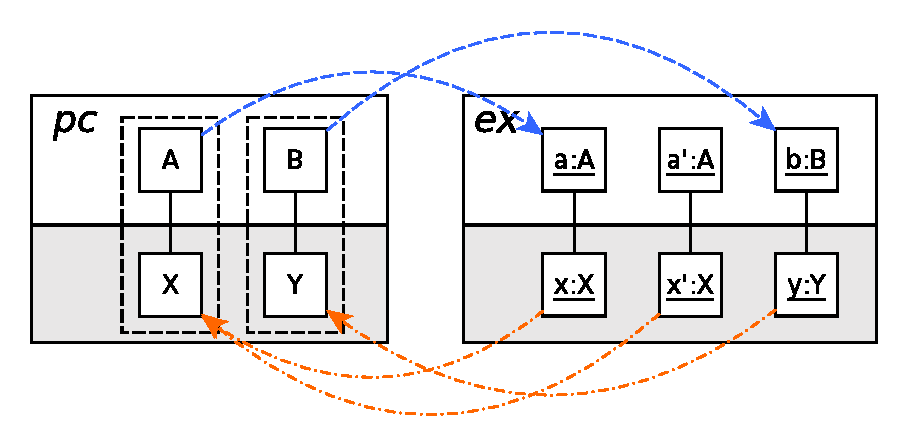
\includegraphics[width=1\textwidth]{./figures/abstraction_relation/non_overlapping2.pdf}
               	\caption{Abstraction holds on match and apply graphs}
               	\label{fig:non_overlapping2_match_apply}
        \end{subfigure}%
        ~~\\
        \begin{subfigure}[b]{0.40\textwidth}
                \centering
                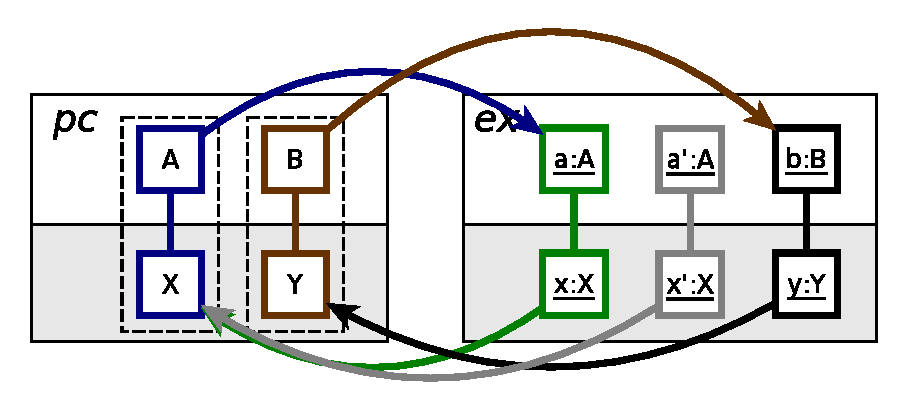
\includegraphics[width=1\textwidth]{./figures/abstraction_relation/non_overlapping2_trace_links.pdf}
                \caption{Abstraction holds on traceability links}
                \label{fig:non_overlapping2_trace_links}
        \end{subfigure}%
        \caption{Example of abstraction over multiple rule execution}
        \label{fig:non_overlapping2}
\end{figure}

Similarly, there is a surjection between the elements of the output model for both transformation execution and the apply graph of the respective path condition. Note that this surjective match also holds in \cref{fig:non_overlapping2_match_apply}, where examination of the transformation execution shows that one rule has executed twice. As mentioned before, the abstraction relation abstracts over the number of times that a rule has executed.

We also note that these matches must also match over associations between the elements, including association typing. This is not included in the figures for visual clarity.


We now examine \cref{fig:non_overlapping_trace_links} and \cref{fig:non_overlapping2_trace_links} to resolve whether the traceability links in the path condition can be found in the transformation execution. This matching is represented by the arrows from each component highlighted in a bold outline and differentiated by colour. We note that each component in the path condition can be successfully found in the transformation execution.

As well, there is a matching step from each individual traceability link in the transformation execution onto the path condition. Similar to the matching from the path condition, the bold components in the transformation execution figure are matched onto the path condition. We note that this matching is successful as well.


\subsubsection{Example 3 -- Overlapping Rule Components}
\label{subsubsec:abstraction_relation_overlapping}

For these examples, the path conditions contain overlapping rule components, i.e. separate rules share match elements of the same type. Our goal is to illustrate the interaction of rule elements, where the elements of non-dependent rules may match over the same or different elements in the transformation execution.

For example, the two rule components in \cref{fig:overlapping_match_apply} correctly match over the transformation execution shown. The abstraction relation holds due to the fact that, while match elements of the same component need to be found injectively in the execution, the injection constraint does not span multiple components. This allows the match elements from different rules to match to the same input model element.


\begin{figure}[htb]
        \centering
        \begin{subfigure}[b]{0.40\textwidth}
                \centering
                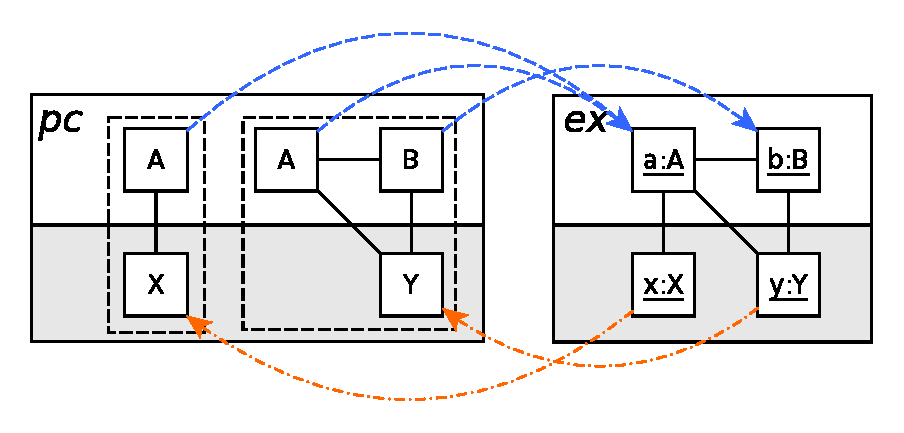
\includegraphics[width=1\textwidth]{./figures/abstraction_relation/overlapping.pdf}
               	\caption{Abstraction holds on match and apply graphs}
               	\label{fig:overlapping_match_apply}
        \end{subfigure}%
        ~~\\
        \begin{subfigure}[b]{0.40\textwidth}
                \centering
                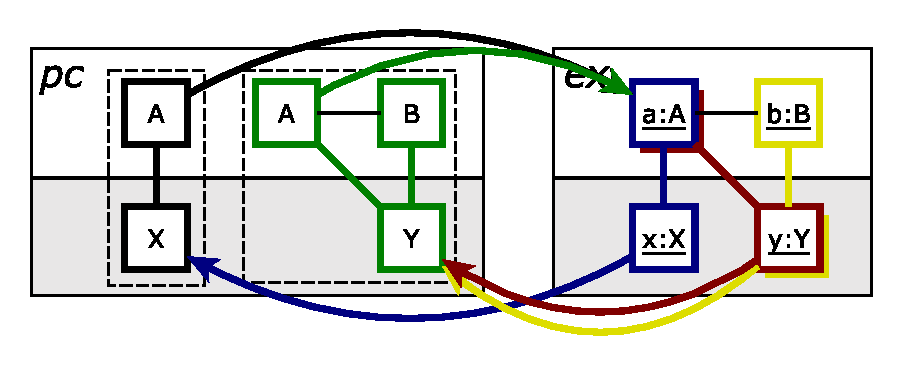
\includegraphics[width=1\textwidth]{./figures/abstraction_relation/overlapping_trace_links.pdf}
                \caption{Abstraction holds on traceability links}
                \label{fig:overlapping_trace_links}
        \end{subfigure}%
        \caption{Abstraction of transformation execution by overlapping rule components}
        \label{fig:overlapping}
\end{figure}

As well, \cref{fig:overlapping_trace_links} shows the mapping from the path condition to the transformation execution. However, note that the pattern composed of the A, B, and Y elements, along with the traceability links, is to be matched as a whole. This is to ensure that the traceability links are found in the proper configuration in the transformation execution.

We also match the traceability links from the transformation execution back onto the path condition. Again, this is to ensure that no traceability links are found in the transformation execution that have not been represented in the path condition. Three matches are performed in this step, denoted by the three arrows in the bottom of \cref{fig:overlapping_trace_links}. Each match is composed of a traceability link as well as immediately connected elements.

\begin{figure}[htb]
        \centering
        \begin{subfigure}[b]{0.40\textwidth}
                \centering
                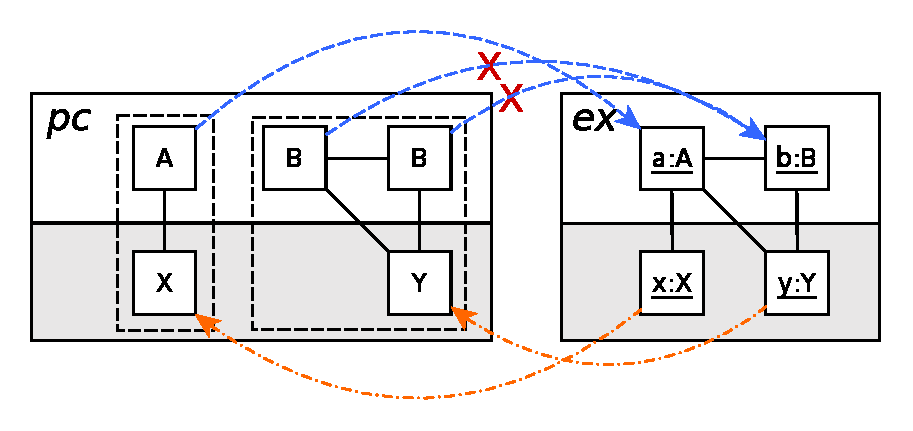
\includegraphics[width=1\textwidth]{./figures/abstraction_relation/overlapping2.pdf}
               	\caption{Elements cannot overlap within a component}
               	\label{fig:overlapping2_match_apply}
        \end{subfigure}%
        ~~\\
        \begin{subfigure}[b]{0.40\textwidth}
                \centering
                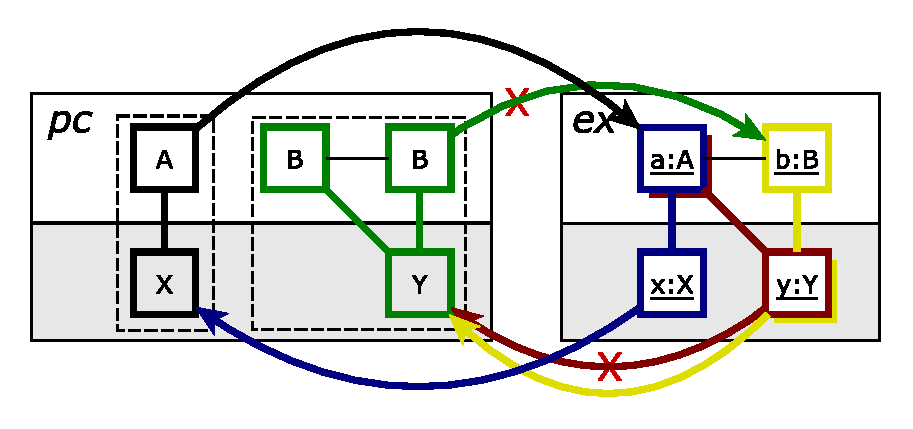
\includegraphics[width=1\textwidth]{./figures/abstraction_relation/overlapping2_trace_links.pdf}
                \caption{Traceability links cannot be found}
                \label{fig:overlapping2_trace_links}
        \end{subfigure}%
        \caption{Abstraction does not hold}
        \label{fig:overlapping2}
\end{figure}


In contrast to \cref{fig:overlapping}, \cref{fig:overlapping2} shows an example where the abstraction relation does not hold. Consider \cref{fig:overlapping2_match_apply}. Note that a component in the match graph of the path condition contains two B elements. Both of these elements must be found in the transformation execution, and thus it is not correct for them to injectively match to the same element in the input model.

As well, it is informative to examine \cref{fig:overlapping2_trace_links}. Note the one of the matches from the transformation execution attempts to match over 'a:A' and 'y:Y' elements, connected by a traceability link. Examination of the path condition shows that this traceability link is not present. Therefore, this path condition cannot accurately represent this transformation execution.


\subsubsection{Example 4 -- Indirect Links}

\begin{figure}[htb]
        \centering
        \begin{subfigure}[b]{0.40\textwidth}
                \centering
                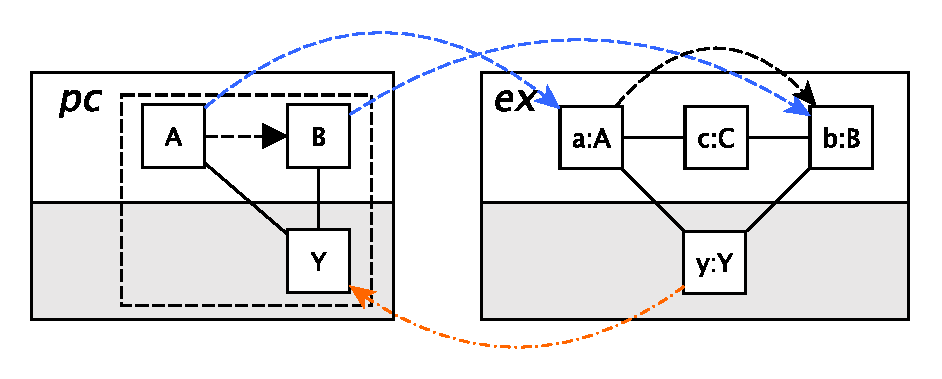
\includegraphics[width=1\textwidth]{./figures/abstraction_relation/indirect.pdf}
               	\caption{Matching over match and apply graphs}
               	\label{fig:indirect_match_apply}
        \end{subfigure}%
        ~~\\
        \begin{subfigure}[b]{0.40\textwidth}
                \centering
                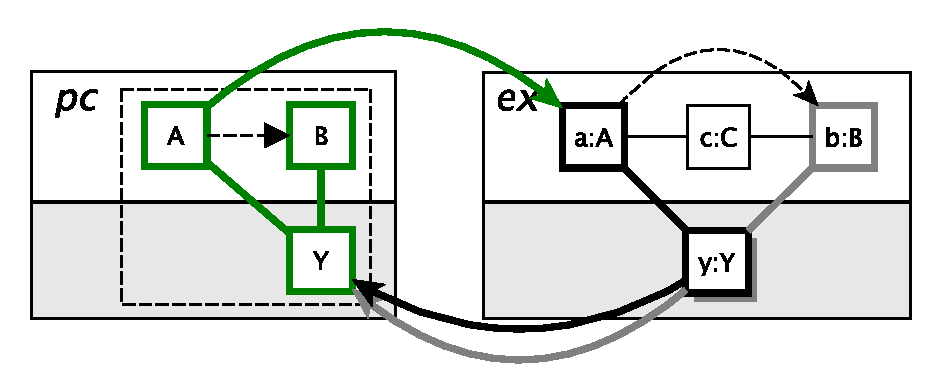
\includegraphics[width=1\textwidth]{./figures/abstraction_relation/indirect_trace_links.pdf}
                \caption{Matching over traceability links}
                \label{fig:indirect_trace_links}
        \end{subfigure}%
        \caption{Abstraction with indirect links}
        \label{fig:indirect}
\end{figure}

\begin{figure*}[htb]
        \centering
        \begin{subfigure}[b]{0.70\textwidth}
                \centering
                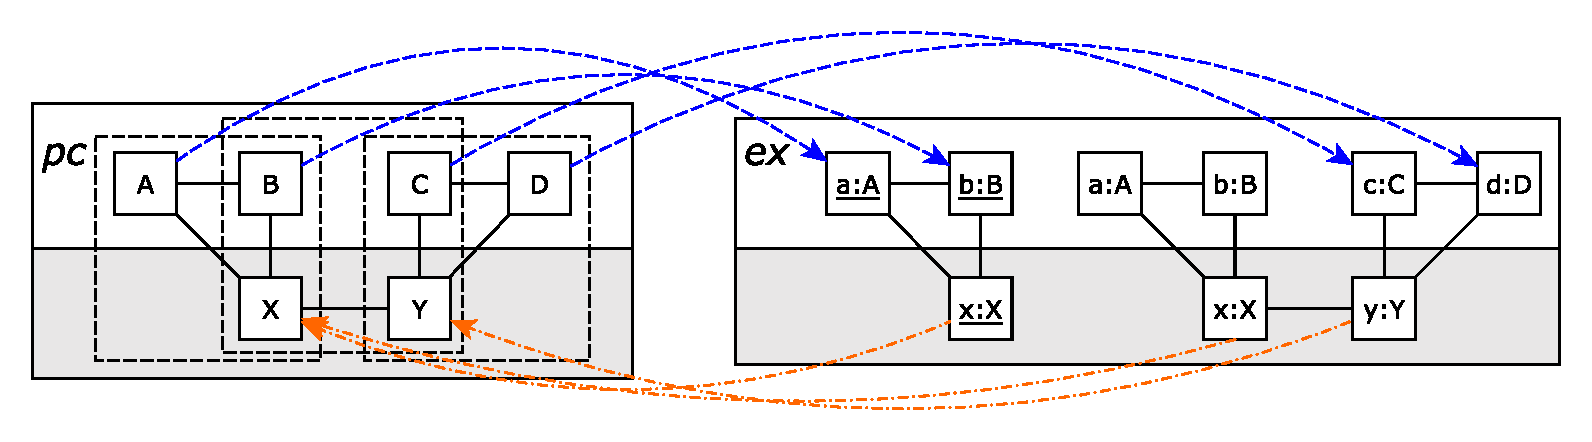
\includegraphics[width=1\textwidth]{./figures/abstraction_relation/combination.pdf}
               	\caption{Abstraction holds on match and apply graphs}
               	\label{fig:combination_match_apply}
        \end{subfigure}%
        ~~\\
        \begin{subfigure}[b]{0.70\textwidth}
                \centering
                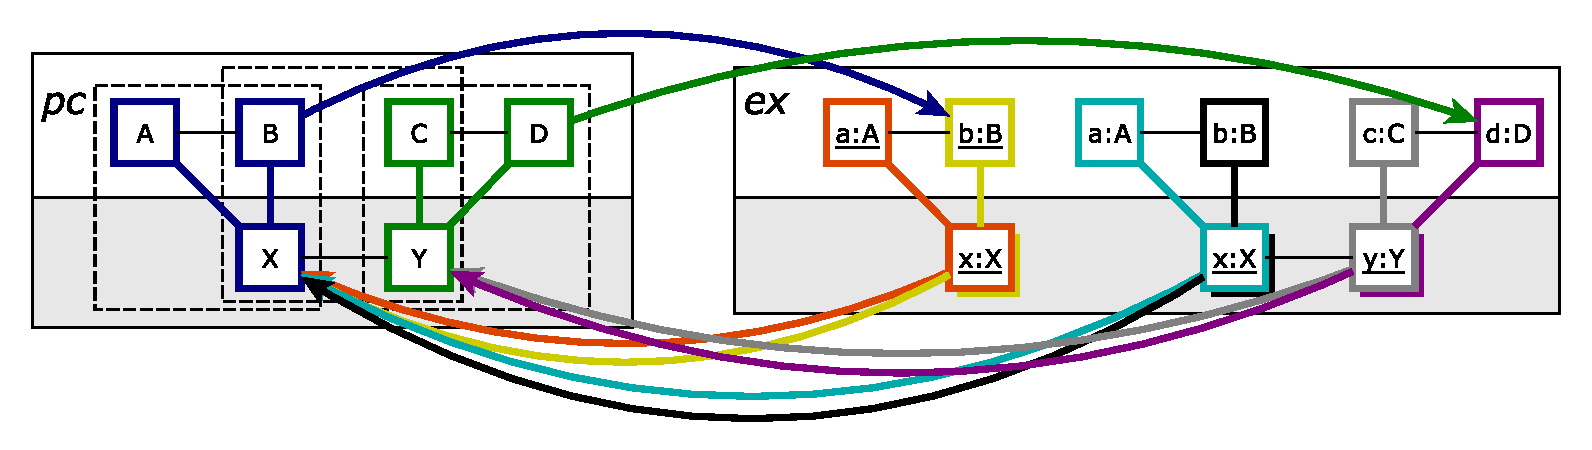
\includegraphics[width=1\textwidth]{./figures/abstraction_relation/combination_trace_links.pdf}
                \caption{Abstraction holds on traceability links}
                \label{fig:combination_trace_links}
        \end{subfigure}%
        \caption{Abstraction where path condition has combined rules}
        \label{fig:combination}
\end{figure*}

We now present a path condition  in \cref{fig:indirect_match_apply} that includes indirect links. In this case, for the injective match to hold, the elements at both ends of the link must be found, and there must be an indirect link between the matched elements and between the elements in the transformation execution.

Note that the indirect link between elements $a:A$ and $b:B$ in the transformation execution is added by the containment transitive closure $Input^{*}$ in proposition~\ref{eq:abstr_input_output} of \cref{def:abstraction_pc_ex} to allow matching indirect links. Note also that, for the sake of our example, we are assuming that the links between $a:A$, $b:b$ and $c:C$ are containment relations.

\cref{fig:indirect_trace_links} highlights the structures involved in matching over traceability links. From the path condition, the structure contains the A, B, and Y elements with connected traceability links. From the transformation execution, there are two structures to be found in the path condition denoted in bold in the transformation execution. The matching of all structures can be successfully performed, and thus this abstraction relation holds.


%Note that only the match graph of the path condition may include an indirect link.



\subsubsection{Example 5 -- Combined Rules}



\cref{fig:combination} shows a path condition that is composed of a multitude of rules which have been combined in the path condition generation algorithm. Each individual rule is surrounded by dashed lines.

Note that the matching on the match and apply graphs in \cref{fig:combination_match_apply} is similar to other examples. The combined rules can be considered as a single graph for the abstraction relation.

\cref{fig:combination_trace_links} shows the matching when multiple traceability links are present in the transformation execution. Note that each individual traceability link and the connected elements are matched onto the path condition.

\subsection{Validity and Completeness}
\label{subsec:abstraction_relation_validity_completeness}

In this section, we discuss the validity and completeness of the abstraction relation. Only proof sketches are presented here for \cref{prop:pc_validity} and \cref{lem:uniqueness}, while more complete proofs are found in \cref{sec:val_complete_path_cond_gen}, in the proofs of \cref{prop:pc_validity_appendix} and \cref{lem:uniqueness_appendix} respectively.


%\newpage
\begin{proposition}{(Validity)}
\label{prop:pc_validity}
Every path condition abstracts at least one transformation execution.
\end{proposition}
\begin{ps}

Let $tr\in \textsc{Transf}^{sr}_{tg}$ be a DSLTans transformation. We wish to demonstrate that, for all path conditions $pc\in \textsc{Pathcond}(tr)$, there exists a transformation execution $ex\in \textsc{Exec}(tr)$ of the set of
rules used to build $pc$ such that $pc$ abstracts $ex$, as formally expressed in \cref{def:abstraction_pc_ex}. We can prove this property by induction on the set of transformations $\textsc{Transf}^{sr}_{tg}$ (see \cref{def:layer_transformation}), as follows:

\begin{itemize}
  \item \emph{Base case:} the base case is when $tr$ is the empty
  transformation. In this case, according to \cref{def:path_cond_gen} only the
  empty path condition $\epsilon_{pc}$ exists in the path condition set. We thus
  need to demonstrate that the empty path condition abstracts the empty
  transformation execution $\epsilon_{ex}$, as well as any execution for which
  the input model is never matched by any rule (consequently having an empty
  output model). For any of these transformation executions, Proposition~\ref{eq:abstr_input_output} of the abstraction relation definition is satisfied, as no rule copy exists in the path condition and the output of the transformation execution is empty -- empty typed graph homomorphisms thus satisfy the all the conditions of the proposition. Proposition~\ref{eq:abstr_trace} of the abstraction relation definition also trivially holds because no traceability links exist either in the path condition or in any of the considered executions.
  
%   This is so because:
%   1) the empty typed graph homomorphism is an injective typed graph homomorphism
%   between the match part of the empty path condition and any input model; and 2) as
%   well as a surjective typed graph homomorphism between an empty output model
%   and the apply part of the empty path condition.
 
\item \emph{Inductive case:} assuming every path condition generated for a transformation $tr$ abstracts at least one transformation execution, we need to show that every path condition generated for a transformation $tr'$, resulting from adding a layer $l\in \textsc{Layer}^{sr}_{tg}$ to $tr$, will also abstract at least one transformation execution. 
\end{itemize}

In order to demonstrate the inductive case we need to show the property holds for all path conditions resulting from combining the rules of layer $l$ with any path condition generated for $tr$. These path conditions for transformation $tr'$ are built as expressed in \cref{def:path_cond_layer_comb}. According to this definition, path conditions for $tr'$ are built by incrementally combining the path conditions generated for $tr$ with a rule of layer $l$, until all the rules in $l$ have been treated. We can thus again use induction for this proof, this time on the set of possible layers $\textsc{Layer}^{sr}_{tg}$. 

\begin{itemize}
  \item \emph{Base case:} this is the case where layer $l$ contains no rules. In this case, by the base case of \cref{def:path_cond_layer_comb}, no new path condition is added to the set of path conditions generated for the transformation $tr$. As such the $tr=tr'$ and by induction hypothesis the property trivially holds for all path conditions generated for $tr'$.
  
  \item \emph{Inductive case:} for the inductive case (transitive case of \cref{def:path_cond_layer_comb}) we need to show that, assuming the property holds for all path conditions generated for a transformation $tr$, then the property will also hold for a transformation $tr'$ -- where $tr'$ results from adding a new rule $rl$ to the last layer of $tr$. We will thus need to consider the four cases of rule combination:\vspace{.2cm} 
 
\begin{enumerate}
\item\label{lab:rule_case1} Rule $rl$ has no dependencies (\cref{def:rule_comb_no_dependencies}).
\item\label{lab:rule_case2} Rule $rl$ has dependencies and cannot execute (\cref{def:rule_comb_unsatisfied}).
\item\label{lab:rule_case3} Rule $rl$ has dependencies and may and/or will execute (\cref{def:rul_comb_partial_total}).
\end{enumerate}

The property trivially holds for case~\ref{lab:rule_case2}, given that no new path conditions are added to the path condition set generated for $tr$ and that the property holds for $tr$ by induction hypothesis. When a rule $rl$ is added to the last layer of $tr$ such that cases~\ref{lab:rule_case1} or~\ref{lab:rule_case3} occur, then the property can be shown to hold for $tr'$ as follows: 1) choose for a general path condition $pc$ generated for $tr$ an execution $ex$ such that $pc$ abstracts $ex$; 2) build an input model $m$ as the result of uniting the input model of $ex$ with a model that can be matched by $rl$; 3) execute $tr'$ having as input model $m$ to produce transformation execution $ex'$; and finally 4) demonstrate $ex'$ is abstracted by the path condition $pc'$ resulting from combining $pc$ with $rl$ whether rule $rl$ does not depend on $pc$ or rule $rl$ depends on $pc$ and may and/or will execute.
\end{itemize}
\end{ps} 


\begin{proposition}{(Completeness)}
\label{prop:pc_completeness}
Every transformation execution is abstracted by one path condition.
\end{proposition}
\CatchFileBetweenTags{\pathgencompletenessproof}{text/definitions}{pathgencompletenessproof}{\pathgencompletenessproof} 

% Our path conditions construction algorithm takes all possible interactions of rules
% into account:
% \begin{enumerate}
% \item When building the path conditions for one layer we have built all
% the combinations of rules, as well as their possible interactions through
% \emph{disambiguation};
% \item When combining the path conditions from different layer different layers
% we have considered the cases where no interactions exist, or where backward
% links in rules requires certain certain elements to already exist in the
% generated model thus far.
% \end{enumerate}
% Note that, given the considered subset of DSLTrans constructs as described
% in \cref{sec:dsltrans}, no additional cases of rule interaction other than the
% ones described above need to be considered.
% From \cref{prop:pc_validity} we also know that at least one concrete
% transformation execution exists per path condition. In the proof of
% \cref{prop:pc_validity} we have built, for each path condition $A$,
% the simplest transformation execution that is abstracted by $A$. These
% transformation executions produce one instance of each element and association
% present in the apply pattern of $A$. However, given
% \cref{def:instance_pc_ex} in \cref{sec:proofs} (abstraction of
% a transformation execution by a path condition), an infinite amount of
% transformation executions are always abstracted by $A$. These executions
% correspond to the generation of output models holding an arbitrarily large
% amount of the elements and associations while still being abstracted by $A$.
% Because we have considered all possibilities of execution in our path condition
% construction algorithm, the union of all transformation executions built for
% each path condition constitutes the complete, infinite set of transformation
% executions. We thus know that every possible transformation execution is
% abstracted by at least one path condition.


% Note that we do not provide any guarantee that the same transformation execution
% cannot be abstracted by two different path conditions. Although given our symbolic
% execution assumptions we believe this to be the case, further mathematical
% exploration of this issue is necessary. Given however the fact that our
% verification algorithm exhaustively explores all path conditions, it is
% sufficient for the property proof to provide a \emph{no} result in the analysis
% of a path condition for the result of the verification of the property to be
% \emph{no}. \levi{keep this?}

\begin{lemma} (Uniqueness) 
\label{lem:uniqueness}
A transformation execution is abstracted by exactly one path condition.
\end{lemma}
\begin{ps}
Let $tr\in \textsc{Transf}^{sr}_{tr}$ be a model transformation. We will demonstrate that two different path conditions\\$pc_1, pc_2\in \textsc{Pathcond}(tr)$ cannot exist such that we have a transformation execution $ex\in \textsc{Exec}(tr)$ where $ex\Vvdash pc_1$ and $ex\Vvdash pc_2$.

We will do so by attempting to to build an $ex\in \textsc{Exec}(tr)$ such that $ex\Vvdash pc_1$ and $ex\Vvdash pc_2$ and demonstrating that it is always the case that such is not possible. In order to structure our argumentation, we will consider two cases:
% \levi{the contradiction happens because at each point of the execution, when a rule is added any two path conditions from the existing set of path conditions will represent different executions. At all points if we consider two path conditions in the PC set we have that two different executions can be created if we find a model that satisfies the first condition of the abstraction relation, and it is always the case that none of those two executions can be abstracted by the two path conditions simultaneously.}
\begin{enumerate}
  \item\label{item:uniqueness_rule_no_dep} the case where no rules in $tr$ have dependencies.
  \item\label{item:uniqueness_rule_has_dep} the case where some rules in $tr$ have dependencies.
\end{enumerate}

We start by considering that $tr$ falls into case~\ref{item:uniqueness_rule_no_dep} above. By~\cref{def:path_cond_gen} of path condition generation, each rule appears at most once in a path condition. Also, by construction, each path condition always contains a different combination of rules. We additionally know from \cref{def:layer_transformation} that the rules that compose $tr$ necessarily have non-overlapping matchers. We can nonetheless build a model $m$ as the typed graph union of two input models $m_1$ and $m_2$, where injective typed graph morphisms can be found between the match parts of the rule copies that form $pc_1$, and $m_1$. Injective typed graph morphisms can be found as well between the match parts of the rules that form $pc_2$, and $m_2$. We thus know that injective typed graph morphisms can be found between the rule copies that compose $pc_1$ and $pc_2$, and $m$. This satisfies the first condition of \cref{eq:abstr_input_output} in ~\cref{def:abstraction_pc_ex} of abstraction relation. 

Let us now consider that $ex_1$ and $ex_2$ are obtained by executing the transformations rules combined into $pc_1$ and $pc_2$, having $m$ as input model. As mentioned above, we know that the rules in $pc_1$ and $pc_2$ are not completely overlapping. This means that, due to the way in which $m$ is built (explained above), $m$ will always have at least one input that is matched by rules of $pc_1$ but not by rules of $pc_2$ (and vice-versa). Thus, when the transformation rules combined into $pc_1$ execute having $m$ as an input model, there will always exist a traceability link generated between an input and an output element of $m$ that is not generated when the transformation rules combined into $pc_2$ execute having $m$ as an input model (and vice-versa). As such, we have that $ex_1$ is always different from $ex_2$ by at least one traceability link. Given that this traceability link is symbolically represented in either $pc_1$ or $pc_2$ (but not in both), according to condition \cref{eq:abstr_trace} in \cref{def:abstraction_pc_ex} it cannot be that either $pc_1$ or $pc_2$ abstract $ex_1$ and $ex_2$ simultaneously.\\\\
We will now analyse the scenario where $tr$ falls into case~\ref{item:uniqueness_rule_has_dep} above, where some rules in $tr$ have dependencies. For this case, assume we have a path condition $pc_1$ contained in the set of path conditions generated for $tr$, considering layers up to layer $l$ of $tr$ have executed. Assume also we have a rule $rl$ of layer $l+1$ of $tr$ that has dependencies and can be combined with $pc$. If rule $rl$ is totally combined with path condition $pc_1$, according to \cref{def:rul_comb_partial_total} and \cref{fig:multiple_total_satisfied_dependencies}, then nothing needs to be shown as $pc_1$ is not kept in the path condition set but rather replaced by its combination with $rl$. However, in case rule $rl$ is partially combined with $pc$, as defined in \cref{def:rul_comb_partial_total} and \cref{def:comb_path_cond_rule_single}, then multiple path conditions are generated and additionally $pc_1$ is kept in the path condition set.\\The proof will be complete once it is shown that for the path conditions that are generated when rules are partially combined, it is also the case that no two path conditions can abstract the same execution. This last part of the proof can be built in an analog fashion to the construction of the proof for point~\ref{item:uniqueness_rule_no_dep}. As previously mentioned, the complete proof can be found as \cref{lem:uniqueness_appendix} in \cref{sec:val_complete_path_cond_gen}.

\end{ps}



\section{Building Path Conditions}
\label{sec:building_pcs}

This section will present how path conditions are structured to represent symbolic rule execution. As well, we present our approach to building a set of path conditions to represent all executions of a DSLTrans transformation.

\subsection{Symbolic Execution}

Our algorithm operates on the principle of symbolic execution to build up these
path conditions. In order to explain the concept of symbolic execution of a
transformation, let us make an analogy with program symbolic execution as
introduced by King in his seminal work ``\emph{Symbolic Execution and Program
Testing}''~\cite{DBLP:journals/cacm/King76}. According to King, a symbolic
execution of a program is a set of \emph{constraints} on that program's
\emph{input variables} called \emph{path conditions}. Each \emph{path condition}
describes a traversal of the conditional branching commands of that program. A
\emph{path condition} is symbolic in the sense it \emph{abstracts} as many
concrete executions as there are instantiations of the path condition's
variables that render the path condition's constraints true.

We can transpose this notion of symbolic execution to model transformations. The
analog of an input variable in the model transformation context are
\emph{metamodel classes, relations and attributes}. As program statements impose
constraints on input and output variables during symbolic execution,
transformation rules impose conditions on which metamodel elements are
instantiated during a concrete transformation execution, and how that
instantiation happens. As well, rules in a model transformation are implicitly
or explicitly scheduled. These control and/or data dependencies must be
taken into consideration during path condition construction.

As in program symbolic execution, each path condition in our approach \emph{abstracts} as many concrete executions as there are input/output models
that satisfy them. This is formulated as an \emph{abstraction relation} as further explained in \cref{sec:abstraction_relation}.

In what follows we will examine in more detail how these symbolic execution
principles can apply to the verification of model transformations.


\subsection{Path Conditions}
\label{sec:gen_path_conds}

In order to present the intuition of path conditions and symbolic executions, we
first discuss the idea of \textit{rule combinations}.

As seen in \cref{sec:dsltrans}, a layer in a DSLTrans transformation contains a
number of rules.  We can create a set of rule combinations for this layer by
taking the powerset of all rules in that layer. Each rule combination in this
set will represent all possible transformation executions where the rules in
that combination would execute.

For example, in \cref{fig:rule_combos2}, the rule combination marked `AC'
represents the set of transformation executions where the rules A and C would
execute and no others. Another rule combination marked `A' represents the
transformation executions where only rule A would execute.

\begin{figure}[h!] \centering 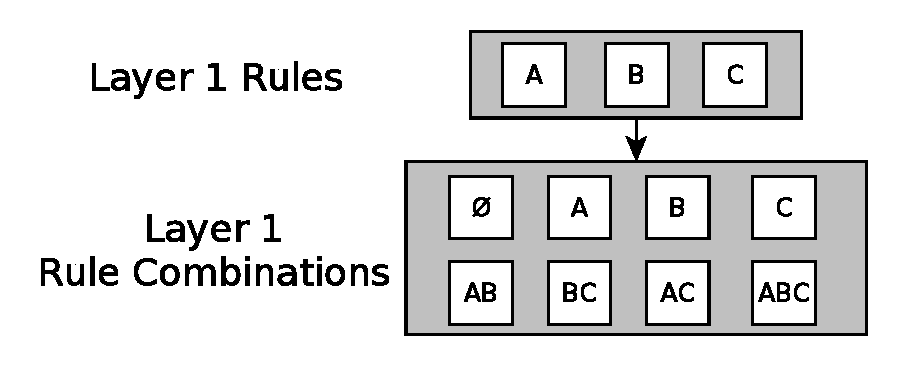
\includegraphics[width=.40\textwidth]{./figures/overview/rule_combos.pdf}
	\caption{Rule combinations created for a transformation layer}
	\label{fig:rule_combos2}
\end{figure}

Note that within these rule combinations, the number of times a rule has
executed is abstracted. Either a rule has executed zero times, and the rule is
not represented in a rule combination, or the rule has executed some finite
number of times and it is represented. This abstraction is key to our approach,
as it allows us to create a finite set of path conditions to abstract over an
infinite set of transformation executions, as seen in
\cref{sec:abstraction_relation}.

We also note that rule \textit{combinations} are created, and not rule
\textit{permutations}. This follows from the semantics of \\DSLTrans as described
in \cref{sec:dsltrans}, as transformation rules in a layer will execute in a
non-deterministic order but produce a deterministic result, by construction of the semantics of DSLTrans. As a final
note, the transformation executions that these rule combinations represent always terminate, also by construction of the semantics of DSLTrans~\cite{DBLP:conf/sle/BarrocaLAFS10}.

We base our concept of path conditions on these rule combinations. However, as
DSLTrans allows for dependencies between rules, we cannot create path conditions
for the transformation by taking the powerset of all rules. Instead, our
approach must move layer-by-layer and resolve the dependencies between rules.
The next two sections will introduce the concepts of traceability and dependency, before we
briefly discuss the syntax and semantics of path conditions themselves.

\subsubsection{Traceability}
\label{subsubsec:traceability}

DSLTrans rules allow for dependencies to be specified on which elements of the
output model were created from specific elements of the input model. To resolve
these dependencies, traceability information for the transformation is created
during the execution of a DSLTrans model transformation~\cite{DBLP:conf/sle/BarrocaLAFS10}.
In our verification approach, we store this same information as symbolic \emph{traceability links}, in
order to record which elements belong to the same DSLTrans rule.


At a particular point in the path condition construction process, symbolic traceability links are built for
each rule as follows: for all match and apply elements of a rule, given a match
element belonging to the match graph of a rule and an apply element belonging to
the apply graph of the same rule, a symbolic traceability link is built between the two
if the apply element is not connected to a backward link (as explained below).
This is intuitive: traceability links are built between a newly generated
element in the output model, and the elements of the input model that originated
it.

\begin{figure}[htb]
        \centering
        \begin{subfigure}[b]{0.24\textwidth}
                \centering
                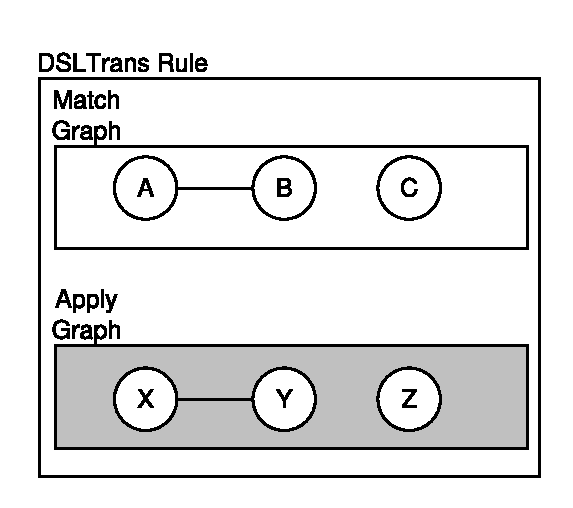
\includegraphics[width=1\textwidth]{./figures/building_path_conditions/traceability_links.pdf}
                \caption{Before symbolic traceability links added}
                \label{fig:traceability_links1}
        \end{subfigure}%
        ~~
        \begin{subfigure}[b]{0.235\textwidth}
                \centering
                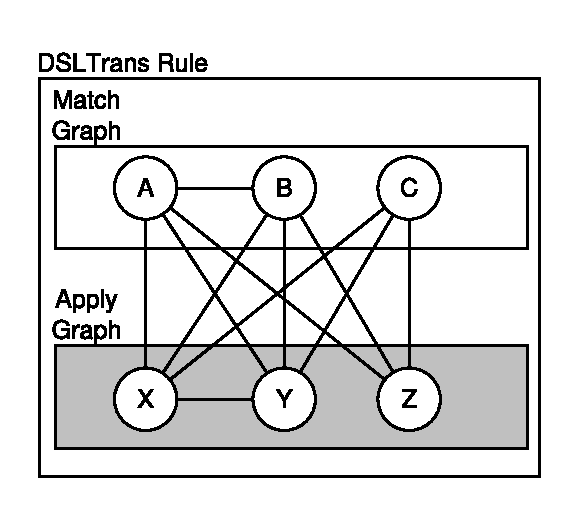
\includegraphics[width=1\textwidth]{./figures/building_path_conditions/traceability_links2.pdf}
                \caption{After symbolic traceability links added}
                \label{fig:traceability_links2}
        \end{subfigure}%
        \caption{Symbolic traceability links created for an abstract DSLTrans rule}
        \label{fig:trace_links}
\end{figure}

An example of the symbolic traceability link creation process is shown in
\cref{fig:trace_links}. Note that symbolic traceability links are a solid line between
match and apply elements in our visual notation.



\subsubsection{Backward Links}
\label{subsubsec:backward_links}

The dependencies in a DSLTrans rule are specified using the \textit{backward link} construct, as further detailed in \cref{subsec:DSLTrans_constructs} and \cref{def:transformation_rule}. \cref{subsubsec:resolve_dependencies} will discuss how these dependencies are then resolved during our symbolic execution approach.

\cref{fig:backward_links} demonstrates how backward links are used \\within a rule. The rule shown contains a backward link, which defines the dependency that an element of type X was created from an element of type A, and an element of type Y was created from an element of type B. If this dependency is satisfied, then another element of type Z should be created. This element should be associated with the Y element.

\begin{figure}[htb]
        \centering
        \begin{subfigure}[b]{0.235\textwidth}
                \centering
                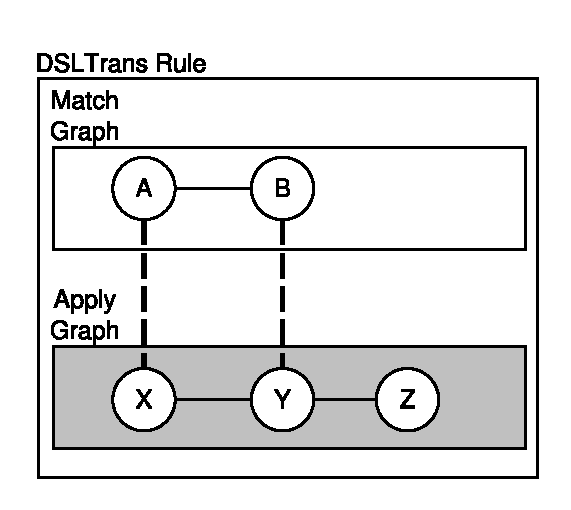
\includegraphics[width=1\textwidth]{./figures/building_path_conditions/backward_link.pdf}
                \caption{Rule with backward links (dashed lines)}
                \label{fig:backward_links}
        \end{subfigure}%
        ~~
        \begin{subfigure}[b]{0.235\textwidth}
                \centering
                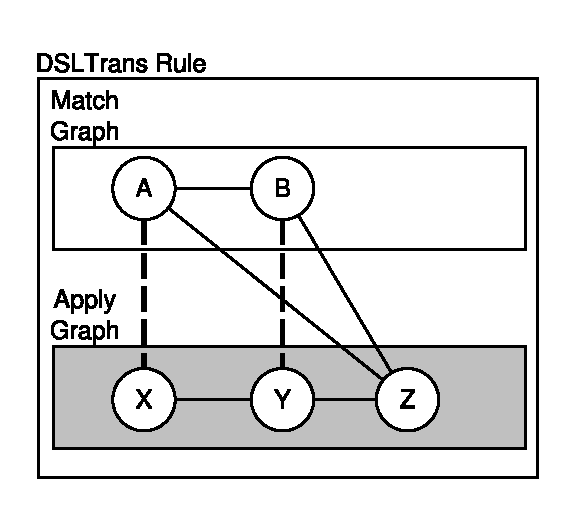
\includegraphics[width=1\textwidth]{./figures/building_path_conditions/backward_link2.pdf}
                \caption{Traceability links added\\~}
                \label{fig:backward_links2}
        \end{subfigure}%
        \caption{Adding traceability links to an abstract DSLTrans rule with backward links}
        \label{fig:back_links}
\end{figure}

\cref{fig:backward_links2} shows the rule after symbolic traceability links have been added. Two symbolic traceability links are created from the Z element to the A and B elements in the match graph to store traceability information. Note that no symbolic traceability links are built between two elements connected by backward links, as these links have already been built in a previous layer.



% \begin{definition}{Rule Traceability}
% 
% Let $rl = \big\langle V,E,st,\tau \big\rangle$ be a transformation
% rule. $trace_{\langle
% V_{\Delta},E_{\Delta},st_{\Delta},\tau_{\Delta}\rangle}(\langle
% V,E,st,\tau\rangle) = \langle V,E',st',\tau'\rangle$ where we have that
% $E\subseteq E'$, $st\subseteq st'$, $\tau \subseteq \tau'$ and if
% $v_1\xrightarrow{e} v_2\in E'\setminus E$ then $v_1\in Output(V_{\Delta})$,
% $v_2\in Input(V)$ and $\tau'(e)=trace$.
% \end{definition}


\subsubsection{Syntax and Semantics}
\label{subsubsec:path_condition_creation}

A path condition represents the symbolic execution of a set of DSLTrans rules, similar to a rule combination as explained above. Again, we use an abstraction over the number of times a rule has symbolically executed. Each path condition will represent that a rule has not executed, or has executed one or more times.

The path condition generation algorithm will symbolically combine transformation rules into a path condition. Each path condition will then abstract a set of concrete transformation executions, as defined by our abstraction relation in \cref{sec:abstraction_relation}.

As seen in the rest of this section, the structure of path conditions is similar to that of DSLTrans rules. The match graph of a path condition represents a pattern that must be present in the input model of the transformation, while the apply graph is a pattern which will be instantiated in the output model of the transformation. Symbolic traceability links are also kept between elements in the match and apply graphs to retain traceability information.

The formal definition of a path condition is presented in \cref{def:path_condition}.

\begin{definition}{Path Condition\\}
\label{def:path_condition}
\CatchFileBetweenTags{\pcdef}{text/definitions}{pcdef}{\pcdef}
\end{definition}

\CatchFileBetweenTags{\pc}{text/definitions}{pc}{\pc}

\subsection{Path Condition Generation Algorithm}
\label{sec:gen_all_pcs}

 This section will describe how path conditions are constructed for a DSLTrans transformation using our approach.

\cref{fig:next_layer} outlines the path condition generation algorithm. The algorithm will examine each transformation layer in turn. Path conditions from the previous layer will be combined with rules from the current layer to create a new set of path conditions. This new set of path conditions will then be combined with the rules from the next layer to produce yet another set of path conditions, and so on. At the end of the algorithm, a complete set of path conditions for the entire transformation will have been produced. 

\begin{figure*}[htb]
        \centering
        \begin{subfigure}[b]{0.34\textwidth}
                \centering
                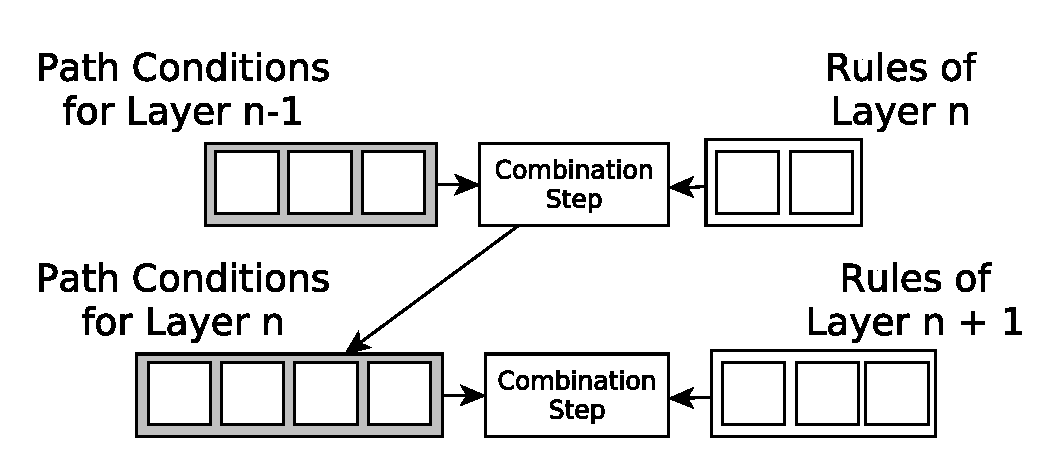
\includegraphics[width=1\textwidth]{./figures/building_path_conditions/next_layer.pdf}
                \caption{Previous path conditions are combined\\ with rules}
                \label{fig:next_layer}
        \end{subfigure}%
        ~~
        \begin{subfigure}[b]{0.34\textwidth}
                \centering
                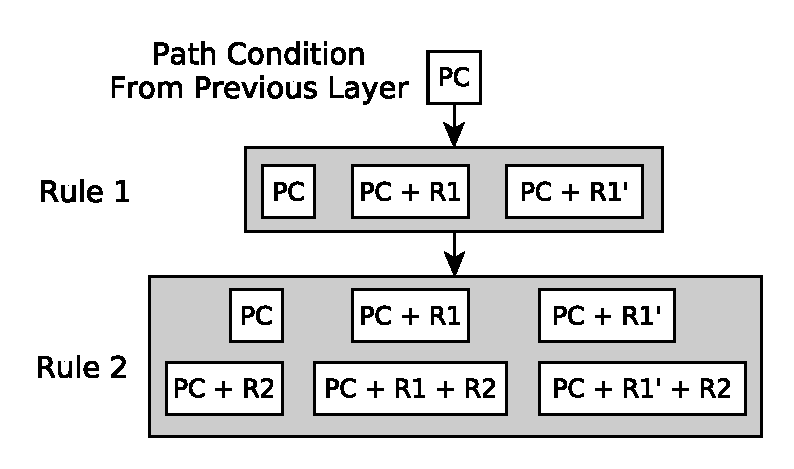
\includegraphics[width=1\textwidth]{./figures/overview/layers_pc.pdf}
                \caption{Combining a path condition with two rules\\~}
                \label{fig:layers_pc2}
        \end{subfigure}%
        
       
         \caption{Two components in the path condition creation process}
         \label{fig:combining_path_conditions}
\end{figure*}

We now define what is occurring in the `combination step' in \cref{fig:next_layer}. This step begins by selecting each path condition in the working set, one at a time. Note that at the beginning of the path condition creation process, this working set consists of an empty path condition.

A new set of path conditions will then be created by sequentially combining each rule in the layer with the path condition selected. Recall that a path condition represents a set of rules that have symbolically executed, thereby abstracting a set of transformation executions through our abstraction relation. Combining a path condition with a rule will produce one or more path conditions depending on how the rule combines with the rules already represented by the path condition. The pre- and post- conditions defined by the path condition will be modified according to the elements found in that rule. 

Each of the new path conditions created from combining a rule with a path condition will then be combined with the next rule in the layer. A small example is shown in \cref{fig:layers_pc2}, where a path condition is combined with two rules. Note that a rule can combine with a path condition in multiple ways (differentiated by prime marks in the figure). \Cref{fig:all_pcs2} shows how path conditions from the previous layer are sequentially combined with all the rules from the current layer. All the path conditions for the layer are then collected to produce the final working set of path conditions for the layer.

        \begin{figure}[bht]
                 \centering
                  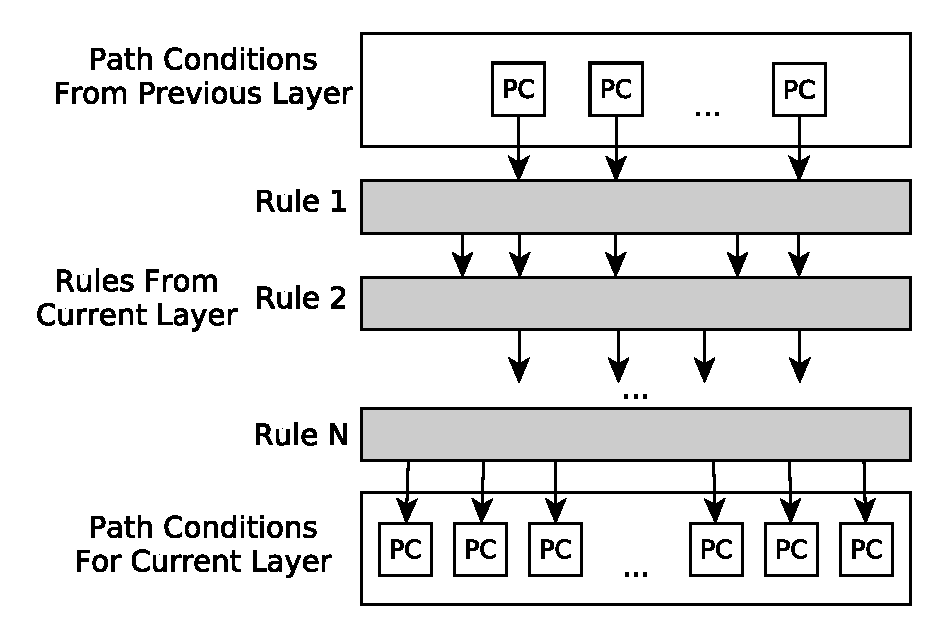
\includegraphics[width=.38\textwidth]{./figures/overview/all_pcs.pdf}
                 \caption{Creating all path conditions for a layer}
                 \label{fig:all_pcs2}
         \end{figure}
         
\subsection{Combining a Path Condition with a Rule}
We will now examine the combination step between one path condition and one rule, which produces a set of new path conditions. A formal and generic definition of this step will be presented first, before we explain the specialized combination possibilities with figures and informal text.

\begin{definition}{Combination of a Path Condition with a Rule}
\label{def:combine_pc_with_rule}

\CatchFileBetweenTags{\pccfrc}{text/definitions}{pccfrc}{\pccfrc}
\end{definition}

\CatchFileBetweenTags{\pccfrctext}{text/definitions}{pccfrctext}{\pccfrctext}

We will now discuss the combination step possibilities. Let PC be the path condition selected from layer n-1, and R the rule selected from layer n. When PC and R are combined, there are four possibilities based on the dependencies between PC and R:

\begin{enumerate}
\item R has \textbf{no} dependencies
\item R has dependencies and \textbf{cannot} execute
\item R has dependencies and \textbf{may} execute
\item R has dependencies and \textbf{will} execute
\end{enumerate}

These dependencies are defined by the backward links within R. As mentioned in \cref{subsubsec:traceability}, backward links enforce that the elements in the apply graph were created by the connected elements in the match graph. In the context of combining a rule and a path condition, these backward links define dependencies between the rule and the elements created by the rules represented by the path condition. 

The below figures will demonstrate the four cases above. As a reminder of visual notation, the backward links are dashed lines between the match and apply graphs of the rule and path condition, while symbolic traceability links are solid lines between the two graphs.

\subsubsection{No Dependencies}
\label{enum:no_back}

The rule R has a match graph which represents its pre-conditions. For a particular transformation execution, it is possible that this match graph would not match a specific input model, and thus R would not execute in these transformation executions. To represent all such transformation executions where the rule R would not execute, PC is copied unchanged to the new set of path conditions.

To represent the transformation executions where the match graph of R would match, and therefore R would execute, a new path condition is produced which consists of the union between R and PC. This situation is
seen in \cref{fig:no_dependencies} and formally defined in \cref{def:rule_comb_no_dependencies}.

\begin{figure}[bt] \centering 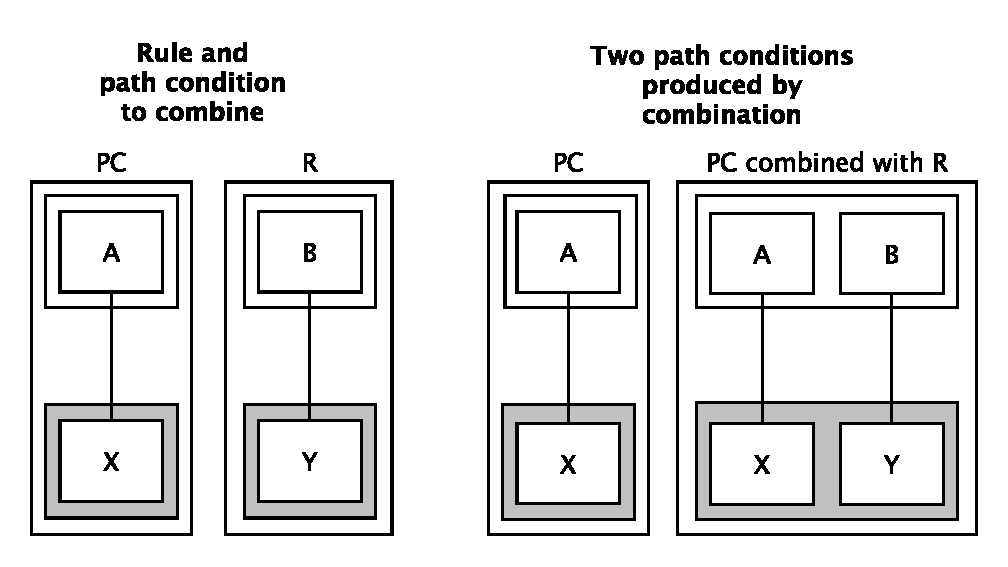
\includegraphics[width=0.44\textwidth]{./figures/building_path_conditions/no_dependencies.pdf}
	\caption{R has no dependencies}
	\label{fig:no_dependencies}
\end{figure}

% \begin{definition}{No Dependencies Between a Rule and a Path Condition}
% 
% \levi{FIX}
% Let $A=\langle V,E,st,\tau\rangle, B=\langle V',E',st',\tau'\rangle\in \textsc{Pathcond}^{sr}_{tg}$ be two path conditions. We say that $R$ does not depend on $PC$ if and only if $\nexists e\in E'\,.\,\tau'(e)=backward$.
% \end{definition}

\begin{definition}{Path Condition and Rule Combination -- No Dependencies\\}
\label{def:rule_comb_no_dependencies}
\CatchFileBetweenTags{\nodeps}{text/definitions}{nodeps}{\nodeps}

\end{definition}

\CatchFileBetweenTags{\nodepstext}{text/definitions}{nodepstext}{\nodepstext}

\subsubsection{Resolving Dependencies}
\label{subsubsec:resolve_dependencies}
If R contains backward links and thus R defines dependencies on PC, then we need to analyse whether PC can satisfy those dependencies. This is done by matching the backward links in R over the symbolic traceability links in PC. Note that symbolic traceability links in R are not required to be found in PC, and that only backward links define dependencies.

\paragraph{Unsatisfied Dependencies}


If the backward links in R cannot be matched to symbolic traceability links in PC, then in the transformation executions abstracted by PC, R cannot execute. Again, PC will be copied unchanged to the new set of path conditions, but no new path condition will be created. This case is shown in \cref{fig:non_satisfied_dependencies}, where the backward links between the two B elements in R cannot match over the symbolic traceability link in PC. \cref{def:rule_comb_unsatisfied} describes this case formally.

\begin{figure}[h!] \centering 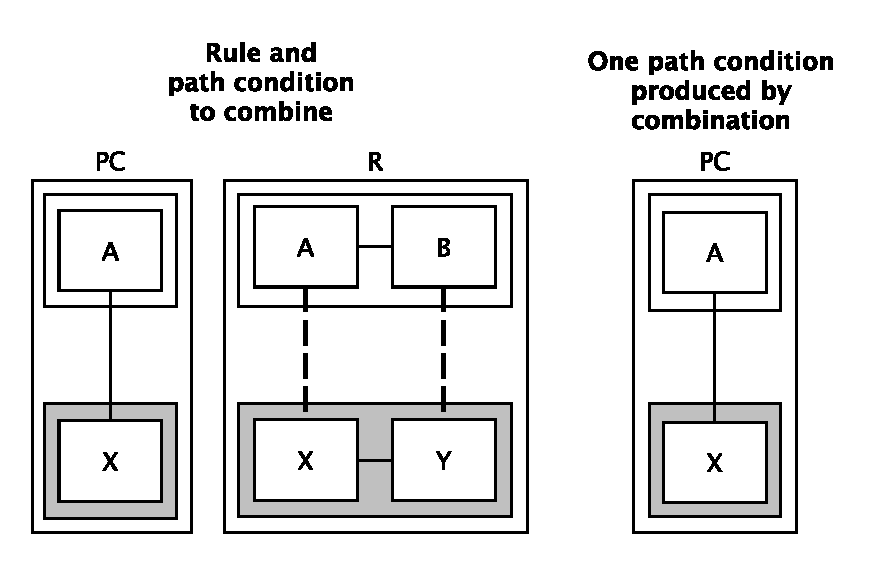
\includegraphics[width=0.44\textwidth]{./figures/building_path_conditions/non_satisfied_dependencies.pdf}
	\caption{R's dependencies are not satisfied by PC}
	\label{fig:non_satisfied_dependencies}
\end{figure}

\begin{definition}{Path Condition and Rule Combination -- Unsatisfied Dependencies\\} 
\label{def:rule_comb_unsatisfied}
\CatchFileBetweenTags{\unsatdeps}{text/definitions}{unsatdeps}{\unsatdeps}
\end{definition}

According to the pre-conditions of the equation presented in \cref{def:rule_comb_unsatisfied}, a path condition does not satisfy the dependencies present in a rule if there is no surjective typed graph homomorphism between the backward links of the rule and the symbolic traceability links of the path condition. Besides expressing the fact that all backward links must exist as symbolic traceability links the path condition, the surjective homomorphism allows modeling the case where dependencies expressed by two (or more) backward links between similarly typed elements can be satisfied by one single symbolic traceability link in the path condition \reviewer{Could be rephrased}. This is the case, for example, of rule \emph{FemaleToFemale} in the \emph{Police Station} in \cref{fig:dsltransformation}. The two similarly typed backward links in this rule are satisfied by a path condition containing only the rule \emph{females} generated from the first layer of the transformation, holding one single symbolic traceability link.


\paragraph{Partially- and Totally- Satisfied Dependencies}

Consider the possibility that the backward links of R can be found in PC, and R's dependencies are met. The question then becomes whether the rule R \textbf{may} or \textbf{will} execute in the abstracted transformation executions.

To resolve this question, the match graph of R, along with R's backward links, is matched to PC's match graph and traceability links. If all of these elements are found, then we denote this as the `totally-satisfied case', where R \textbf{will} necessarily execute in the abstracted transformation executions. Otherwise, we denote the `partially-satisfied' case, where R \textbf{may} execute. Note that we break up these cases for ease of explanation only. Formally, both cases are encompassed by \cref{def:rul_comb_partial_total}.

In the totally-satisfied case, R will be ``glued'' overtop PC, as seen in \cref{fig:total_satisfied_dependencies}. This gluing operation is anchored where the backwards links in R match over the traceability links in PC. The purpose of this operation is to include any elements in R's apply graph that may not exist in PC. Thus, all elements and associations which exist in both PC and R are ignored. Note that if multiple total matches exist in PC, that R will be glued at multiple points as seen in \cref{fig:multiple_total_satisfied_dependencies}. This ``gluing'' operation is also defined formally in \cref{def:rul_comb_partial_total}, as the addition of a delta graph.

\begin{figure*}[htb]
        \centering
        \begin{subfigure}[b]{0.7\textwidth}
                \centering
                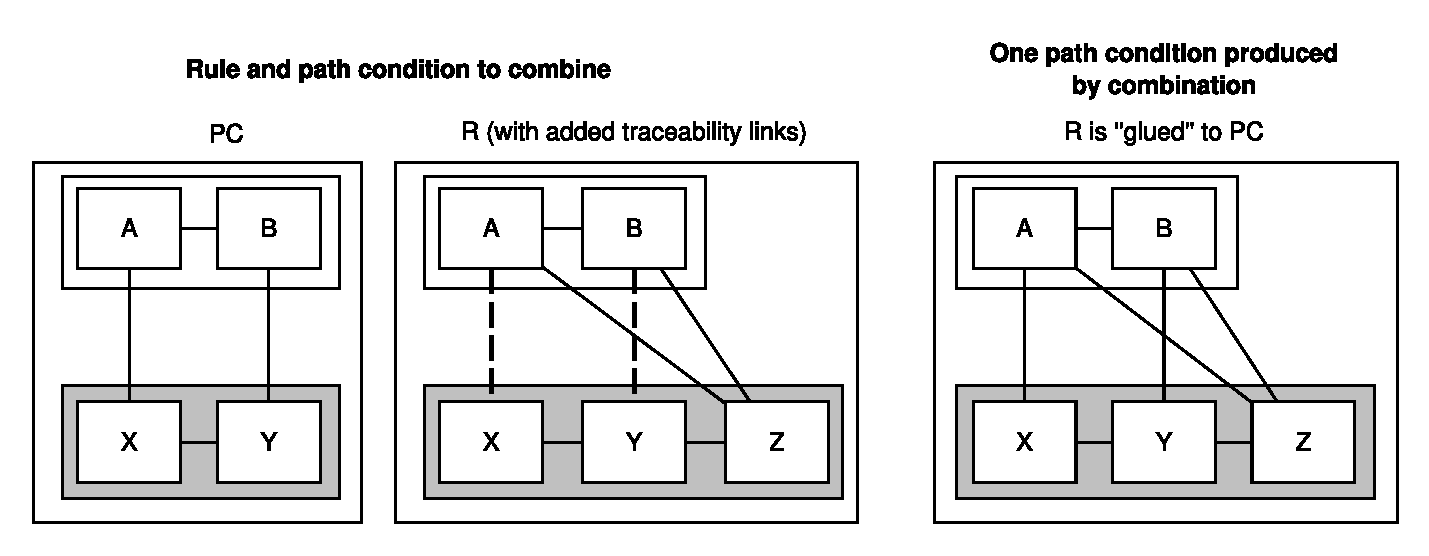
\includegraphics[width=1\textwidth]{./figures/building_path_conditions/total_satisfied_dependencies.pdf}
                \caption{Totally satisfied at one location}
                \label{fig:total_satisfied_dependencies}
        \end{subfigure}%
        \\
        \begin{subfigure}[b]{0.8\textwidth}
                \centering
                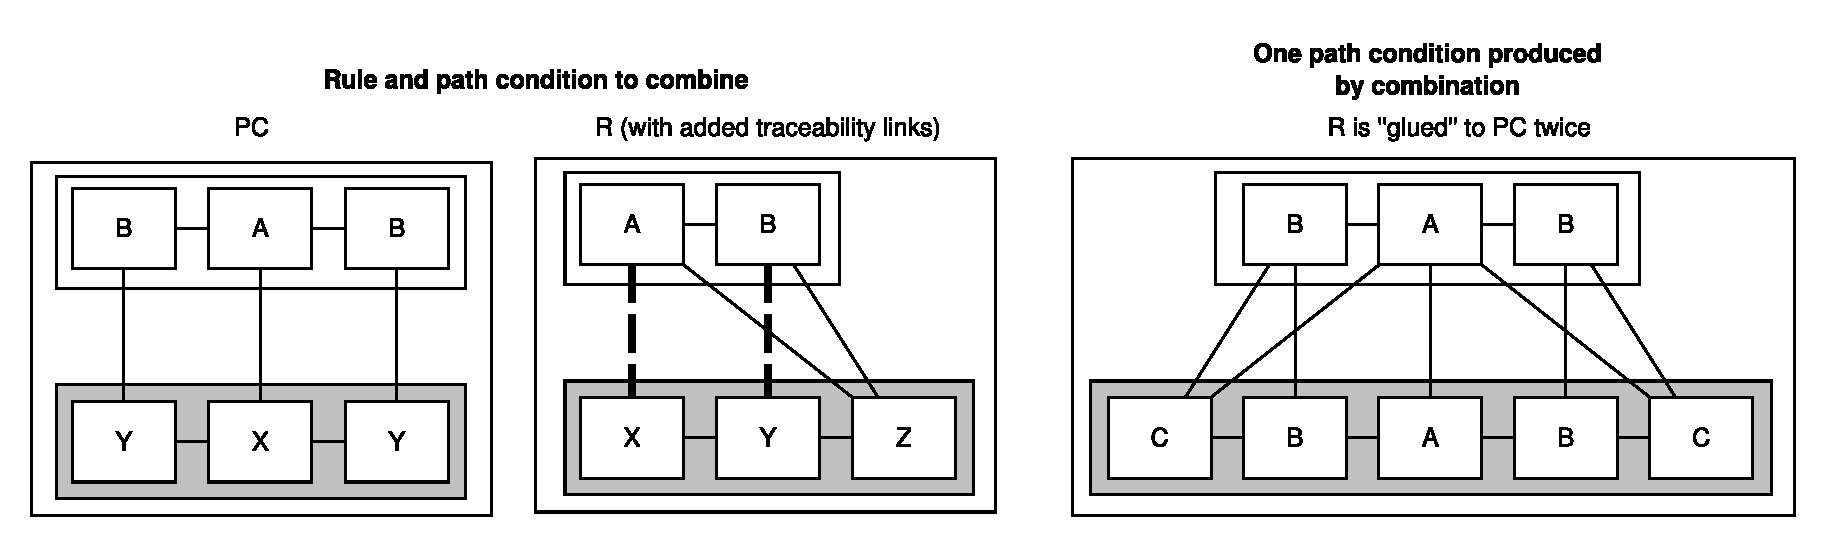
\includegraphics[width=1\textwidth]{./figures/building_path_conditions/multiple_total_satisfied_dependencies.pdf}
                \caption{Totally satisfied at multiple locations - \reviewer{Fix boxes on bottom}}
                \label{fig:multiple_total_satisfied_dependencies}
        \end{subfigure}%
        \caption{R's dependencies are totally satisfied by PC}
        \label{fig:totes_sat_deps}
\end{figure*}

In the partially-satisfied case, rule R may or may not execute. Note that in \cref{fig:partial_satisfied_dependencies}, PC does not have the association between the A and B elements in the match graph. This means that it is possible that the input model for the transformation does not have this association present. In these transformation executions R would not execute.
\cref{fig:partial_satisfied_dependencies} shows the two path conditions produced in this case. The first produced is a copy of PC, where R does not symbolically execute. The second is where R symbolically executes at the matched location. Therefore, R is glued onto PC, with the gluing step the same as in the totally-satisfied case above.

\begin{figure*}[tb] \centering 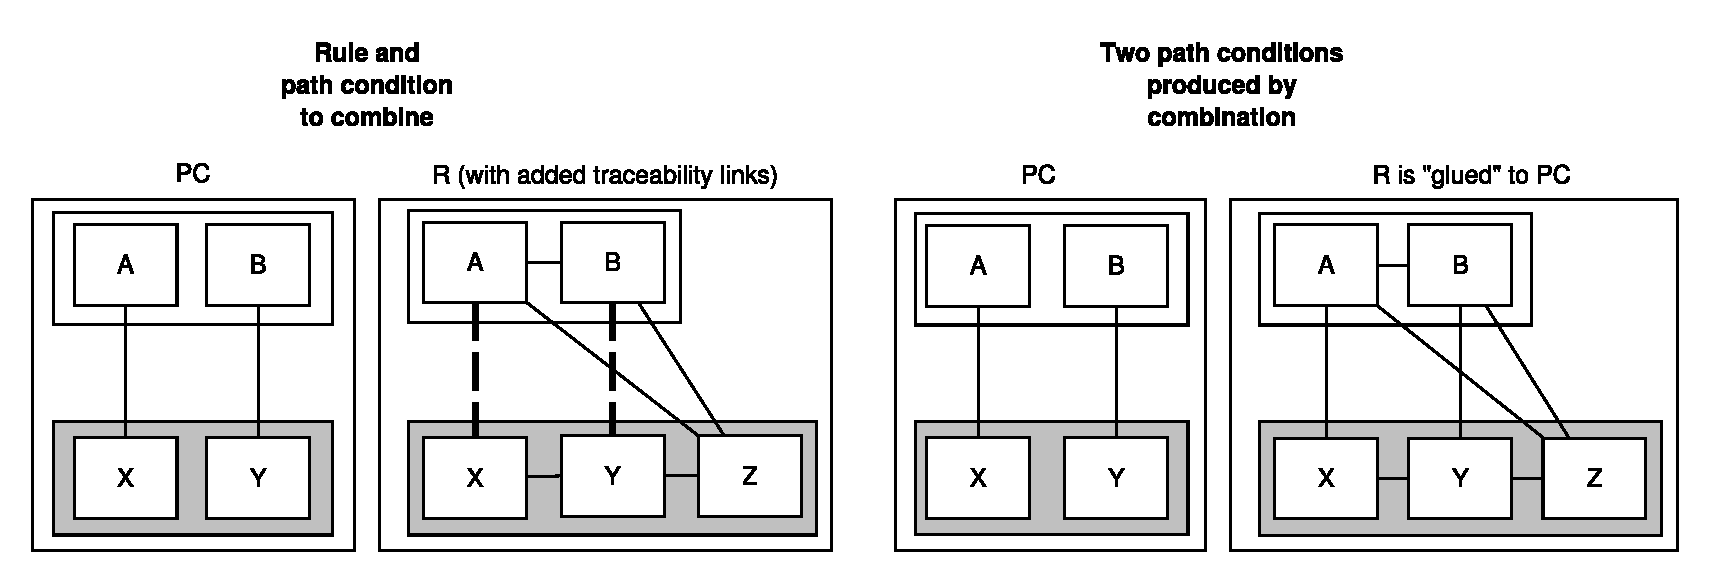
\includegraphics[width=0.8\textwidth]{./figures/building_path_conditions/partial_satisfied_dependencies.pdf}
	\caption{R's dependencies are partially satisfied by PC}
	\label{fig:partial_satisfied_dependencies}
\end{figure*}

Note that this gluing procedure must consider all matching possibilities, for each location the rule might match over the input model. For example, in \cref{fig:multiple_partial_satisfied_dependencies}, rule R has a backward link that can be partially matched on two locations in PC: the left-hand and right-hand pairs of traceability links. Therefore, there are four possibilities for how R would match over PC: not at all, on the left-hand side of PC, on the right-hand side, or on both sides. These four possibilities define the four new path conditions created.

The first is a copy of PC, as R is assumed to not execute and will produce no new elements. The second is where R will be glued on top of the backward links on the left-hand side, to add the elements that do not exist in PC already. The third is where the gluing will occur on the right-hand side. The fourth path condition produced is the case where R will be glued at both locations. 


\begin{figure*}[tb] \centering 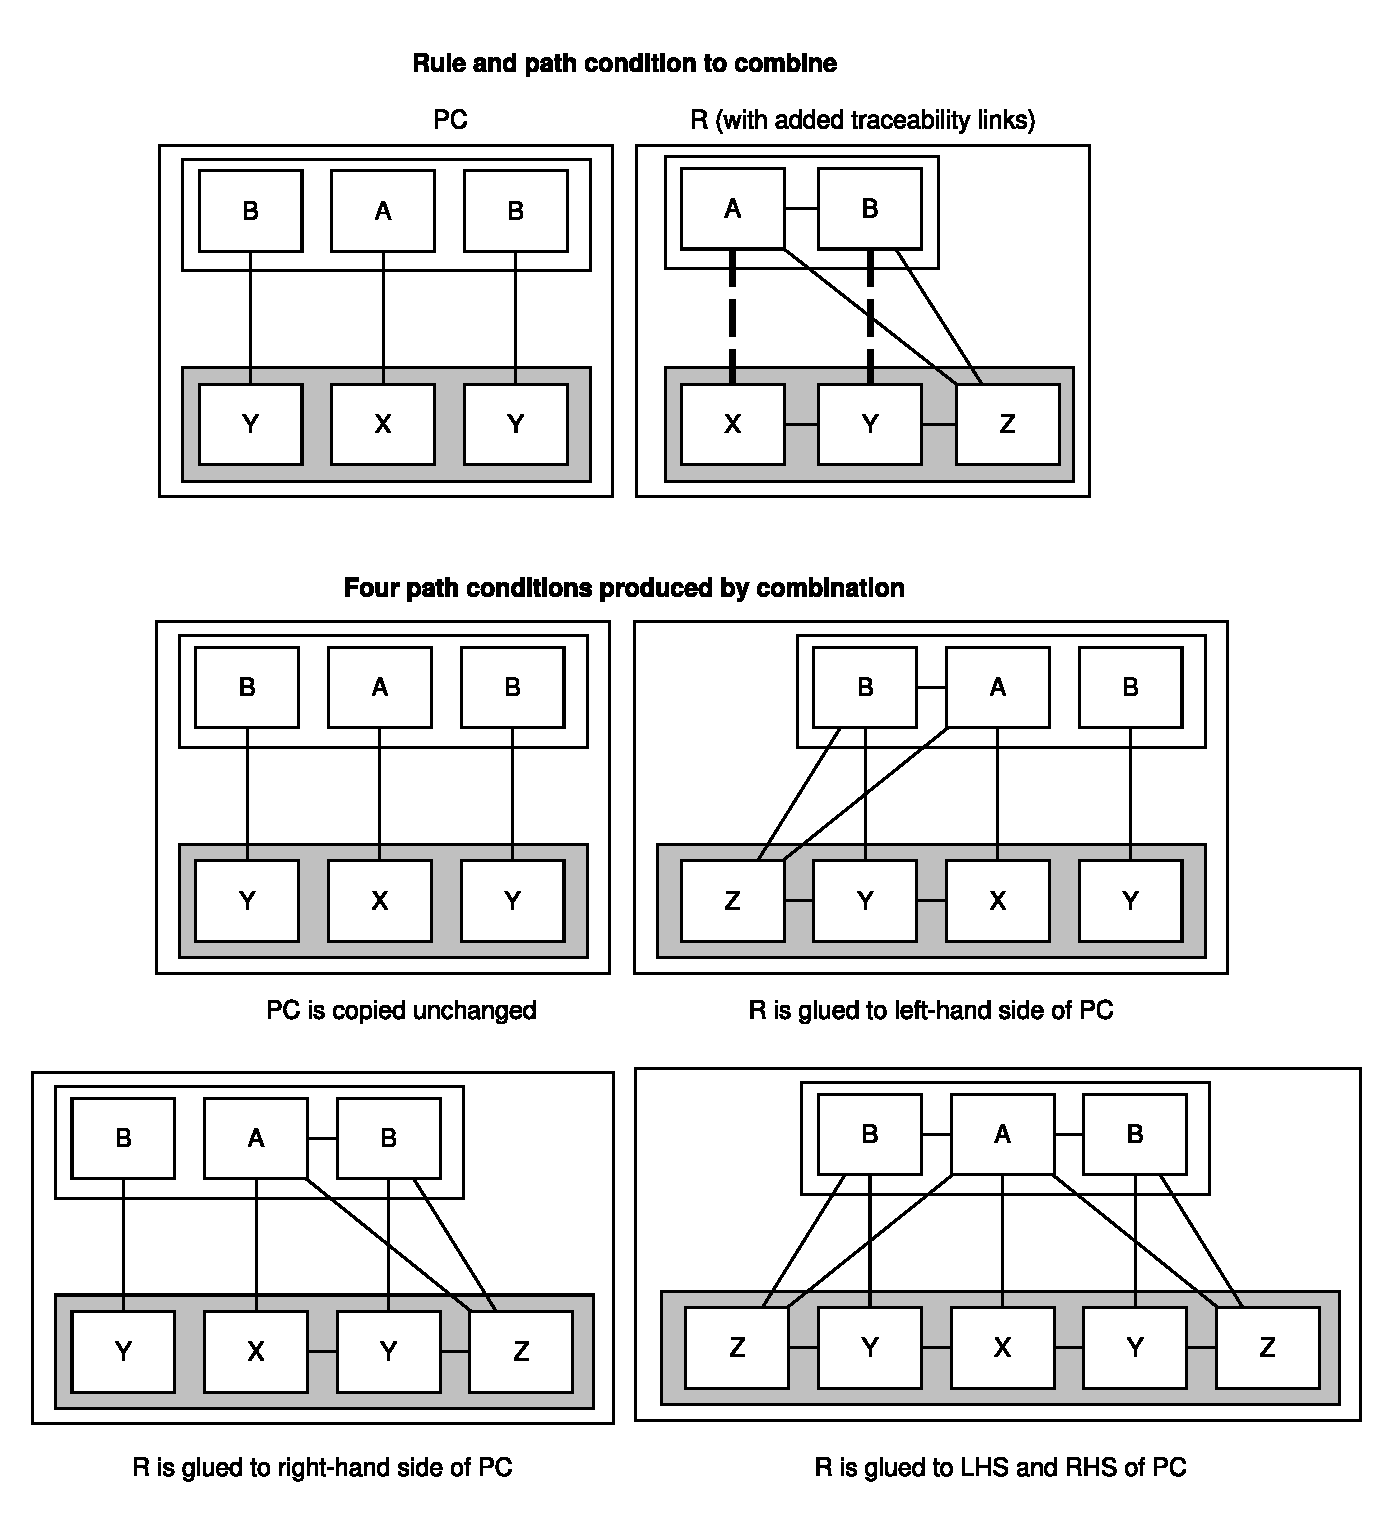
\includegraphics[width=0.8\textwidth]{./figures/building_path_conditions/multiple_partial_satisfied_dependencies.pdf}
	\caption{R's dependencies are partially satisfied by PC, and are glued at all possible matches}
	\label{fig:multiple_partial_satisfied_dependencies}
\end{figure*}


Note that rules may also contain transitive links in their match graphs. In this case, the partial or total matching of R onto PC must consider all transitive matches in order to produce all valid path conditions.

As we have done for the previous cases, let us now formally define the combination step when a rule has partially and/or totally defined dependencies. As these cases are more complex than the previous two, we will need to construct the mathematical model of this case incrementally. We will start by an auxiliary relation that partially or totally combines a set of path conditions with a rule.

\begin{definition}{Single Partial and Total Combination of a Set of Path Conditions with a Rule\\}
\label{def:comb_path_cond_rule_single}
\CatchFileBetweenTags{\satdeps}{text/definitions}{satdeps}{\satdeps}

\begin{align}
\label{eq:pcomb}
\CatchFileBetweenTags{\satdepseqone}{text/definitions}{satdepseqone}{\satdepseqone}
\end{align}


\begin{align}
\label{eq:tcomb}
\CatchFileBetweenTags{\satdepseqtwo}{text/definitions}{satdepseqtwo}{\satdepseqtwo}
\end{align}

\end{definition}


Let us start by introducing relation $\stackrel{p\_comb}{\rightarrow}$, presented in \cref{eq:pcomb} of \cref{def:comb_path_cond_rule_single}. The relation takes as arguments a set of path conditions being accumulated for the current layer, the rule to be combined, and an $rl_{glue}$ argument indicating the place in each of the input path conditions the rule should be anchored to during the combination step. The relation's output is a new set of path conditions. This new set includes all the original path conditions, as well as each path condition in the accumulator set ``glued'' to a copy of rule being examined. Note that the relation $\stackrel{t\_comb}{\rightarrow}$ in \cref{eq:tcomb} of \cref{def:comb_path_cond_rule_single} is similarly defined, except for the fact path conditions in the accumulator set are not preserved in the relation's output set.\\

\setcounter{equation}{0} 

Let us now define how a rule is combined with a path condition, whenever its backward links can be found several times in that path condition. This situation is described in the examples in \cref{fig:multiple_total_satisfied_dependencies} and \cref{fig:multiple_partial_satisfied_dependencies}. We formalize it in \cref{def:comb_path_cond_rule_mul}, by means of relations $\stackrel{p\_step}{\rightarrow}$ and $\stackrel{t\_step}{\rightarrow}$. These two relations operationally describe the sequence of steps necessary to ``glue'' a rule at multiples places of a path condition. The set of places targeted in the path condition for receiving a copy of the rule is given by the sets $partialSet$ and $totalSet$ (found respectively in Equation~(2) and Equation~(4) of \cref{def:comb_path_cond_rule_mul}). As expected, these sets contain the set of traceability links in the path condition where copies of the rule need to be anchored to.

\begin{definition}{Multiple Partial and Total Combination of a Set of Path Conditions with a Rule\\}
\label{def:comb_path_cond_rule_mul}

\CatchFileBetweenTags{\satdepstwo}{text/definitions}{satdepstwo}{\satdepstwo}
\end{definition}

Having \cref{def:comb_path_cond_rule_single} and \cref{def:comb_path_cond_rule_mul} in mind, we can now proceed to define the complete combination relation of a rule with a path condition in the case of partially and totally satisfied dependencies. 

\begin{definition}{Path Condition and Rule Combination -- Partially and Totally Satisfied Dependencies\\}
\label{def:rul_comb_partial_total}

\CatchFileBetweenTags{\satdepsthree}{text/definitions}{satdepsthree}{\satdepsthree}
\end{definition}

The top equation in \cref{def:rul_comb_partial_total} defines the $\stackrel{combine}{\rightarrow}$ relation for when rule $rl$ has dependencies that are satisfied by path condition $pc$. The pre-conditions in the equation state that the backward links in the rule are found in the path condition, as expected. Additionally, two sequential steps perform the gluing of the rule $rl$ on all path conditions in accumulator $AC$, wherever the rule is partially and/or totally found in each of those path conditions. Relations $\stackrel{p\_comb}{\rightarrow}$ and $\stackrel{t\_comb}{\rightarrow}$ presented in \cref{def:comb_path_cond_rule_mul} are used to model these two operational ``gluing'' steps. Functions $partialsat$ and $totalsat$, described in the latter part of \cref{def:rul_comb_partial_total}, are used to gather the places of path condition $pc$ where copies of the rule need to be anchored to.


\subsubsection{Considering Further Rules}
\label{sec:further_rules}
Thus far we have described how to create a set of path conditions that represent how one rule from a layer will add new elements to one path condition from the previous layer. These path conditions are then themselves combined with the next rule in the layer in the same manner. Note that in \cref{def:rul_comb_partial_total} the choice of next rule does not matter, due to the rule non-interference guaranteed by the semantics of DSLTrans. In order to represent this non-interference in the construction of path conditions, we specify that the matching of rule dependencies is against the path condition from the previous layer (variable $pc$ in the main equation of \cref{def:rul_comb_partial_total}), not the specific path condition the rule is to be combined with in the accumulator argument of the $\stackrel{combine}{\rightarrow}$ relation. This ensures that the result of combining one rule with a path condition will have no impact on how following rules will combine.

% Note that the choice of next rule does not matter, due to the rule non-interference guaranteed by the semantics of DSLTrans. In order to represent this non-interference in the construction of path conditions, we specify that the matching of rule dependencies is against the path condition from the previous layer, not the specific path condition the rule is to be combined with. This ensures that the result of combining one rule with a path condition will have no impact on how following rules will combine.

The combination of one path condition with all the rules in the layer will produce a new set of path conditions. This process is depicted in \cref{fig:all_pcs2} and formalized in \cref{def:path_cond_layer_comb} by the layer combination relation $\stackrel{combpclayer}{\rightarrow}$.

\begin{definition} {Combining a Path Condition with a Layer\\}
\label{def:path_cond_layer_comb}
\CatchFileBetweenTags{\combpclayer}{text/definitions}{combpclayer}{\combpclayer}
\end{definition}

\CatchFileBetweenTags{\combpclayertext}{text/definitions}{combpclayertext}{\combpclayertext}

\begin{definition} {Combining a Set of Path Conditions with a Layer\\}
\label{def:path_cond_set_layer_comb}
\CatchFileBetweenTags{\combpcsetlayer}{text/definitions}{combpcsetlayer}{\combpcsetlayer}
\end{definition}

\CatchFileBetweenTags{\combpcsetlayertext}{text/definitions}{combpcsetlayertext}{\combpcsetlayertext} 

\begin{definition} {Path Condition Generation\\}
\label{def:path_cond_gen}
\CatchFileBetweenTags{\pathcondgen}{text/definitions}{pathcondgen}{\pathcondgen}
\end{definition}

\CatchFileBetweenTags{\pathcondgentext}{text/definitions}{pathcondgentext}{\pathcondgentext} 






\section{Validity and Completeness}
\label{subsec:abstraction_relation_validity_completeness}

This section presents our arguments that our path condition building
algorithm is both \emph{valid} and \emph{complete}. In this context
\emph{validity} means that for each path condition there exists at least one
transformation execution that it abstracts.
In other words, no path conditions are produced that lack a concrete
transformation execution counterpart. \emph{Completeness} of the symbolic
execution means that every transformation execution is abstracted by at least
one path condition.

%\newpage
\begin{proposition}{(Validity)}
\label{prop:pc_validity}
Every path condition abstracts at least one transformation execution.
\end{proposition}
\begin{ps}

Let $tr\in \textsc{Transf}^{sr}_{tg}$ be a DSLTans transformation. We wish to demonstrate that, for all path conditions $pc\in \textsc{Pathcond}(tr)$, there exists a transformation execution $ex\in \textsc{Exec}(tr)$ of the set of
rules used to build $pc$ such that $pc$ abstracts $ex$, as formally expressed in \cref{def:abstraction_pc_ex}. We can prove this property by induction on the set of transformations $\textsc{Transf}^{sr}_{tg}$ (see \cref{def:layer_transformation}), as follows:

\begin{itemize}
  \item \emph{Base case:} the base case is when $tr$ is the empty
  transformation. In this case, according to \cref{def:path_cond_gen} only the
  empty path condition $\epsilon_{pc}$ exists in the path condition set. We thus
  need to demonstrate that the empty path condition abstracts the empty
  transformation execution $\epsilon_{ex}$, as well as any execution for which
  the input model is never matched by any rule (consequently having an empty
  output model). For any of these transformation executions, Proposition~\ref{eq:abstr_input_output} of the abstraction relation definition is satisfied, as no rule copy exists in the path condition and the output of the transformation execution is empty -- empty typed graph homomorphisms thus satisfy all the conditions of the proposition. Proposition~\ref{eq:abstr_trace} of the abstraction relation definition also trivially holds because no traceability links exist either in the path condition or in any of the considered executions.
  
%   This is so because:
%   1) the empty typed graph homomorphism is an injective typed graph homomorphism
%   between the match part of the empty path condition and any input model; and 2) as
%   well as a surjective typed graph homomorphism between an empty output model
%   and the apply part of the empty path condition.
 
   \item \emph{Base case:} the base case is the case when we have $tr=[\;]$, i.e. the empty transformation. In this case, according to \cref{def:path_cond_gen_appendix}, only the empty path condition $\epsilon_{pc}$ exists in the path condition set. The empty path condition abstracts the empty transformation execution $\epsilon_{ex}$ (see \cref{def:modeltransformation_appendix}), as well as any execution for which the input model is never matched by any rule (consequently having an empty output model). For any of these transformation executions, \cref{eq:abstr_input_output} of the abstraction relation definition is satisfied, as: a) no rule copy exists in the path condition and the output of the transformation execution is empty -- empty typed graph homomorphisms thus satisfy the all the conditions of the proposition; and b) \cref{eq:abstr_trace} of the abstraction relation definition trivially holds because no traceability links exist either in the path condition or in any of the considered executions.
   
\item \emph{Inductive case:} assuming every path condition generated for a transformation $tr$ abstracts at least one transformation execution, we need to show that every path condition generated for a transformation $tr'$, resulting from adding a layer $l\in \textsc{Layer}^{sr}_{tg}$ to $tr$, will also abstract at least one transformation execution. 
\end{itemize}

In order to demonstrate the inductive case we need to show the property holds for all path conditions resulting from combining the rules of layer $l$ with any path condition generated for $tr$. These path conditions for transformation $tr'$ are built as expressed in \cref{def:path_cond_layer_comb}. According to this definition, path conditions for $tr'$ are built by incrementally combining the path conditions generated for $tr$ with a rule of layer $l$, until all the rules in $l$ have been treated. We can thus again use induction for this proof, this time on the set of possible layers $\textsc{Layer}^{sr}_{tg}$. 

\begin{itemize}
  \item \emph{Base case:} this is the case where layer $l$ contains no rules. In this case, by the base case of \cref{def:path_cond_layer_comb}, no new path condition is added to the set of path conditions generated for the transformation $tr$. As such the $tr=tr'$ and by induction hypothesis the property trivially holds for all path conditions generated for $tr'$.
  
  \item \emph{Inductive case:} for the inductive case (transitive case of \cref{def:path_cond_layer_comb}) we need to show that, assuming the property holds for all path conditions generated for a transformation $tr$, then the property will also hold for a transformation $tr'$ -- where $tr'$ results from adding a new rule $rl$ to the last layer of $tr$. We will thus need to consider the four \reviewer{three?} cases of rule combination:\vspace{.2cm} 
 
\begin{enumerate}
\item\label{lab:rule_case1} Rule $rl$ has no dependencies (\cref{def:rule_comb_no_dependencies}).
\item\label{lab:rule_case2} Rule $rl$ has dependencies and cannot execute (\cref{def:rule_comb_unsatisfied}).
\item\label{lab:rule_case3} Rule $rl$ has dependencies and may and/or will execute (\cref{def:rul_comb_partial_total}).
\end{enumerate}

The property trivially holds for case~\ref{lab:rule_case2}, given that no new path conditions are added to the path condition set generated for $tr$ and that the property holds for $tr$ by induction hypothesis. When a rule $rl$ is added to the last layer of $tr$ such that cases~\ref{lab:rule_case1} or~\ref{lab:rule_case3} occur, then the property can be shown to hold for $tr'$ as follows: 1) choose for a general path condition $pc$ generated for $tr$ an execution $ex$ such that $pc$ abstracts $ex$; 2) build an input model $m$ as the result of uniting the input model of $ex$ with a model that can be matched by $rl$; 3) execute $tr'$ having as input model $m$ to produce transformation execution $ex'$; and finally 4) demonstrate $ex'$ is abstracted by the path condition $pc'$ resulting from combining $pc$ with $rl$ whether rule $rl$ does not depend on $pc$ or rule $rl$ depends on $pc$ and may and/or will execute.

The property trivially holds for case~\ref{lab:rule_case2_appendix}, given that no new path conditions are added to the path condition set generated for $tr$ and that the property holds for $tr$ by induction hypothesis.

When a rule $rl$ is added to the last layer of $tr$ such that cases~\ref{lab:rule_case1_appendix} or~\ref{lab:rule_case3_appendix} occur, new path conditions are added to the path condition set. Both cases are based on combining a path condition with a rule, as laid out in \cref{def:combine_pc_with_rule_appendix}. In order to demonstrate this second inductive step we then need to show that, whenever the property holds for a path condition $pc$ generated for a transformation $tr$, the combination of $pc$ with a rule $rl$ results in a new path condition where the property is respected.

We start by picking for $pc$ an execution $ex$ such that $pc$ abstracts $ex$. We know such a transformation execution exists by induction hypothesis. We can then build an input model $m$ as the result of uniting the input model of $ex$ with a model that can be matched by $rl$. If we execute $tr'$ having $m$ as input model we obtain transformation execution $ex'$.

Let us now demonstrate $ex'$ is abstracted by the path condition $pc'=pc\stackrel{trace}{\sqcup} rl$, the combination of $pc$ with $rl$ as shown in \cref{def:combine_pc_with_rule_appendix}. We first recall the conditions of the abstraction relation in \cref{def:abstraction_pc_ex_appendix}:
\begin{enumerate}
	\item\label{item:abstr_rel1} a) injective typed graph homomorphisms must exist between the match parts of all the rule copies in the path condition and the input of the execution \emph{and} b) a surjective typed graph isomorphism must exist between the output of the execution and the apply part of the path condition.
    \item\label{item:abstr_rel2} a) injective typed graph homomorphisms must exist between all strongly connected components of the path condition composed of only symbolic traceability links \emph{and} b) all isolated traceability links in the transformation execution must be found at least once in the path condition.\vspace{.3cm}
\end{enumerate} 

Let us start by arguing for why condition~\ref{item:abstr_rel1} a) holds for $pc'$ and $ex'$. Because we know rule $rl$ has executed on the input model of $ex'$, we know by \cref{def:match_function} of the function matching a DSLTrans rule that an injective typed graph homomorphism exists between the match part of $rl$ and $ex'$. When $rl$ is combined with $pc$, its match part is preserved in $pc$ and as such an injective typed graph homomorphism must exist between it and $ex'$. By induction hypothesis and because the combination operator is additive (meaning nothing existing in $pc$ is deleted during combination) we know injective typed graph homomorphisms continue to exist between the match parts of all other rule copies in the path condition and the input of the $ex'$.\vspace{.3cm}

In what concerns condition~\ref{item:abstr_rel1} b) above, we know by \cref{def:apply_function} and \cref{def:layer_step_semantics} that one or more copies of graphs isomorphic to the apply part of $rl$ are added to the output of $ex$. Also, by \cref{def:layer_step_semantics}, we know this addition preserves the output of $ex$ and we also know by hypothesis that a surjective typed graph isomorphism exists between the output of $ex$ and the apply part of $pc$. As mentioned before, the combination of $pc$ and $rl$ is additive and as such we can also deduce that a typed graph isomorphism exists between the apply part of any copy $rl$ added to $ex$ and the apply part of $rl$ added to $pc$. As such, all old and new edges and nodes in $ex'$ can be surjectively found in $pc'$.\vspace{.3cm}

We will now discuss the reasons why condition~\ref{item:abstr_rel2} a) of the abstraction relation holds for $pc'$ and $ex'$. When $pc$ and $rl$ are combined, by \cref{def:combine_pc_with_rule_appendix} a copy of the rule is ``glued'' on top of $pc$. Symbolic traceability links are added between elements of the match part of the copy of the rule and of the apply copy of the rule, for those elements in the apply part of the copy of the rule not previously connected to backward links. We also know by \cref{def:apply_function} that traceability links are similarly added to the copy of $rl$ that is merged with $ex$. Because of the induction hypothesis we know that injective typed graph homomorphisms exists between all the strongly connected components composed of traceability links of $pc$ and $ex$. When $rl$ is combined with $pc$ two cases can occur: a) $rl$ has no backward links, in which the proposition trivially holds because isomorphic isolated strongly connected components are added both to $pc$ and $ex$; b) $rl$ has backward links, in which case the newly added components will connect to existing strongly connected components in $pc$ and $ex$, forming additional strongly connected components. In this case, an injective typed graph homomorphism exists between each of the newly formed strongly connected components in $pc$ and at least one newly formed strongly connected component in $ex$. This is so because, by \cref{def:abstraction_pc_ex_appendix} of the abstraction relation between a path condition and a transformation execution, the set of rules combined into $pc$ and the set of rules that have executed is the same. The combination of these rules in the path condition, according to \cref{def:combine_pc_with_rule_appendix}, replicates patterns that are produced in the execution by \cref{def:apply_function} and \cref{def:layer_step_semantics}. Note that condition~\ref{item:abstr_rel2} a) of the abstraction relation provides additional guarantee that, when multiple partially and/or totally satisfied dependencies occur during path condition combination (\cref{def:rul_comb_partial_total_appendix}), the corresponding executions are correctly abstracted given each place where the rules are ``glued'' corresponds to a different strongly connected component.\vspace{.3cm}
 
Condition~\ref{item:abstr_rel2} b) of the abstraction relation trivially holds as each new traceability link added to $ex$ when $rl$ executes has at least one corresponding symbolic traceability link in $pc'$, resulting from the combination of $pc$ with $rl$.  

\end{itemize}
\end{ps} 


\begin{proposition}{(Completeness)}
\label{prop:pc_completeness}
Every transformation execution is abstracted by one path condition.
\end{proposition}
\begin{pf}
Let $tr\in \textsc{Transf}^{sr}_{tg}$ be a DSLTans transformation. We wish to demonstrate that, for all transformation executions $ex\in \textsc{Exec}(tr)$, a path condition $pc\in \textsc{Pathcond}(tr)$ exists such that $ex$ is abstracted by $pc$, as formally expressed in \cref{def:abstraction_pc_ex}.\\ 

Completeness can be shown as a corollary of \cref{prop:pc_validity} about the \emph{validity} of path condition generation. The complete set of executions $\textsc{Exec}(tr)$ (see \cref{def:modeltransformation}) can be split into two kinds of executions:
\begin{enumerate}
  \item\label{lab:input_not_matched} The \emph{empty execution} $\epsilon_{ex}$ or the \emph{execution where the input model was not matched by any rule}. As mentioned in \cref{prop:pc_validity}, these executions are abstracted by the empty path condition $\epsilon_{pc}$.\vspace{.3cm}
  \item The \emph{execution $ex$ where a number of rules of $tr$ have been applied to the input model}, where each transformation rule $rl$ of $tr$ may have been applied more than once. In this case we have that, because all possible and valid rule combinations are considered when building path conditions, a path combination $pc$ exists that contains one or more copies of each of the rules used when operationally building $ex$. \\
  
  Moreover, during the proof of \emph{validity} of path condition generation in \cref{prop:pc_validity} we demonstrate that, when we add a new rule $rl$ to the last layer of a transformation $tr$ (such that we have a new transformation $tr'$), the rule combination step explained in Definitions~\ref{def:rule_comb_no_dependencies},~\ref{def:rule_comb_unsatisfied} and~\ref{def:rul_comb_partial_total} produces a new set of path conditions where each path condition in that set still abstracts at least one transformation execution of $tr'$. This part of the proof (the second induction) is achieved by building for transformation $tr'$ an input model $m$ that can be matched by $rl$ (as well as by all the other rules of $tr$), and then building from $m$ a new transformation execution that is abstracted by a path condition built for $tr'$. Because in the proof of \cref{prop:pc_validity}, $m$ is such that it can be matched by $rl$ an arbitrary amount of times, we know that, independently of the number of times a rule is applied during the construction of a transformation execution, a path condition abstracting that transformation execution exists.\\

Additionally, input elements that are not matched by any rule do not affect the abstraction relation, as explained in case~\ref{lab:input_not_matched} above. This means we also know that executions involving input models that are only partially matched by the rules of $tr$ are also abstracted by one path condition. 
\end{enumerate}

Let $tr\in \textsc{Transf}^{sr}_{tg}$ be a DSLTans transformation. We wish to demonstrate that, for all transformation executions $ex\in \textsc{Exec}(tr)$, a path condition $pc\in \textsc{Pathcond}(tr)$ exists such that $ex$ is abstracted by $pc$, as formally expressed in \cref{def:abstraction_pc_ex_appendix}.
Completeness can be shown as a corollary of \cref{prop:pc_validity_appendix} about the \emph{validity} of path condition generation. The complete set of executions $\textsc{Exec}(tr)$ (see \cref{def:modeltransformation_appendix}) can be split into two kinds of executions:
\begin{enumerate}
  \item\label{lab:input_not_matched} The \emph{empty execution} $\epsilon_{ex}$ or the \emph{execution where the input model was not matched by any rule}. As mentioned in \cref{prop:pc_validity_appendix}, these executions are abstracted by the empty path condition $\epsilon_{pc}$.\vspace{.3cm}
  \item The \emph{execution $ex$ where a number of rules of $tr$ have been applied to the input model}, where each transformation rule $rl$ of $tr$ may have been applied more than once. In this case we have that, because all possible and valid rule combinations are considered when building path conditions, a path combination $pc$ exists that contains one or more copies of each of the rules used when operationally building $ex$. 
Moreover, during the proof of \emph{validity} of path condition generation in \cref{prop:pc_validity_appendix} we demonstrate that, when we add a new rule $rl$ to the last layer of a transformation $tr$ (such that we have a new transformation $tr'$), the rule combination step explained in Definitions~\ref{def:rule_comb_no_dependencies_appendix},~\ref{def:rule_comb_unsatisfied_appendix} and~\ref{def:rul_comb_partial_total_appendix} produces a new set of path conditions where each path condition in that set still abstracts at least one transformation execution of $tr'$. This part of the proof (the second induction) is achieved by building for transformation $tr'$ an input model $m$ that can be matched by $rl$ (as well as by all the other rules of $tr$), and then building from $m$ a new transformation execution that is abstracted by a path condition built for $tr'$. Because in the proof of \cref{prop:pc_validity_appendix}, $m$ is such that it can be matched by $rl$ an arbitrary amount of times, we know that, independently of the number of times a rule is applied during the construction of a transformation execution, a path condition abstracting that transformation execution exists.\\

Additionally, input elements that are not matched by any rule do not affect the abstraction relation, as explained in case~\ref{lab:input_not_matched} above. This means we also know that executions involving input models that are only partially matched by the rules of $tr$ are also abstracted by one path condition. 
\end{enumerate} 
\end{pf} 

% Our path conditions construction algorithm takes all possible interactions of rules
% into account:
% \begin{enumerate}
% \item When building the path conditions for one layer we have built all
% the combinations of rules, as well as their possible interactions through
% \emph{disambiguation};
% \item When combining the path conditions from different layer different layers
% we have considered the cases where no interactions exist, or where backward
% links in rules requires certain certain elements to already exist in the
% generated model thus far.
% \end{enumerate}
% Note that, given the considered subset of DSLTrans constructs as described
% in \cref{sec:dsltrans}, no additional cases of rule interaction other than the
% ones described above need to be considered.
% From \cref{prop:pc_validity} we also know that at least one concrete
% transformation execution exists per path condition. In the proof of
% \cref{prop:pc_validity} we have built, for each path condition $A$,
% the simplest transformation execution that is abstracted by $A$. These
% transformation executions produce one instance of each element and association
% present in the apply pattern of $A$. However, given
% \cref{def:instance_pc_ex} in \cref{sec:proofs} (abstraction of
% a transformation execution by a path condition), an infinite amount of
% transformation executions are always abstracted by $A$. These executions
% correspond to the generation of output models holding an arbitrarily large
% amount of the elements and associations while still being abstracted by $A$.
% Because we have considered all possibilities of execution in our path condition
% construction algorithm, the union of all transformation executions built for
% each path condition constitutes the complete, infinite set of transformation
% executions. We thus know that every possible transformation execution is
% abstracted by at least one path condition.


% Note that we do not provide any guarantee that the same transformation execution
% cannot be abstracted by two different path conditions. Although given our symbolic
% execution assumptions we believe this to be the case, further mathematical
% exploration of this issue is necessary. Given however the fact that our
% verification algorithm exhaustively explores all path conditions, it is
% sufficient for the property proof to provide a \emph{no} result in the analysis
% of a path condition for the result of the verification of the property to be
% \emph{no}. \levi{keep this?}

\begin{lemma} (Uniqueness) 
\label{lem:uniqueness}
A transformation execution is abstracted by exactly one path condition.
\end{lemma}
\begin{ps}
Let $tr\in \textsc{Transf}^{sr}_{tr}$ be a model transformation. We will demonstrate that two different path conditions\\$pc_1, pc_2\in \textsc{Pathcond}(tr)$ cannot exist such that we have a transformation execution $ex\in \textsc{Exec}(tr)$ where $ex\Vvdash pc_1$ and $ex\Vvdash pc_2$.

We will do so by attempting to build an $ex\in \textsc{Exec}(tr)$ such that $ex\Vvdash pc_1$ and $ex\Vvdash pc_2$ and demonstrating that it is always the case that such is not possible. In order to structure our argumentation, we will consider two cases:
% \levi{the contradiction happens because at each point of the execution, when a rule is added any two path conditions from the existing set of path conditions will represent different executions. At all points if we consider two path conditions in the PC set we have that two different executions can be created if we find a model that satisfies the first condition of the abstraction relation, and it is always the case that none of those two executions can be abstracted by the two path conditions simultaneously.}
\begin{enumerate}
  \item\label{item:uniqueness_rule_no_dep} the case where no rules in $tr$ have dependencies.
  \item\label{item:uniqueness_rule_has_dep} the case where some rules in $tr$ have dependencies.
\end{enumerate}

We start by considering that $tr$ falls into case~\ref{item:uniqueness_rule_no_dep} above. By~\cref{def:path_cond_gen} of path condition generation, each rule appears at most once in a path condition. Also, by construction, each path condition always contains a different combination of rules. We additionally know from \cref{def:layer_transformation} that the rules that compose $tr$ necessarily have non-overlapping matchers. We can nonetheless build a model $m$ as the typed graph union of two input models $m_1$ and $m_2$, where injective typed graph morphisms can be found between the match parts of the rule copies that form $pc_1$, and $m_1$. Injective typed graph morphisms can be found as well between the match parts of the rules that form $pc_2$, and $m_2$. We thus know that injective typed graph morphisms can be found between the rule copies that compose $pc_1$ and $pc_2$, and $m$. This satisfies the first condition of \cref{eq:abstr_input_output} in ~\cref{def:abstraction_pc_ex} of abstraction relation. 

Let us now consider that $ex_1$ and $ex_2$ are obtained by executing the transformations rules combined into $pc_1$ and $pc_2$, having $m$ as input model. As mentioned above, we know that the rules in $pc_1$ and $pc_2$ are not completely overlapping. This means that, due to the way in which $m$ is built (explained above), $m$ will always have at least one input that is matched by rules of $pc_1$ but not by rules of $pc_2$ (and vice-versa). Thus, when the transformation rules combined into $pc_1$ execute having $m$ as an input model, there will always exist a traceability link generated between an input and an output element of $m$ that is not generated when the transformation rules combined into $pc_2$ execute having $m$ as an input model (and vice-versa). As such, we have that $ex_1$ is always different from $ex_2$ by at least one traceability link. Given that this traceability link is symbolically represented in either $pc_1$ or $pc_2$ (but not in both), according to condition \cref{eq:abstr_trace} in \cref{def:abstraction_pc_ex_appendix} it cannot be that either $pc_1$ or $pc_2$ abstract $ex_1$ and $ex_2$ simultaneously.\\\\
We will now analyse the scenario where $tr$ falls into case~\ref{item:uniqueness_rule_has_dep_appendix} above, where some rules in $tr$ have dependencies. For this case, assume we have a path condition $pc_1$ contained in the set of path conditions generated for $tr$, considering layers up to layer $l$ of $tr$ have executed. Assume also we have a rule $rl$ of layer $l+1$ of $tr$ that has dependencies and can be combined with $pc$. If rule $rl$ is totally combined with path condition $pc_1$, according to \cref{def:rul_comb_partial_total_appendix} and \cref{fig:multiple_total_satisfied_dependencies}, then nothing needs to be shown as $pc_1$ is not kept in the path condition set but rather replaced by its combination with $rl$. However, in case rule $rl$ is partially combined with $pc$, as defined in \cref{def:rul_comb_partial_total_appendix} and \cref{def:comb_path_cond_rule_single_appendix}, then multiple path conditions are generated and additionally $pc_1$ is kept in the path condition set. Consider $pc_2$ is one of the newly created path conditions. In this case we can find a model $m$ that can be injectively matched by the rule copies in both $pc_1$ and $pc_2$: $m$ is the union of the input model isomorphic to the match part of $pc_1$, united with the input model isomorphic to the match part of $pc_2$ (including symbolic traceability links).\vspace{.3cm}

As before, we now consider that $ex_1$ and $ex_2$ are obtained by executing the rules used to build $pc_1$ and $pc_2$, respectively, having $m$ as input model. In this case, we have that either $rl$ was ``glued'' across different rule copies in $pc_2$, or over one single rule copy of $pc_2$. In the first case, by \cref{def:transformation_rule_appendix} of transformation rule we know either a new edge between output elements or a new output element have been produced in $ex_2$, but not in $ex_1$. According to the second part of Proposition~\ref{eq:abstr_trace} in \cref{def:abstraction_pc_ex_appendix} or the second part of Proposition~\ref{eq:abstr_trace} in \cref{eq:abstr_input_output}, this makes it such that it cannot be that either $pc_1$ or $pc_2$ abstract $ex_1$ and $ex_2$ simultaneously.\vspace{.3cm}

Finally, let us consider an additional path condition $pc_3$, also obtained from the partial combination of $pc_1$ with $rl$ and where $pc_3$ is different of $pc_1$. In this case we have that $pc_2$ and $pc_3$ resulted from the combination of exactly the same rules, with the difference that certain rules have been ``glued'' at more locations of one path condition than of the other. We can thus build a model $m$ that can be injectively matched by the rule copies in both $pc_1$ and $pc_2$: the model is isomorphic to the the match part of the path condition (including symbolic traceability links) that has been ``glued'' more copies of $rl$ upon. When we now obtain $ex_2$ and $ex_3$ by executing the rules in $pc_2$ and $pc_3$, we will have that one of these executions will necessarily contain more copies of $rl$'s apply pattern than the other. Given the fact that these copies will necessarily have been ``glued'' over different strongly connected graphs of $pc_2$ and $pc_3$ (because rules having no dependencies do not overlap as explained for case~\ref{item:uniqueness_rule_no_dep_appendix}), there cannot be an injective typed graph homomorphisms between all the strongly connected components formed by the traceability graphs of at least one of path conditions $pc_2$ or $pc_3$, and $ex_1$ (likewise for $ex_2$). Given this is required by the first part of Proposition~\ref{eq:abstr_trace} in \cref{eq:abstr_input_output} of the abstraction relation, it cannot be that either $pc_1$ or $pc_2$ abstract $ex_1$ and $ex_2$ simultaneously.


\end{ps}



\section{Verifying Properties of DSLTrans Transformations}
\label{sec:verif_dsltrans_props}

% As we have mentioned in section~\ref{sec:dsltrans}, all DSLTrans transformations
% are, by construction, \emph{terminating} and
% \emph{confluent}~\cite{DBLP:conf/sle/BarrocaLAFS10}. We have also abstractly
% shown in~\cite{Lucio:10} how to build a symbolic execution such that
% properties of DSLTrans transformations can be proved. We formally prove
% in~\cite{Lucio:10}, proposition 2, that such a symbolic execution is always
% finite. With our current work we aim at producing a tool that can prove or
% disprove such properties efficiently. 

The algorithm presented in \cref{sec:building_pcs} will produce all possible
path conditions for a given DSLTrans transformation. This section will detail
our second contribution: a method to prove properties on the transformation by
examining the path conditions generated for it. We then rely on the abstraction
relation presented in~\cref{def:abstraction_pc_ex} to extrapolate the proof
result to all of the transformation's executions.

The properties we are interested in have an implication form. Similarly to rules and path conditions, properties are largely composed of two patterns. They represent the following statement: whenever this pattern is found in the input model, then
this other pattern must be found in the output model, possibly including traceability constraints.

The property proving algorithm is relatively simple. The match part of a path condition
includes a representation of all the elements and relations ``touched'' in the input model of a set of transformation executions. Likewise, the property's pre-condition pattern represents the prerequisite for the property. Thus, the
property proving algorithm will attempt to find the property's pre-condition pattern in the path condition's match graph. If not found, then the property will not be validated on this path condition, as the prerequisites do not exist.

Whenever the property's pre-condition pattern is found, the property's
post-condition pattern is searched for in the path condition. If
also found, then the rule execution(s) defined by that path condition will produce
the required elements for that property and the property will hold. If not
found, then the necessary elements will not be produced and the property check
will fail for that path condition.

Path conditions for a transformation are checked to understand whether the property of interest holds on all of them. If it does, then by making use of the abstraction relation in \cref{sec:abstraction_relation} between path conditions and transformation executions, we can deduce that the property then holds for all transformation executions. If not, we deduce the property does not hold for at least one transformation execution. Later in this section we will develop a formal argument for why this is true.

\subsection{Structure of a Property}
We will now elaborate on the structures and the relations required for the property proving algorithm. Let us start by precisely defining what a property of a transformation is. 


\begin{definition}{Property of a Transformation\\}
\label{def:trans_prop}

\reviewer{You can not handle properties with multiple instances of rule 
    element (example in Fig. 25). On p.14 in the answer section,
    you claim that such conditions are excluded in Def. 29. However,
    the last lines of this definition are not easy to understand.
    Please explain why there are there (by giving the explanation
    from the answers section.) Without these explanations it is very hard to see why 
    Prop. 3 should hold.}
    
Let $tr\in \textsc{Transf}^{sr}_{tg}$ be a DSLTrans transformation. A property of $tr$ is a 6-tuple $\langle V,E,(s,t),\tau,Pre,Post\rangle$, where $Pre = \langle V',E',st',\tau'\rangle \in \textsc{Ipattern}^{sr}$ and $Post = \langle V'',E'',st''\tau''\rangle \in\\ \textsc{Ipattern}^{tg}$ are indirect metamodel patterns. We also have that $V=V'\cup V''$, $E\subseteq E'\cup E''$ and $\tau\subseteq \tau'\cup \tau''$, where the co-domain of $\tau$ is the union of the co-domains of $\tau'$ and $\tau''$ and the set $\{trace\}$. An edge $e \in E\setminus E'\cup E''$ is called a \emph{traceability link} and is such that $s(e)\in V''$, $t(e)\in V'$ and $\tau(e)=trace$. Finally we have that there is at least one path condition $\big\langle V_{pc},E_{pc},st_{pc},\tau_{pc}, Match,Apply,Rule\big\rangle\in \textsc{Pathcond}(tr)$ for which a surjective typed graph homomorphism $m\stackrel{f}{\blacktriangleleft} Pre$ exists, where $m\sqsubseteq Match$ and $f(v)\neq f(v')$ if $v$ and $v'$ are elements of the path condition belonging to the same rule of set $Rule$. The set of all properties of transformation $tr$ is called $\textsc{Property}(tr)$.

\end{definition}

%Property proving then becomes relatively simple. The path condition match graph
%represents the elements which define that path condition. Likewise, the property
%pre-condition pattern represents the prerequisite for the property. Thus,
%property proving algorithm will attempt to isomorphically find the property's
%pre-condition pattern in the path condition's match graph. If not found, then the
%property will not be validated on this path condition, as the prerequisites do
%not exist.

%If the property's pre-condition pattern is found, then the property's
%post-condition pattern is isomorphically searched for in the path condition. If
%it is found, then the rule execution defined by that path condition will produce
%the required elements for that property and the property will hold. If not
%found, then the necessary elements will not be produced and the property check
%will fail.

%In this way, all path conditions are checked to see if the property specified is
%applicable to that execution, and then if the execution satisfies that property.
%Therefore, properties can be verified for all possible executions of a
%ransformation using the abstraction relation.

%These constraints are expressed as graph patterns on the
%\emph{match graph} and \emph{apply graph} of DSLTrans transformation rules.

% \levi{Needs revision}
% In~\cite{Narayanan:07} Narayanan and Karsai describe the nature of these model
% syntax relation properties, which they call called \emph{structural
% correspondence rules} in their work. As the authors claim, ``\emph{given the
% correspondence conditions are specified in terms of simple queries on the model
% around previously chosen context (metamodel) nodes, we expect that they will be
% easier to specify, and thus more reliable than the transformation itself}''.

In \cref{def:trans_prop}, pre-conditions use the same pattern language as the match graph in
DSLTrans rules, allowing the possibility of including several instances of
the same metamodel element as well as indirect links in the property. Indirect links in properties have
the same meaning as in the rule match graph -- they
involve patterns over the transitive closure of containment links in pre-condition graphs.

Post-conditions also use the same pattern language as the
apply graphs of DSLTrans transformation rules, with the additional
possibility of expressing indirect links in post-conditions. Traceability links can
also be used in properties to impose traceability relations between pre-condition
and post-condition elements.

Note that \cref{def:trans_prop} includes a condition stating a surjective typed graph homomorphism needs to exist between the match part of at least one of the transformation's path condition, and the pre-condition of the property of interest. This condition makes sure that the property's pre-condition can be found at least in one execution of the transformation abstracted (the mathematical argument for this fact is given in the proof of \cref{prop:proof_validity}). This condition makes the checking the validity of a property in the transformation meaningful. If this condition would not be true then it could be that the input pattern required by the property would never be fully matched during transformation execution, making such a property not relevant\footnote{In~\cite{DBLP:conf/sle/BarrocaLAFS10} we have referred to these properties \emph{non-provable}. In the work presented here we explicitely disallow the construction of this class of properties.} for the transformation at hand.

% This last condition explicitly restricts the approach to properties which pre-condition can be \emph{found} in the match part of a path condition of the considered transformation. 

% Note that by \emph{found}, we mean that these pre-conditions need to be isomorphically matched on at least one graph resulting from overlapping elements of the same type (but belonging to different rules) in the match part of at least one path condition of the transformation. This overlapping between rules allows taking into account the fact that different rules in a path condition may have match elements of the same type that can potentially match (overlap) over the same class instance in an input model, when a transformation execution is built. This potential overlapping of rules in the path condition is modeled by the surjection in definition~\ref{def:trans_prop} between (a subgraph of) the path condition and the property.


%This would required considering more than one copy of the same rule in the same path condition.  
% \levi{unclear}
% In our symbolic execution algorithm, path conditions are built relying only on
% the rules of the DSLTrans transformation we are analysing. These path conditions
% are built to symbolically represent all possible executions of that DSLTrans
% transformation. Thus, if our prover algorithm replies \emph{yes}, then the
% precondition-postcondition implication expressed in the property will hold for
% all executions of the DSLTrans transformation under analysis. On the other hand,
% if the prover replies \emph{no}, then that will mean that there exists at least
% one exception to the implication in the property. In other words, there exists
% at least one model in which the precondition of the property holds, but the
% postcondition does not. A counter-example can be provided in this case,
% consisting of the set of rules that, when executed, lead to the property being
% violated.

%In figures~\ref{fig:dsltrans_prop1} and~\ref{fig:dsltrans_prop2} we present two
%properties we wish to prove or disprove regarding all executions of the
%transformation presented in \cref{fig:dsltransformation}.\levi{remove figures of properties} The property in
%\cref{fig:dsltrans_prop1} represents the statement ``\emph{a model which includes a
%police station that has both male and female officers will be
%transformed into a model where the male officer will exist in the male set
%and the female officer will exist in the female set}''. This is something
%we expect will always hold in our transformation. The property in
%\cref{fig:dsltrans_prop2} represents the statement ``\emph{any model which includes a
%female officer will be transformed into a model where that female officer will
%always supervise another female officer}'', which is something that we expect
%will hold for our transformation sometimes, but not always.
%
%\begin{figure}[htb]
%        \centering
%        \begin{subfigure}[b]{0.45\textwidth}
%                \centering
%                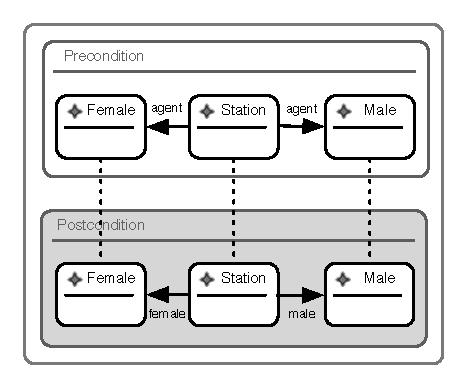
\includegraphics[width=1\textwidth]{./figures/policestation_dsltrans/satisfied.pdf}
%                \caption{Property 1 -- Expected to hold}
%                \label{fig:dsltrans_prop1}
%        \end{subfigure}%
%        ~~
%        \begin{subfigure}[b]{0.45\textwidth}
%                \centering
%                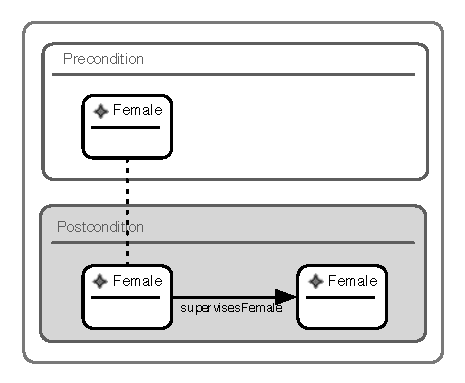
\includegraphics[width=1\textwidth]{./figures/policestation_dsltrans/unsatisfied.pdf}
%                \caption{Property 2 -- Not expected to hold}
%                \label{fig:dsltrans_prop2}
%        \end{subfigure}%
%        \caption{ Properties to be proved on the Police Station transformation}
%        \label{fig:properties}
%\end{figure}

\subsection{Satisfaction of a Property}
\label{sec:prop_satisfaction}

Let us now detail how a transformation execution is said to satisfy a property. Due to the common structure between properties and transformation executions, this satisfaction is based on whether the property can be isomorphically found in the transformation execution.

\begin{definition}{Satisfaction of a Property by an Execution of a Transformation\\}
\label{def:sat_prop_ex}

Let $tr\in \textsc{Transf}^{sr}_{tg}$ be a transformation. Let also $p = \langle V,E,st,\tau,\\Pre,Post\rangle \in \textsc{Property}(tr)$ be a property of $tr$ and $ex = \langle V',E',\\st',\tau',Input,Output\rangle \in Exec(tr)$ be an execution of $tr$. Execution $ex$ satisfies property $p$,  written $ex \models p$, if and only if:
\begin{multline*}
\forall f\; \exists g\,.\,\big(Pre \stackrel{f}{\vartriangleleft} Input^{*} \implies p \stackrel{g}{\vartriangleleft} ex^*\big)\\\text{where } V(Input)\cap CoDom(g) = CoDom(f)
\end{multline*}
% \begin{enumerate}
% \item $\langle V_p,E_p\setminus Il_p,\tau_p\rangle$ is a typed subgraph of $\langle V_x, E_x,\tau_x\rangle$
% \item if $v_p\rightarrow v_{p}'\in Il_p$ then there exists $v_x\rightarrow
% v_{x}'\in E_{x}^{*}$ where $\tau(v_p)=\tau(v_x)$, $\tau(v_p')=\tau(v_x')$ and
% $E_{x}^{*}$ is obtained by the transitive closure of $E_{x}$.
% \end{enumerate}
\end{definition}

\Cref{def:sat_prop_ex} states that, every time a graph that is isomorphic to the property's pre-condition is found in (the containment transitive closure of) the input model of the transformation's execution, a graph that is isomorphic to the complete property needs to be found in (the containment transitive closure of) the transformation execution. Note that the last part of the proposition in \cref{def:sat_prop_ex} ensures that the graph that is isomorphic to the property's pre-condition and the graph that is isomorphic to the complete property overlap on their pre-condition parts.

% resulting from the input pattern of $ex$ identified as pre-condition by $f$. Generally speaking, whenever the property's pre-condition is isomorphically found as a pattern of the input model of a execution, the property's post-condition must also be isomorphically found in the output generated from that input pattern. Note that, because a property may contain traceability links between the pre- and post-condition elements, it is necessary to check that those traceability links are also present in the execution. Because of this, the $g$ homomorphism in definition~\ref{def:sat_prop_ex} that checks the property's post-condition is such that it considers the same match pattern identified by the $f$ homomorphism when the pre-condition is checked.

\Cref{fig:prop_execution_without_traceability} demonstrates how a property holds on a transformation execution. Note that the lack of traceability links in the property means no element creation dependencies have been specified. In contrast, the traceability links in the property in \cref{fig:prop_execution_with_traceability} specify that the 'x:X' element must have been created from the 'b:B' element in the transformation execution. This is not the case (as highlighted by the dashed red circle), and therefore the property does not hold on the transformation execution.

\begin{figure}[htb]
        \centering
        \begin{subfigure}[b]{0.40\textwidth}
                \centering
                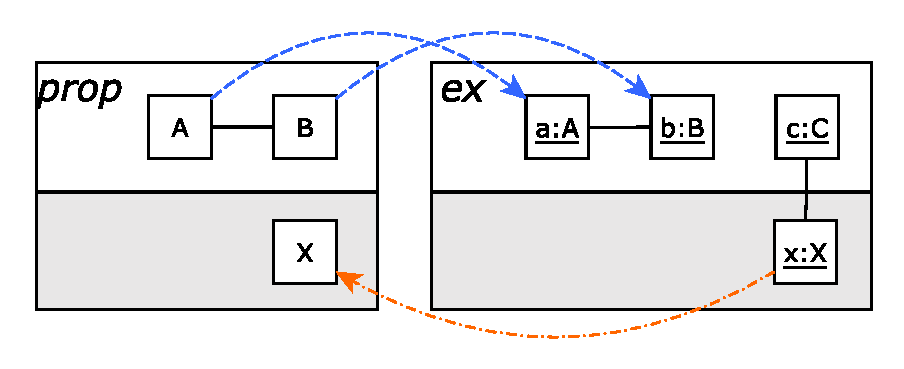
\includegraphics[width=1\textwidth]{./figures/property_proving/prop_execution_without_traceability.pdf}
                \caption{Property holds}
                \label{fig:prop_execution_without_traceability}
        \end{subfigure}%
        \\
        \begin{subfigure}[b]{0.40\textwidth}
                \centering
                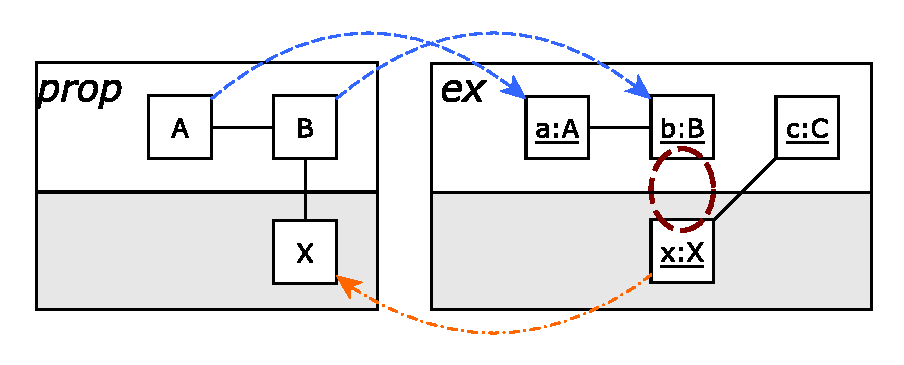
\includegraphics[width=1\textwidth]{./figures/property_proving/prop_execution_with_traceability.pdf}
                \caption{Property does not hold}
                \label{fig:prop_execution_with_traceability}
        \end{subfigure}%
        \caption{Matching property to a transformation execution}
        \label{fig:prop_execution}
\end{figure}

% \cref{def:sat_prop_pc} is similar to that of property satisfaction for a transformation execution, but for path conditions. Again, the property is isomorphically matched onto the respective graphs in the path condition.
% 
% Properties are proved on each path condition created by the path condition generation algorithm. Each path condition is examined to determine whether the pre-condition graph of the property can be isomorphically matched onto the match graph of the path condition, as in \cref{def:sat_prop_pc}. If this match cannot be performed, then the pre-condition does not hold for this path condition and this path condition will not be checked for this property.
% 
% If the pre-condition can be isomorphically matched to the match graph of the path condition, then we check if the entire
% property can be isomorphically matched to the path condition. Again, this is described in \cref{def:sat_prop_pc}. If this matching cannot be performed, then the property does not hold. The path condition itself then serves as a
% counter-example for the transformation property. The path condition also contains information on which rules were executed in the counter-example to permit further examination.
% 
% This property-checking can be done relatively quickly with efficient graph-matching techniques. \cref{sec:implementation} will briefly describe implementation and optimization details, while \cref{sec:experiments} presents two property-proving experiments.

Due to the fact an infinite amount of transformation executions exists, proving the property directly on the set of transformation executions is not possible. We thus rely on the finite set of path conditions to prove properties about the set of all transformation execution. Let us then define what it means for a property to hold on, or be satisfied by, a path condition.  

\begin{definition}{Satisfaction of a Property by a Path Condition\\}
\label{def:sat_prop_pc}

\reviewer{In Def. 31 I found it confusing that - different from previous
    definitions - the two morphisms now go in the same direction.
    There is an explanation after Definition 31, but I found it 
    very hard to understand.}
Let $tr\in \textsc{Transf}^{sr}_{tg}$ be a transformation. Let also $p = \langle V,E,st,\tau,\\Pre,Post\rangle \in \textsc{Property}(tr)$ be a property of $tr$ and $pc=\big\langle V',E',\\st',\tau', Match,Apply,Rulecop\big\rangle\in \textsc{Pathcond}(tr)$ be a path condition of $tr$. Path condition $pc$ satisfies property $p$, written $pc \vdash p$, if and only if:
\begin{multline*}
\forall f\; \exists g\,.\,\big(in\stackrel{f}{\blacktriangleleft} Pre \implies out \stackrel{g}\blacktriangleleft p\big)\\
\text{where } in \sqsubseteq Match^{*} \;\land\; out \sqsubseteq pc^{*}
\end{multline*}
Additionally $Dom(g)\cap Match(pc^{*}) = Dom(f)$ and $f(v)\neq f(v')$, $g(v)\neq g(v')$ whenever $v$ and $v'$ are elements of the path condition belonging to the same rule copy of set $Rulecop$.

\end{definition}

The principle behind the satisfaction relation in \cref{def:sat_prop_pc} is the same as the one behind the satisfaction relation between a property and an execution of a transformation in \cref{def:sat_prop_ex}: whenever the property's pre-condition is found in the path condition then so is the complete property. Also, those two graphs found in the path condition share the property's pre-condition part. This last condition enforces that the pre- and post-conditions of the property are correctly linked by symbolic traceability links in the path condition.

Note that, despite their semantic similarity, the relations are expressed differently in \cref{def:sat_prop_ex} and \cref{def:sat_prop_pc}. In \cref{def:sat_prop_ex} -- \emph{satisfaction of a property by an execution of a transformation}, typed graph injective homomorphisms are defined from the property into the execution. However, in \cref{def:sat_prop_pc} the direction of the typed graph surjective homomorphisms is from the path condition into the property. This can be explained by the fact, mentioned previously in this text, that different rules in a path condition may have elements that match over the same concrete instances of a transformation's input model. As such, we need to consider the case where match elements of a path condition, originating from different rules, overlap. 

\begin{figure}[htb]
 \centering
                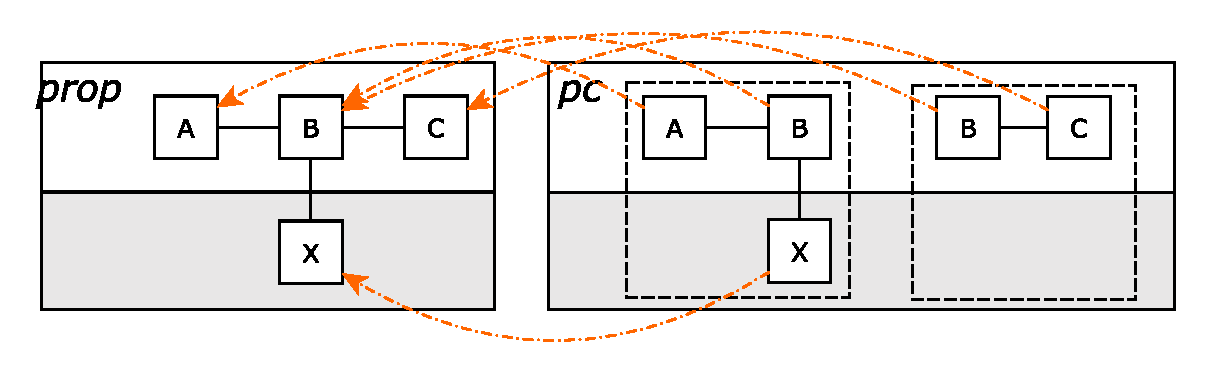
\includegraphics[width=0.44\textwidth]{./figures/property_proving/prop_pc.pdf}
                \caption{Property satisfied by a path condition}
                \label{fig:prop_pc}
\end{figure}

This overlapping is modeled by the surjective typed graph homomorphisms of \cref{def:sat_prop_pc} having the property as co-domain. The surjections allow ``forgetting'' that two match elements of the path condition belong to different rules. Note however that these surjections are special, as two elements belonging to the same copy of a rule have to be mapped injectively onto the property. This situation is depicted in \cref{fig:prop_pc}. Note that element $B$ is successfully matched even though it appears in two different rules in the path condition. 



\subsection{Expressiveness of the Property Language}
\label{subsec:expressiveness_prop}

As a result of taking rule combination (\cref{sec:building_pcs}) and overlap (\cref{sec:prop_satisfaction}) into consideration, our technique allows proving properties of transformation executions that are matched and built by multiple rules. This is the main goal of our work, as the properties we are interested in regard all possible interactions of rules in a DSLTrans transformation. However, an expressiveness limitation of the property language exists: we cannot prove properties having pre-conditions that can be found by executing the exact same rule more than once. This is natural, as by definition our abstraction only considers one exemplar of each rule per path condition having the exact same type for each match element. 

In order to illustrate this limitation, consider a transformation having one single rule that matches an element of type A and that produces an element of type X. Our technique will create a path condition as seen in \cref{fig:unprovable_pc}, abstracting over the number of times this rule has executed. According to the definition of satisfaction of a property by a path condition in \cref{def:sat_prop_pc}, the property in \cref{fig:unprovable_prop} does not hold on the path condition in \cref{fig:unprovable_pc}, although intuitively it should.

\begin{figure}[htb]
        \centering
        \begin{subfigure}[b]{0.144\textwidth}
                \centering
                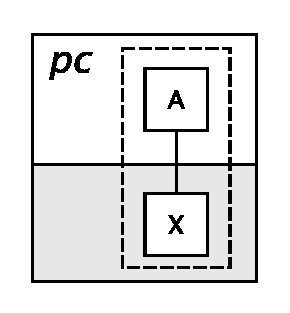
\includegraphics[width=1\textwidth]{./figures/property_proving/unprovable_rule.pdf}
                \caption{Path condition created from a rule}
                \label{fig:unprovable_pc}
        \end{subfigure}%
        ~~
        \begin{subfigure}[b]{0.20\textwidth}
                \centering
                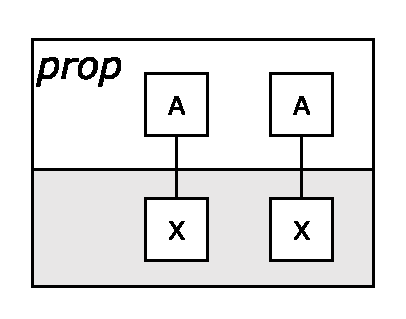
\includegraphics[width=1\textwidth]{./figures/property_proving/unprovable_prop.pdf}
                \caption{Property with multiple instances of rule elements}
                \label{fig:unprovable_prop}
        \end{subfigure}%
        \caption{Example of unprovable property}
        \label{fig:unprovable_property}
\end{figure}

Although this might be seen as a limitation of our technique, our case studies thus far indicate that very interesting properties exist that exclusively regard interactions between different rules. Nonetheless, our technique could be extended in order to consider more than one exemplar of the same rule per path condition. In fact, theoretically we already consider more than one exemplar of each rule when we treat polymorphism during path condition generation (see \cref{def:path_cond_gen}). However, in this case all expanded rules for a rule $rl$ are considered to be different as they differ by at least the type of one match element. Although this extension seems to fit relatively simply in our current theory, additional steps would need to be taken to understand which rules would be interesting to replicate to prove a particular property, and how many exemplars of each rule should be considered. In operational terms the number of replicas to consider of each rule is very important, given the exponential complexity of our path condition generation and property proof algorithms. Another possibility to tackle this issue would be to investigate and implement a more powerful satisfaction relation between path conditions and properties than the one we now present in \cref{def:sat_prop_pc}.
%Note however that the homomorphisms are injective when two elements belong to the same rule.\levi{explain this better}

% Given these definitions, we see that as all transformation executions are represented by path conditions, proving properties on the path conditions allows us to conclude property validity on all transformation executions.




\subsection{Validity and Completeness}
\label{subsec:prop_proving_valid_complete}

As for the path condition building algorithm, \emph{validity} and
\emph{completeness} need to be examined regarding our property verification
algorithm. In this context \emph{validity} means that if a property is satisfied by all path conditions generated for a transformation $tr$, then that property is satisfied by all executions of that transformation. On the other hand, if the property is not satisfied by at least one path condition, then it will not be satisfied by at least one transformation execution. In other words, we wish to show that no false positive or false negative proof results are induced by the abstraction relation.

% The proof of of these statements necessarily relies on the abstraction relation formally presented in\cref{def:instance_pc_ex}.

On the other hand, \emph{completeness} means that we are sure that all properties that can be expressed about a transformation can be shown to hold or not hold in all transformation executions.

As with the proofs for the validity and completeness of the abstraction relation, we present only proof sketches in this section in the interest of readability. Full proofs are shown in \cref{sec:val_complete_prop_verif} as \cref{prop:proof_validity_appendix} and \cref{prop:proof_completeness_appendix}.

% \subsubsection{Validity}
% 
% In this section we prove the validity of our property proof algorithm by considering what it
% formally means when a property is proved on a path condition. We argue that if
% the property holds or not on the path condition, then it will accordingly hold
% or not on for any transformation executions that the path condition represents.

% As well, we also prove that if a property holds or not on a specific transformation
% execution, it will hold or not on the path condition that represents that
% transformation execution.
\begin{proposition}{(Validity) The result of proving a property on a set of path conditions generated for a transformation or an all executions of that transformation is the same.\\}
\label{prop:proof_validity_appendix}
Let $tr\in \textsc{Transf}^{sr}_{tg}$ be a transformation and $p \in \textsc{Property}(tr)$ be a
property of $tr$. This given, we have that transformation $tr$ satisfies property $p$ if and only if:
\begin{equation}
\label{eq:prop_proof_transf_appendix}
\bigwedge_{pc\in \textsc{Pathcond}(tr)} pc\vdash p \hspace{.3cm} \Longleftrightarrow \hspace{.3cm} \bigwedge_{ex\in \textsc{Exec}(tr)}ex\models p
\end{equation}
\end{proposition}
\begin{pf}
In order to prove the proposition in \cref{eq:prop_proof_transf_appendix} we will start by demonstrating that,
if property $p$ holds on a path condition $pc$ generated for $tr$,
then $p$ will necessarily hold on any execution $ex$ of $tr$ that is abstracted by $pc$. On the other hand, if $p$ does not hold on $pc$ then it will not hold for at least of one execution $ex$ of $tr$ abstracted by $pc$. This lemma can be stated as follows:
\begin{equation}
\label{eq:prop_proof_pc_appendix}
pc\vdash p \;\Longleftrightarrow \;\forall ex\in\{ex\in\textsc{Exec}(tr)\;|\;ex\Vvdash pc\}\;.\; ex\models p
\end{equation}
We thus need to demonstrate both directions of the equivalence in \cref{eq:prop_proof_pc_appendix}. On the one hand we need to prove of the left-to-right direction of the equivalence:
\begin{multline}
\label{eq:prop_proof_left_right_appendix}
pc\vdash p \;\Longrightarrow \;\forall ex\in\{ex\in\textsc{Exec}(tr)\;|\;ex\Vvdash pc\}\;.\; ex\models p
\end{multline}
Proposition~\ref{eq:prop_proof_left_right_appendix} is shown to be true in \cref{lemma:validity1_appendix}.
We then need to show the right-to-left direction of the equivalence:
\begin{multline}
\label{eq:prop_proof_right_left_appendix}
\forall ex\in\{ex\in\textsc{Exec}(tr)\;|\;ex\Vvdash pc\}\;.\; ex\models p \;\Longrightarrow \;pc\vdash p 
\end{multline}
Proposition~\ref{eq:prop_proof_right_left_appendix} is shown to be true in \cref{lemma:validity2_appendix}.
Once propositions~\ref{eq:prop_proof_left_right_appendix} and~\ref{eq:prop_proof_right_left_appendix} are proved, we know that all path conditions on which a property holds represent executions on which the property also holds. Thus, if the property holds on all path conditions then it necessarily holds on all executions. On the other hand, if a property does not hold on one path condition, making it such that the conjunction on the left side of the equivalence in \cref{eq:prop_proof_transf_appendix} is false, then according to \cref{eq:prop_proof_pc_appendix} an execution for which it also does not hold exists. This makes it such that the conjunction on the right side of the equivalence in \cref{eq:prop_proof_pc_appendix} is also false.
\end{pf}

\begin{lemma}{If a property holds for a path condition then the property holds for any transformation execution that path condition abstracts.\\}
\label{lemma:validity1_appendix}
Let $tr$ be a transformation, $pc\in \textsc{Pathcond}(tr)$ be a path condition of $tr$, $ex\in \textsc{Exec}(tr)$ be an execution of $tr$ and $p\in \textsc{Prop}(tr)$ be a property of $tr$. Then we have that:
\begin{equation}
\label{prop:validity1_appendix}
pc\vdash p \;\Longrightarrow \;\forall ex\in\{ex\in\textsc{Exec}(tr)\;|\;ex\Vvdash pc\}\;.\; ex\models p
\end{equation}
\end{lemma}
\begin{pf}
By \cref{def:sat_prop_pc_appendix} we know that $pc\vdash p$ is equivalent to proposition $\forall f\; \exists g\,.\,\big(in\stackrel{f}{\blacktriangleleft} Pre \implies out \stackrel{g}\blacktriangleleft p\big)$, where $Pre$ is $p$'s pre-condition, $in$ is a subgraph of the containment transitive closure of the match part of $pc$, and $out$ is a subgraph of the containment transitive closure of $pc$. Additionally, by \cref{def:sat_prop_ex_appendix} we also know that $ex\models p$ is equivalent $\forall f\; \exists g\,.\,\big(Pre \stackrel{f}{\vartriangleleft} Input^{*} \implies p \stackrel{g}{\vartriangleleft} ex^*\big)$, where $Input$ is the input part of $ex$.

We will show that the implication holds by analysing the three cases where, $pc\vdash p$, the left side of Proposition~\ref{prop:validity1_appendix} holds.  
\begin{enumerate}
  \item If the precondition of the property cannot be found in the match part of a path condition $pc$, then it cannot be found in the input part of an execution abstracted by $pc$. Formally, we have that, assuming $ex$ is abstracted by $pc$:
\begin{equation}
\label{item:nopre}
\nexists f\,.\,\big(in\stackrel{f}{\blacktriangleleft} Pre\big) \implies \nexists f'\,.\, Pre \stackrel{f'}{\vartriangleleft} Input^{*}
\end{equation}
where, as before, $Input^{*}$ is the containment transitive closure of of the input part of $ex$ and $in$ is a subgraph of the match part of $pc$. Proposition~\ref{item:nopre} holds because of the fact that the surjection between $in$ and $Pre$ is defined such that it is in fact a set of injective typed graph homomorphisms between subgraphs of $in$ belonging to different rule copies that compose $pc$, and $Pre$. We know such a set of injective typed graph homomorphisms cannot be found from $in$ into $Pre$. However, the abstraction relation in \cref{def:abstraction_pc_ex_appendix} states that an injective typed graph homomorphism exists between each rule copy in the match part of $pc$ and $Input^{*}$. We thus know that there cannot exist an injective typed graph homomorphism between $Pre$ and $Input^{*}$. 
  \item For certain executions, the property holds on the path condition but the property's pre-condition cannot be found in the execution.
\begin{equation}
\label{item:prepostnotholds}
\forall f\; \exists g\,.\,\big(in\stackrel{f}{\blacktriangleleft} Pre \land out \stackrel{g}\blacktriangleleft p\big) \implies \nexists f'\,.\,\big(Pre \stackrel{f'}{\vartriangleleft} Input^{*}\big)
\end{equation}
These are the executions where a set of injective typed graph homomorphisms can be found from $in$ into $Pre$, but not from $in$ into $Input^{*}$, as required by the abstraction relation. If this is the case then this means that at least two vertices of $in$ belonging to different rule copies that were mapped by $f$ into the same vertex of $Pre$, are mapped into different vertices of $Input^{*}$ by $f'$ (or vice-versa). 
  \item For the remaining set executions abstracted by $pc$, if the property holds on the path condition then the property holds on the execution. Formally, according to \cref{def:sat_prop_pc_appendix} and \cref{def:sat_prop_ex_appendix} we have that:
\begin{multline}
\label{item:prepostholds}
\forall f\; \exists g\,.\,\big(in\stackrel{f}{\blacktriangleleft} Pre \land out \stackrel{g}\blacktriangleleft p\big) \implies \\\forall f'\; \exists g'\,.\,\big(Pre \stackrel{f'}{\vartriangleleft} Input^{*} \land p \stackrel{g'}{\vartriangleleft} ex^*\big)\\
\text{where } Dom(g)\cap Match(pc^{*}) = Dom(f) \text{ and}\\
V(Input)\cap CoDom(g') = CoDom(f')
\end{multline}
This is the case where every two vertices of $in$ belonging to different rule copies that were mapped by $f$ into a common vertex of $Pre$, are also mapped into a common vertex of $Input^{*}$ by $f'$. We thus need to show that the fact that the post-condition of the property holds on the path condition implies that the post-condition of the property also holds on the execution, i.e. that $out \stackrel{g}\blacktriangleleft p \implies p \stackrel{g'}{\vartriangleleft} ex^*$. This proposition is true because we know by \cref{def:abstraction_pc_ex_appendix} of abstraction relation that a surjective typed graph homomorphism exists between the output part of $ex$ and the apply part of $pc$. By composing this surjection with the surjection between $out$ and $p$ we take as hypothesis, we know a surjective typed graph homomorphism exists between the output of $ex$ and $p$. The inverse of this composed homomorphism contains an injective typed graph homomorphism between $p$'s post-condition and $ex$. We are thus missing accounting for the traceability links between the pre- and post-condition of property $p$, if they exist.  According to Proposition~\ref{item:prepostholds} we know that $in$ and $out$ overlap on their subgraphs that are isomorphic to $p$'s precondition. By \cref{def:abstraction_pc_ex_appendix} of the abstraction relation, we know that an injective typed graph homomorphism can be found between each strongly connected component formed of symbolic traceability links of $pc$, and $ex$. We also know that a typed graph surjective homomorphism exists between $out$ and $p$. We thus know that the traceability links between the pre- and post-condition of $p$ can be injectively found in $ex$. Note that strongly disjoint connected symbolic traceability link components mapped from $pc$ to $ex$ may be mapped onto joined traceability link components in $ex$ when disjoint vertices of the match part of $pc$ are mapped onto the same input vertex in $ex$. 
\end{enumerate}

The three cases above cover all executions that can be abstracted by a path condition, and as such we know that if the property holds on a path condition, it will necessarily hold on all the executions that path condition abstracts.
\end{pf}
% 
\begin{lemma}{If a property holds for a transformation execution then the property holds for the path condition that abstracts it.\\}
\label{lemma:validity2_appendix}
Let $tr$ be a transformation, $pc\in \textsc{Pathcond}(tr)$ be a path condition of $tr$, $ex\in \textsc{Exec}(tr)$ be an execution of $tr$ and $p\in \textsc{Prop}(tr)$ be a property of $tr$. Then we have that:
\begin{equation}
\label{eq:prop_proof_right_left_appendix2}
\forall ex\in\{ex\in\textsc{Exec}(tr)\;|\;ex\Vvdash pc\}\;.\; ex\models p\;\Longrightarrow \; pc\vdash p
\end{equation}
\end{lemma}
\begin{pf}
We will demonstrate Proposition~\ref{eq:prop_proof_right_left_appendix2} holds by contraposing it:
% By using contraposition we can show that:
\begin{multline}
\label{eq:prop_proof_right_left_contra}
\neg(pc\vdash p) \;\Longrightarrow \;\\\exists ex\in\{ex\in\textsc{Exec}(tr)\;|\;ex\Vvdash pc\}\;.\; \neg(ex\models p)
\end{multline}

By \cref{def:sat_prop_pc_appendix} we know that $pc\vdash p$ is equivalent to proposition $\forall f\; \exists g\,.\,\big(in\stackrel{f}{\blacktriangleleft} Pre \implies out \stackrel{g}\blacktriangleleft p\big)$, where $Pre$ is $p$'s pre-condition, $in$ is a subgraph of the containment transitive closure of the match part of $pc$, and $out$ is a subgraph of the containment transitive closure of $pc$. We also know by \cref{def:sat_prop_ex_appendix} that $ex\models p$ is equivalent $\forall f\; \exists g\,.\,\big(Pre \stackrel{f}{\vartriangleleft} Input^{*} \implies p \stackrel{g}{\vartriangleleft} ex^*\big)$, where $Input$ is the input part of $ex$. After replacing the left and the right hand side of Proposition~\ref{eq:prop_proof_right_left_contra} by equivalent formulas and solving the negations we reach the conclusion we need to prove:
\begin{multline}
\label{eq:prop_proof_right_left_contra_neg}
\exists f\; \forall g\,.\,\big(in\stackrel{f}{\blacktriangleleft} Pre \land \neg(out \stackrel{g}\blacktriangleleft p)\big) \;\Longrightarrow \;\\\exists ex\in\{ex\in\textsc{Exec}(tr)\;|\;ex\Vvdash pc\}\;.\;\\ \exists f'\; \forall g'\,.\,\big(Pre \stackrel{f'}{\vartriangleleft} Input^{*} \implies \neg(p \stackrel{g'}{\vartriangleleft} ex^*)\big)
\end{multline}

We thus need to demonstrate that whenever the pre-condition of the property is found at least once in a path condition, but not its corresponding post-condition, then the same thing happens for at least one of the executions abstracted by that path condition. We know by Proposition~\ref{eq:prop_proof_right_left_contra_neg} that $in\stackrel{f}{\blacktriangleleft} Pre$, i.e. the precondition of the property is found at least once in the path condition. We thus know that there exists one execution for which $Pre \stackrel{f'}{\vartriangleleft} Input^{*}$ holds, which is the execution for which the surjective typed graph homomorphism $f$ maps vertices belonging to the match parts of different rule copies in the same fashion that the set of injective typed graph homomorphisms from the abstraction relation in \cref{def:abstraction_pc_ex_appendix} maps to the match part of $pc$ onto $input^{*}$.

In order to complete the proof we need to show that the fact that $\neg(out \stackrel{g}\blacktriangleleft p)$, i.e. if the complete property cannot be found in the path condition, then $\neg(p \stackrel{g'}{\vartriangleleft} ex^*)$, i.e. the complete property cannot be found in the execution. Note that, according to \cref{def:sat_prop_pc_appendix} and \cref{def:sat_prop_ex_appendix}, we know the considered complete property graphs both in $p$ and $ex$ found by $g$ and $g'$ are anchored on the pre-condition graphs of the property found by $f$ and $f'$. Because of the abstraction relation, we know a surjective typed graph homomorphism between the output of $ex^{*}$ and the apply part of $pc$ exists. Given a surjective typed graph homomorphism does not exist between $pc$ and $p$, we know certain vertices and/or edges that exist in $p$, either in its apply part or in its symbolic traceability links, do not exist in $pc$. If the missing vertices and/or edges are part of the $apply$ part of $p$ then we are sure an injective typed graph homomorphism cannot exist between $p$ and $ex$ because $ex$ also does not contain those vertices or edges. If the missing edges are symbolic traceability edges then, according to the condition on strongly connected components in the abstraction relation in \cref{def:abstraction_pc_ex_appendix}, we know that the traceability links in $ex$ can be surjectively mapped onto $pc$. Because some of those traceability links are missing in $p$, an injective typed graph homomorphism cannot exist between $p$ and $ex$. 


% We only need to worry about the case where we have  $ex\Vvdash pc\land
% \neg(pc\vdash p)$ given our property proof results are meaningful only for
% transformation executions which are abstracted by the path condition being
% examined\levi{because by the unicity result one execution is only abstracted by one path condition}. In this
% case we have that, because $ex\Vvdash pc$, by \cref{def:abstraction_pc_ex} we know
% that there is a surjective typed graph homomorphism between between the apply
% pattern of transformation execution $ex$ and the apply pattern of the path
% condition $pc$. Given we know that $\neg(pc\vdash p)$, then we know that an
% injective type graph homomorphism does not exist between $p$ and $pc$. This
% means that, by the \cref{def:typed_graph_homomorphism} of injective typed graph
% homomorphism, there exists a type $T$ which is instantiated in $pc$ but not in
% $prop$. However, because of the fact that $ex\Vvdash pc$ we know that $T$ is
% instantiated in $ex$ because a surjective typed graph homomorphism exists
% between $ex$ and $pc$, implying type $T$ is instantiated at least once in $ex$.
% We thus can deduce that we have $\neg(ex\models p)$ given that $ex\models p$
% implies that there exists an injective type graph homomorphism between property
% $p$ and execution $ex$. This injective type graph homomorphism cannot exist
% given the fact an instance of $T$ exists in $ex$ but not in $p$.

\end{pf}


\begin{proposition}{(Completeness) Properties of a transformation can be shown to either hold for all transformation executions, or not hold for at least one transformation execution.}
\label{prop:proof_completeness}
\end{proposition}
\begin{pf}
This result follows from two previous results: \cref{prop:pc_completeness}, that tells us that every transformation execution is abstracted by one path condition; and \cref{prop:proof_validity} that shows us that every path condition is taken into consideration during property proof. Note that \cref{lem:uniqueness} guarantees consistency of our results, in the sense that the uniqueness of one path condition per transformation execution guarantees that a property cannot be proven to be both \emph{true} and \emph{false} for two path conditions representing the same transformation execution.
\end{pf}


\section{Implementation Details}
\label{sec:implementation}

In this section we will briefly describe our implementation of the algorithms described in the above sections. In particular, we highlight optimizations made and provide results suggesting that our algorithms can feasibly scale to industrial-sized applications.

\subsection{Enabling Technology and Prototype}

In previous work we have reported on the usage of Prolog as a means to build a
proof-of-concept prototype for our technique~\cite{Lucio:10}. The experiments
performed using Prolog were inconclusive regarding the scalability of our
technique given that the path condition construction algorithm as now described in \cref{sec:building_pcs} lacked a formal understanding, as well as several other
imprecisions. As such, no performance optimisations were attempted.

Through our sponsorship by the NECSIS (Network for the Engineering of Complex
Software-Intensive Systems for Automotive Systems) project, we have the
opportunity to apply our verification technique in an industrial setting. In
order to achieve high performance in this setting, despite the complexities of
verification techniques, we were required to choose an underlying efficient
implementation framework. Our goals were to select a framework which: 1) allows
graph manipulation natively. This detaches us from the worries of building and
optimising our own subgraph isomorphism NP-complete algorithms, which are
constantly used during path condition construction; and 2) allows detailed control over
graph manipulation such that the implementation of complex optimizations is feasible. These optimizations are potentially required to apply our technique to large and complex model transformations.

We have chosen T-Core~\cite{DBLP:journals/eceasst/SyrianiV10,SyrianiVanghel:13}
as our graph manipulation framework.
Aside from satisfying our basic requirements described above, T-Core allows
for native rewriting of typed graphs, which considerably eases our implementation
effort. The algorithms described throughout this work have been implemented by scheduling T-Core
graph manipulation primitives using the Python programming language. 

\subsection{Complexity}
\label{sec:complexity}

Let us motivate our discussions of optimisation and performance by providing an
approximate formula for the complexity of the path condition construction and
property proof algorithms presented in Sections~\ref{sec:building_pcs}
and~\ref{sec:verif_dsltrans_props}.

\subsubsection{Path Condition Generation}
Recall that a DSLTrans transformation is composed of rules arranged in layers.
The path condition generation algorithm described in \cref{sec:building_pcs}
moves through these layers and combines rules into viable path conditions.

Let the number of rules in the transformation be $r$.  Then, the maximum number
of path conditions that can be created is $2^{r}$. Each path condition will
either represent a rule or not, and therefore the $2^{r}$ path conditions
represent all possible rule combinations. Note that this case assumes that all
path conditions are viable. In practice, unsatisfied rule dependencies will
prevent some rule combinations, reducing the number of path conditions created.

As discussed in \cref{sec:building_pcs}, the path condition generation algorithm builds these path conditions by
considering all possibilities of how a rule can combine with a path condition. This
combination step is composed of two algorithmic components. The first is to
determine all positions where the rule matches over the path condition. Let this
matching step be $m$. Note that this matching step is dependent on the size of the rules.

The second step of the combination step is to "glue" the rule at all matching
positions. Let this step be termed $g$. This step is linear in the size of the rule to be glued multiplied by the number of times the rule has matched in step $m$.

Note that $m$ and $g$ could be quite expensive operations. However, in
our implementation, these steps are implemented using the efficient T-Core graph
manipulation framework.

\begin{equation}
\label{eq:complexity}
\mathcal{O}\big({2^r \cdot (m + g)}\big)
\end{equation}

\cref{eq:complexity} presents the time and space complexity for the path condition generation algorithm.

\subsubsection{Property Proof}
\label{subsubsec:complex_prop_proof}
For our property proving algorithm, recall that each path condition created is examined to see if the property in question holds.

As mentioned in \cref{sec:verif_dsltrans_props}, a path condition must be \\matched by the property. However, different elements in the path condition may overlap (have been matched on) on the same elements in the input model, as described in \cref{sec:prop_satisfaction}.
Therefore, an operational step is required to resolve this ambiguity. One solution is to produce all possible path conditions, where for each pair of overlapping elements in a path condition, one new path condition is produced where they are merged, and one new path condition where they are not.

The complexity of this ``disambiguation step'' will be proportional to the average number of overlapping elements in the path condition, and will be denoted by the term $d$ in this discussion. Practically, $d$ will be dependent on how rules are combined during the path condition generation algorithm. Future work will precisely detail how the characteristics of the transformation affect the algorithm's complexity.

The complexity of the matching step will then be linear in the size of the set of path conditions. The property matching step itself ($p$) will then be linear in the size of the property and path conditions. Again, in practice $p$ is implemented using the T-Core framework.

\begin{equation}
\label{eq:complexity2}
\mathcal{O}\big({2^r \cdot 2^d \cdot p}\big)
\end{equation}

\cref{eq:complexity2} shows time and space complexity for the property proving step.

\subsection{Optimisations}
\label{sec:optimization}

In order to tackle the time and space complexities of the path condition
construction and property proof algorithms we have employed several engineering 
strategies. In the following paragraphs we describe the most relevant of these
strategies.

\begin{itemize}
\item Path condition construction and property proof are very repetitive
processes since most individual rules are often composed and searched in 
the same manner. Since many similar situations have to be investigated during
path condition construction and property proof, memoisation was used whenever
possible to avoid isomorphic graph matching and rewrite operations.
As such caching is heavily used in both algorithms;

\item In \cref{subsubsec:complex_prop_proof} we detail how the overlap of elements in a path condition can be operationally handled by producing two new path conditions for each pair of overlapping elements. Given this procedure is recursive and presents exponential
time complexity, we have performed this ``disambiguation'' step only when strictly necessary:  when performing
property verification on a path condition that contains the elements in
the property.
Note that the fact that  disambiguation is performed in this lazy fashion
allows us to operationally keep path conditions as sets of individual rules.
This makes it possible to heavily reuse pointers to the original transformation
rules when building path conditions, thus reducing the algorithm's space complexity when compared to the explicit representation of
each generated path condition. This also means that, practically,
path condition disambiguation is mostly done on demand during property proving;

\item For property proof we have implemented a strategy to avoid checking path
conditions where the property is sure to hold. The strategy is based on the fact
that if a path condition $B$ contains the same elements as a path condition
$A$ where the property has already been checked successfully, and no additional
elements of the property exist in $B$, then the property also holds
for $B$.
\end{itemize}



\section{Experiments}
\label{sec:experiments}

This section will detail the experiments we performed in order to measure the performance of our technique. We present timing results for two experiments. The first is to obtain timing results for proving two properties on a synthetic transformation, while the second experiment is sourced from our industrial partners.

\subsection{Experimental Setup and Results}

The complexity of \cref{eq:complexity} and \cref{eq:complexity2} suggest that our property proving
approach is intractable in the general case. However, we have provided in \cref{sec:optimization} a number
of concrete optimisations to allow us to prove properties on transformations of
non-trivial size. This section will detail our experiments to determine the
effect of the number of rules in the transformation on the performance of our
implementation.

For our experiment we have used the Police Station transformation as described
in \cref{sec:dsltrans} as a sample transformation. However, in order to
determine the performance characteristics of our approach, we have replicated
the rules within the transformation.

This was achieved by synthetically augmenting the original metamodels by
replicating their elements twice, thus building source and
target metamodels that are three times larger. For example, in the source
metamodel we will now have \emph{Station1} (renamed from the original
\emph{Station} class) and its replicas \emph{Station2} and \emph{Station3}.
These three metamodel elements are distinct from each other and are formally
three different types. We have also added new rules that utilise these new
types, as seen in \cref{fig:replicated_police_station_trafo}.

\begin{figure}[bht] \centering 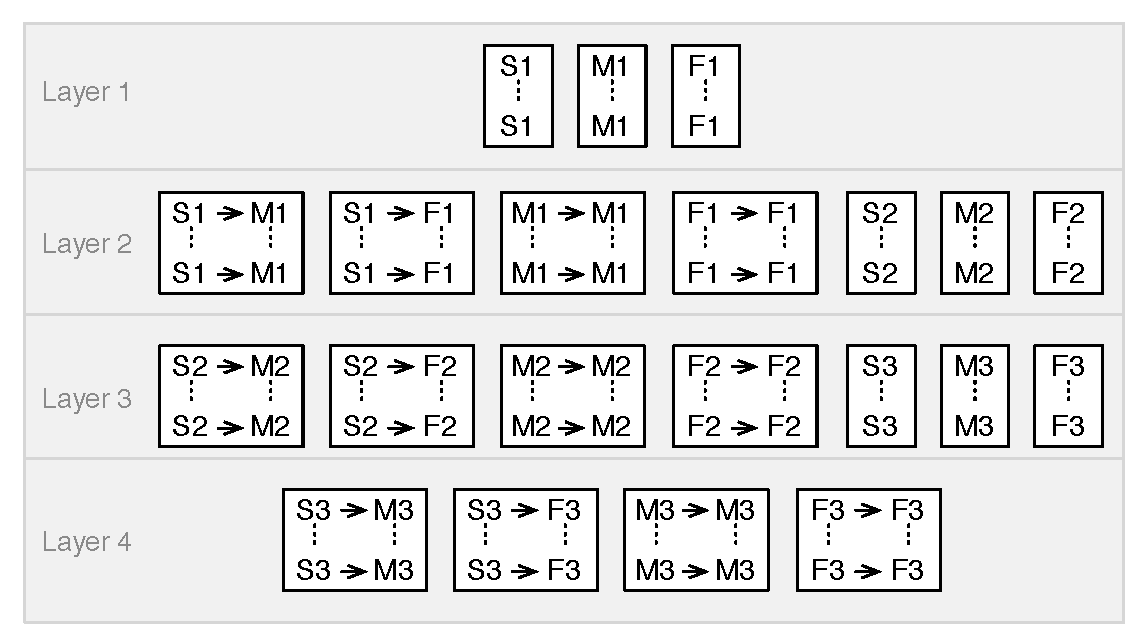
\includegraphics[width=0.48\textwidth]{./figures/policestation_dsltrans/3runtransformation.pdf}
	\caption{Replicated Police Station transformation for performance tests}
	\label{fig:replicated_police_station_trafo}
\end{figure}

Note that for clarity reasons in
\cref{fig:replicated_police_station_trafo} we have abbreviated the element
names \emph{Station}, \emph{Male} and \emph{Female} to \emph{S}, \emph{M} and
\emph{F} respectively. Additionally, the numerical suffix denotes which
replicated metamodel element is represented, as described above.



\renewcommand{\baselinestretch}{1.0}

\subsubsection{Results}

\begin{table*}[htb]
\label{table:results}
\centering
\begin{tabular}{|c|r|r|r|r|r|}
\hline
\rowcolor{Gray}
\parbox[t]{0.04\textwidth}{\# of rules\\} & 
\parbox[t]{0.13\textwidth}{\# of path conds. created\\} 
& \parbox[t]{0.15\textwidth}{Path conds. build time (s)\\}
& \parbox[t]{0.11\textwidth}{Memory used (KB)\\}  
& \parbox[t]{0.18\textwidth}{Proof time for property that holds (s)\\} 
& \parbox[t]{0.20\textwidth}{Proof time for property that does not hold (s)\\}\\
\hline
3	&	8		&	$<$0.01		&	0.08	&	-		&	-		\\
5	&	16		&	0.13		&	0.09	&	0.19		&	0.003	\\
7	&	34		&	0.39		&	0.17	&	1.26		&	0.003	\\
10	&	272		&	1.87		&	1.24	&	2.40		&	0.003	\\
12	&	442		&	2.68		&	1.83	&	3.40		&	0.003	\\
14	&	1156	&	9.00		&	4.98	&	8.38		&	0.003	\\
17	&	9248	&	59.08		&	38.01	&	73.51	&	0.003	\\
19	&	15028	&	97.52		&	60.10	&	140.77	&	0.003	\\
21	&	39304	&	369.19		&	156.79	&	412.02	&	0.003	\\
\hline
\end{tabular}
\caption{Results for creating the set of all path conditions and proving two properties}
\label{tab:scalability_results}
\end{table*}

\reviewer{Table 1, even if it was not experimented to exceed 0.003 seconds when proving for property that does not hold, maybe it would be possible to estimate the maximum time based on that measurement and the complexity formula.}

The results in \cref{tab:scalability_results} were obtained by verifying
the properties in Figures~\ref{fig:dsltrans_prop1}
and~\ref{fig:dsltrans_prop2} on the transformation seen in
\cref{fig:replicated_police_station_trafo}. The experimental platform was
a 2.2 GHz Intel Core i7 machine with 8GB of DDR3 memory running Ubuntu 11.10 and
Python 2.7. For each measurement involving time, we repeated the given
experiment three times and calculated the final result as the average of the
three experiment results. The code used to run our experiments can be found
at~\cite{DSLTransVerif:13}.




\subsubsection{Time Required to Produce Path Conditions}

An important metric for our work is measuring how long it takes to produce the final set of path conditions from a DSLTrans transformation. As seen in \cref{sec:complexity}, this metric depends on the composition of the rules in the transformation's layers.

The first column of \cref{tab:scalability_results} shows the number of
rules for each part of the experiment. In order to provide greater granularity in the data, and determine the precise effect of adding more rules to a layer versus adding another layer of rules, we examine subsets of rules taken from \cref{fig:replicated_police_station_trafo}. For example, the subset with five rules contains the three first rules of layer 1 plus the two first rules of layer 2; the subset with seven rules contains the first three rules of layer 1 plus the four first rules of layer 2; and so on.

\begin{figure*}[htb]
        \centering
        \begin{subfigure}[b]{0.26\textwidth}
                \centering
                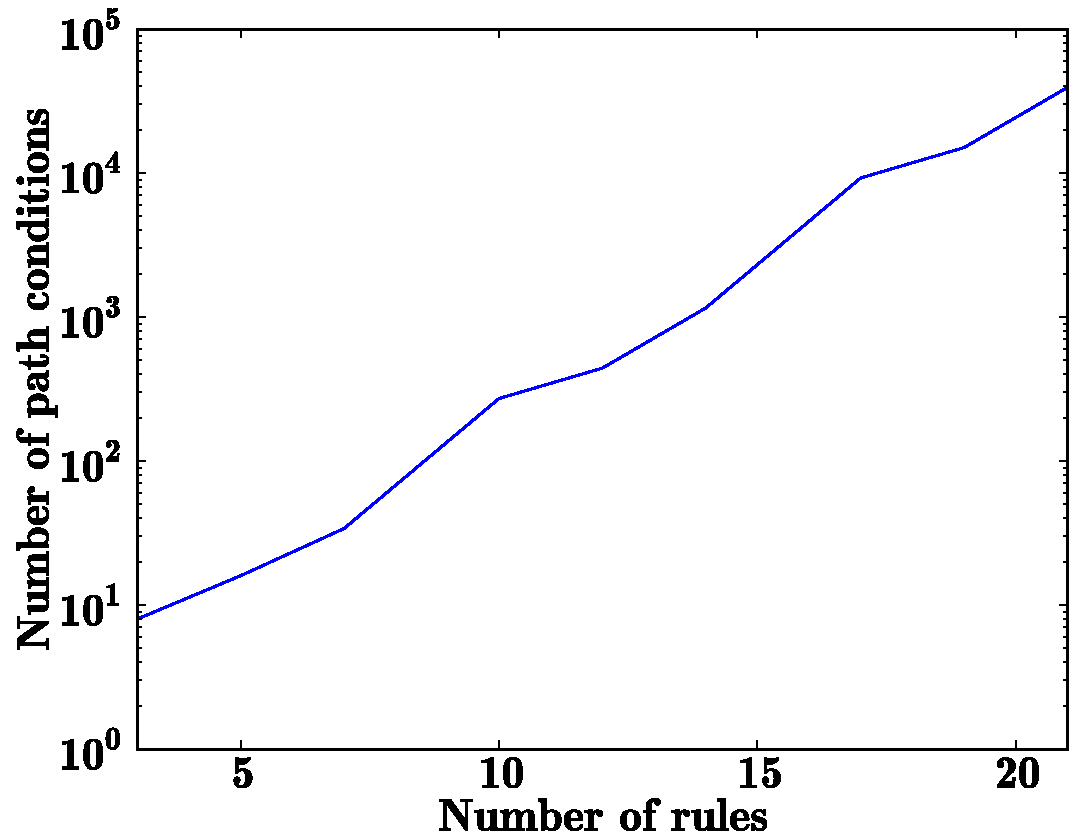
\includegraphics[width=1\textwidth]{./figures/results/rules_vs_pcs.pdf}
                \caption{Number of rules vs. \\path conds. created}
                \label{fig:rules_vs_pcs}
        \end{subfigure}%
        ~~
        \begin{subfigure}[b]{0.26\textwidth}
                \centering
                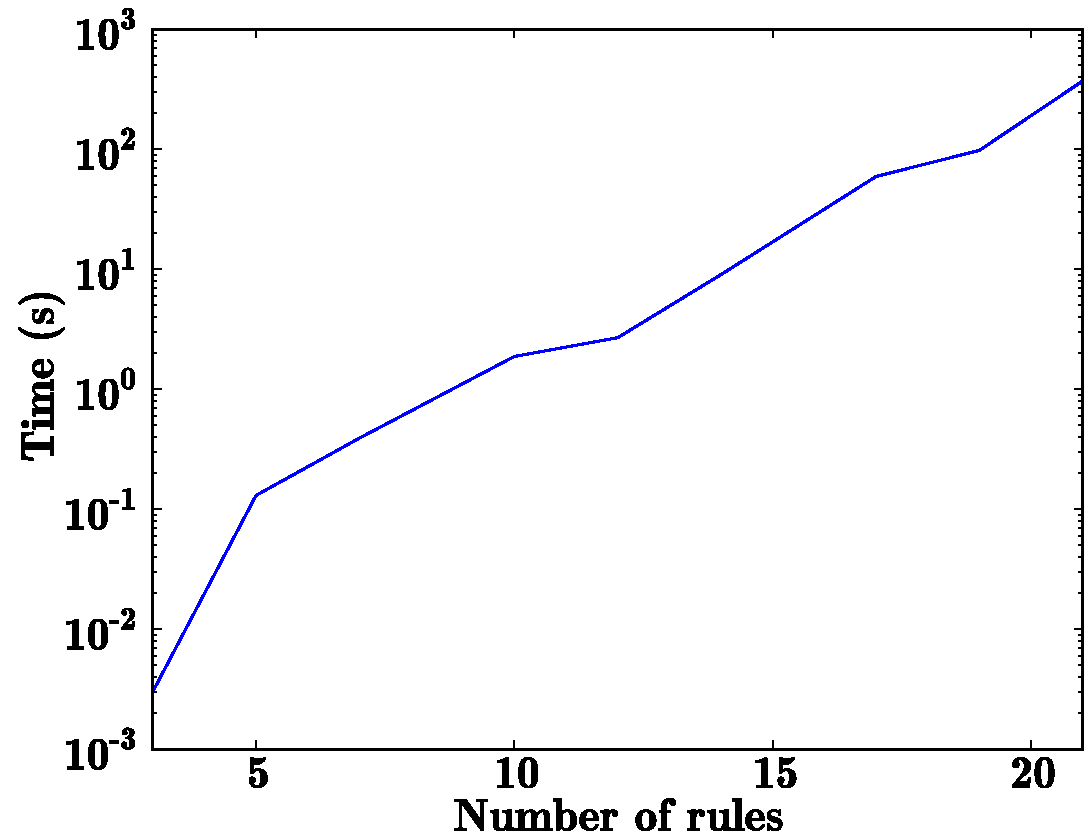
\includegraphics[width=1\textwidth]{./figures/results/rules_vs_time.pdf}
                \caption{Number of rules vs. \\time taken}
                \label{fig:rules_vs_time}
        \end{subfigure}%
        ~~
        \begin{subfigure}[b]{0.26\textwidth}
                \centering
                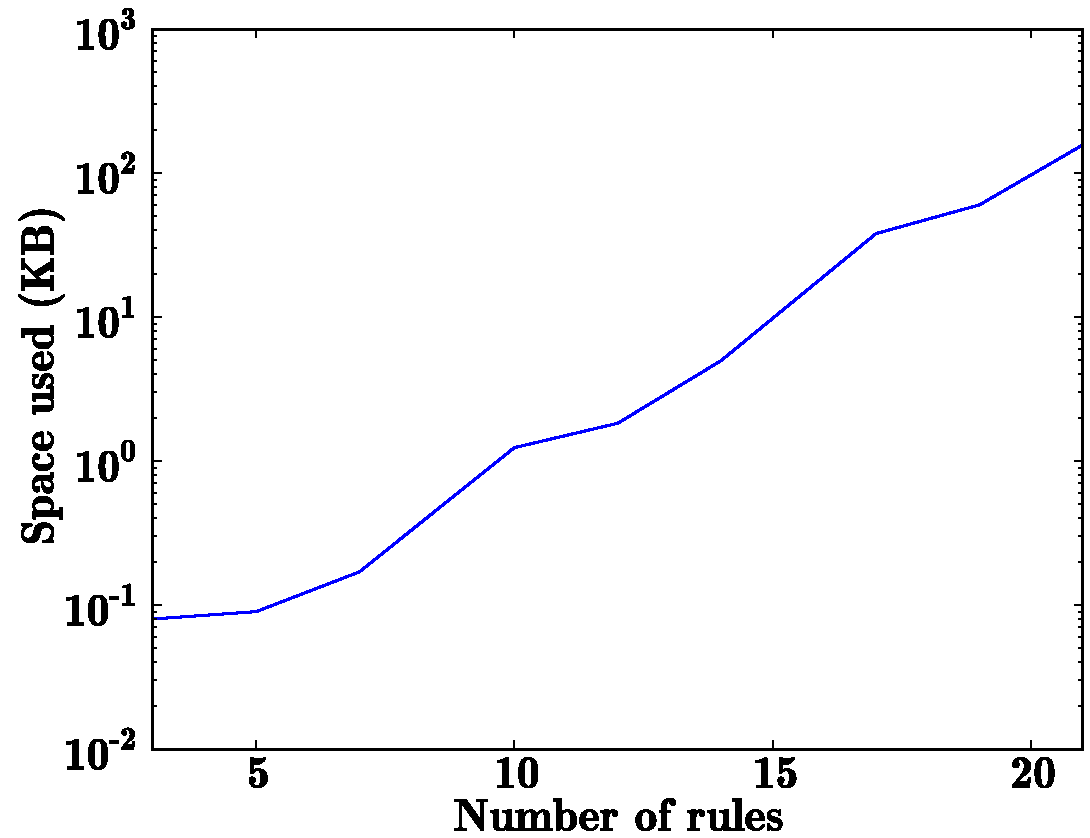
\includegraphics[width=1\textwidth]{./figures/results/rules_vs_memory.pdf}
                \caption{Number of rules vs. \\memory used}
                \label{fig:rules_vs_memory}
        \end{subfigure}%

        \caption{Metrics for the path condition creation process}
        \label{fig:path_condition_building}
\end{figure*}



\cref{fig:rules_vs_pcs} presents the number of path conditions created for
a given number of rules, while \cref{fig:rules_vs_time} graphs the time
taken to create all the path conditions. Both the number of path conditions and
the time required to build them rise steeply with the number of rules, but it
is quite feasible to build path conditions and prove properties for up to 21
rules. As shown later in the section on industrial experimentation, 21 rules
exceeds the number of rules in our industrial case study. It also exceeds the
number of rules in several useful DSLTrans
transformations~\cite{febavava:10,dsltrans_manual,zhang:ACP_APN:11}.

\cref{tab:scalability_results} and \cref{fig:rules_vs_memory} demonstrate that memory consumption is very modest, remaining well under a megabyte for thousands of path conditions. This is due to the optimisations that we perform, such as only storing pointers to path conditions. We are encouraged that this algorithm can scale extremely well in terms of respecting memory constraints.


\subsubsection{Time Required to Prove Properties}

We now examine the time it takes to prove two properties on the transformation based on the number of path conditions created from that transformation. The two properties to be proven are shown in \cref{fig:properties} in \cref{sec:dsltrans}. The first, in \cref{fig:dsltrans_prop1}, is a property that we expect to hold for all path conditions. \cref{fig:dsltrans_prop2} shows a property that we expect to \emph{not} hold for all path conditions. 

\begin{figure}[bht] \centering 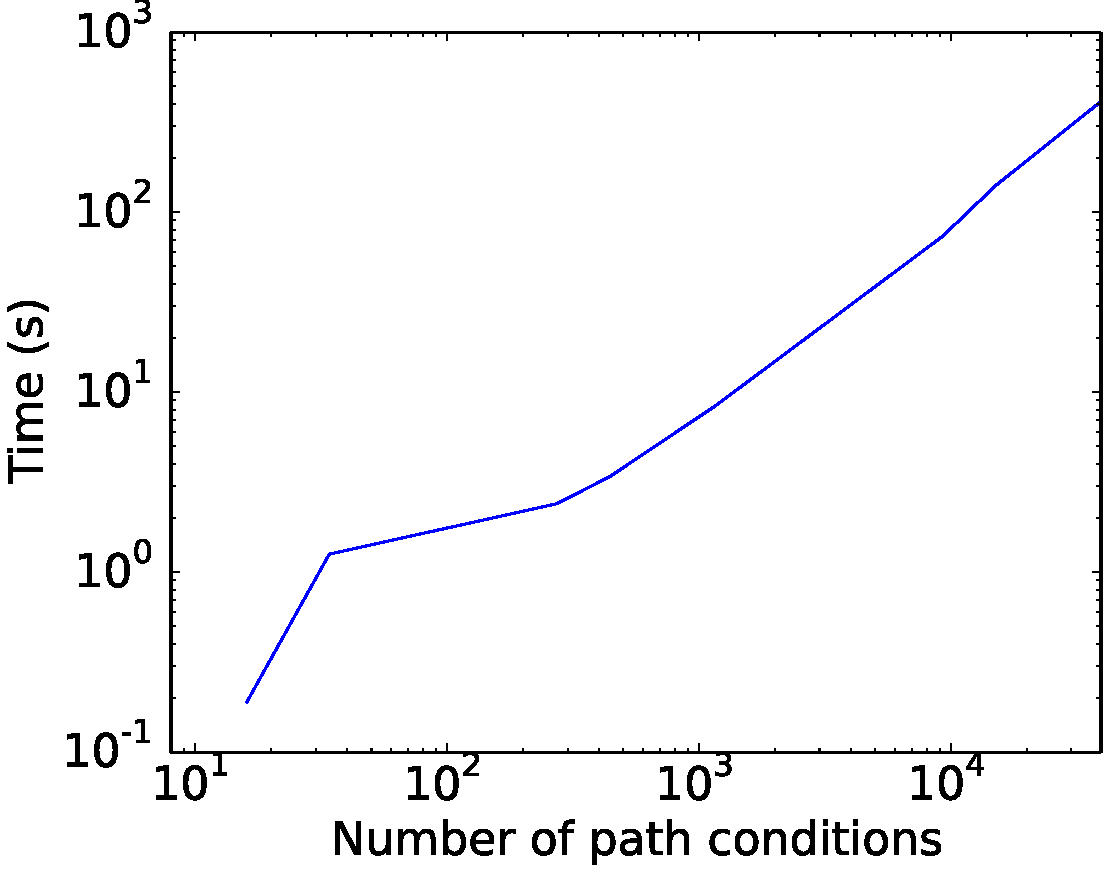
\includegraphics[width=0.35\textwidth]{./figures/results/pcs_vs_prop1.pdf}
	\caption{Time required to prove the property that holds on all path conditions}
	\label{fig:pcs_vs_prop1}
\end{figure}

\cref{fig:pcs_vs_prop1} shows the time in seconds required to prove the property that holds on all path conditions, as seen in the fifth column in \cref{tab:scalability_results}. Note that the time taken increases linearly with the number of path conditions to examine. This increase occurs as each property must be checked to ensure that the property will hold.

In contrast, the time required to disprove the property that does not hold is roughly constant. This can be seen in the sixth column in \cref{tab:scalability_results}, where this proof took 0.003 seconds regardless of the number of path conditions examined. This is due to the fact that, given the property does not hold, the proof algorithm can stop as soon as a counterexample is found. The very short time to disprove the property is due to the fact that path conditions are checked for the property sequentially, in the order they are produced. In our example, a counterexample can be found very early in the set of path conditions. Note that a more complex property that involves rules which would appear only much later in the generated set of path conditions would require a longer time to reach a counter-example.

Experiments were also undertaken to determine what effects the size of the property to be proved has on the running time of the algorithm. Preliminary results indicate that an increase of the property size results in a proportional increase in running time. This is to be expected, as the underlying graph matching algorithm has to match more elements to determine if the property holds or not.

% \levi{Do you want to keep this?}
% Finally, one last observation on the values in
% table~\ref{tab:scalability_results} is the fact that when rules without backward
% links are added to the transformation (the jumps from~7 to~10,~14 to~17 and~21
% to~24 rules) both the number of produced path conditions and the used memory
% increases around tenfold. Comparatively, when rules with backward links are
% added to the transformation (the jumps from ~3 to~7,~10 to~14 and 17 to~21
% rules) both the number of path conditions and the used memory only increases
% around five times. This is despite the fact that we increase rules with backward
% links by sets of 4 rules, whereas we increase rules without backward links by
% sets of 3 rules. The reason for this difference is the fact that, during
% symbolic execution construction, a rule with backward links may simply not be
% executable for a given path condition or can be merged with a previous path
% conditions. In both these cases no new path conditions are added to the symbolic
% execution. However, a rule without backward links necessarily generates twice
% the path conditions already generated by the symbolic execution algorithm as it
% may always be executed.
% 
% \levi{talk about better time optimizations here}It is however the case that, if
% no or few collapse operations are required for a path condition, the algorithm
% still attempts to collapse rules in this fashion. This may result in overhead as
% compared to merging all the rules and recursively collapsing. 

\subsection{Industrial Experimentation}
\label{sec:industrial_exp}

Aside from the experiments with the police station transformation we have
reported in the previous section, we have applied our technique in the context
of the NECSIS project.
The experiment regards a DSLTrans transformation that maps between subsets of a
proprietary metamodel from General Motors, describing legacy automotive configuration data, and
the AUTOSAR metamodel, an open platform shared by car manufacturers. This DSLTrans mapping transformation includes seven rules, distributed among three
layers. Further details of this experiment can be found in~\cite{gehan:13} and a complete description of the transformation can be found in~\cite{SelimWCD12}.

Our path condition generation approach generates a set of three path conditions for the transformation in approximately 0.8 seconds. This low number of path conditions is
due to the fact that several rules overlap, as explained in \cref{def:layer_transformation} of \cref{sec:formal_background}. Such overlapping causes the number of formed path conditions to be smaller than in the case where no overlaps occur, as certain combinations need not be considered due to rule dependency.

In~\cite{conf/gg/SelimLCDO14} we also describe the proof of nine properties (multiplicity invariants, security invariants and pattern contracts) that demonstrate several aspects of the correctness of this mapping transformation. The proof of these properties on all executions of a migration transformation is of interest to our industrial partners in order to ensure that the migration does not add extraneous elements or delete any needed information.

All properties were proved in around 0.02 seconds by our approach, and were expressed using a propositional logic extension to the property language that we present in this paper. Note that, despite the fact that not all aspects of the case study (overlapping rules, propositional logic extension) are considered theoretically in this manuscript, the obtained results are nonetheless very interesting in terms of the experimental scalability of our approach. In particular, we note that our verification approach performs orders of magnitude faster compared to an ATL-based verification tool that verified the same transformation~\cite{conf/gg/SelimLCDO14}.

\subsection{Discussion}

The experimental results of verifying the test Police Station transformation
portrayed in the graphs of \cref{fig:path_condition_building} show that,
as predicted by complexity \cref{eq:complexity}, both the path condition
construction time and the number of created path conditions grow exponentially
with the number of rules.
In \cref{fig:pcs_vs_prop1} we can also see that property proving time for
properties that hold increases linearly with the number of path conditions, as
was also theoretically predicted in \cref{sec:complexity}. Despite the exponential time
and space complexities of the path condition construction algorithms, our
experiments suggest that real-world sized model transformations can be tractable
by employing the optimizations described in \cref{sec:optimization}.
We also believe further optimization opportunities of our algorithms exist and that the number of rules handled by our approach can be driven higher.

The industrial case study presented in \cref{sec:industrial_exp} suggests
that validation of practical model transformations is not always very
computationally expensive. In fact, the properties we have proved in this
industrial case study are of practical use for our partners, yet required only fractions of seconds to prove.

From the differences in the examples we have presented in this section and from
our experience with building DSLTrans transformations we believe that the
complexity of verifying real-word model transformations can vary within a wide
range. The complexity of \cref{eq:complexity} provides us a referential that can
be used when evaluating the theoretical and operational complexities of
verifying further case study transformations. This complexity is influenced by several parameters that describe the shape of a model
transformation, and we believe the study of those parameters in further case studies is very
important. Refining \cref{eq:complexity} will provide better precision in our theoretical estimations and also direct our
optimization efforts by understanding what transformation parameters have the
highest impact on performance.

%  Refine the complexity formula to get better precision. Our problem
% is tractable using some implemention tricks. 
% 
% It's the same order of complexity
% for PC construction and property proof (despite disambiguation being done during
% property proof). The graphs show that we still have exponential curves that are
% flatter than expected due to optimizations. Future work will involve finding the
% more likely values for the parameters in our formula and thus optmize for them.
% This will provide guidance for optimization implementation and provide better
% definition of the expected vs real performance.
% 
% It does match our expectations, but is does not look bad.
% 
%  However, as can be seen in graph\levi{add graph with
% expected vs real number of path conditions and times}, our results are much
% better than predicted which suggests the problem is manageable when the number
% of rules is kept to a reasonable size and given our optimizations introduced in
% section~\ref{sec:optimizations}.




% The expected complexity of building the path
% conditions our experiment involving 21 rules as shown in
% table~\ref{table:results} can be calculated by instantiating the parameters of
% formula~\ref{eq:complexity} as $r=5$ (average number of rules per layer), $l=4$
% (number of layers), $e=2$ (average number of elements having the same type as
% elements in other rules of the same layer), $c=2$ (average pairs of rules per
% layer share common elements). We reach a final value of 5.308.416

% The performance results are promising, but
% further experiments with other transformations need to be done in order to
% assess the real performance of our approach. In fact, depending on the size of
% the rules in the considered model transformation, on rule distribution among
% layers, if those rules involve many backward links or not and whether many
% elements of the same type exist scattered by different rules or not (implying
% many collapse operation), we expect that the number of rules that can be tackled
% by our approach may vary substantially.\levi{need to finish this}

\section{Related Work}
\label{sec:related_work}

\reviewer{citation [40]: Gonzalez and Cabot just published a novel paper at ICMT14.}

In order to analyse the work in the literature that is close to our proposal, we will make use of the study on the formal verification of model transformations proposed in~\cite{DBLP:conf/icst/AmraniLSCDVTC12}. The study uses three dimensions to classify the analysis of model transformations. The dimensions are: 1) the \emph{kind of transformations} considered; 2) the \emph{properties} of transformations that can be verified; and 3) the \emph{verification technique} used.

\subsubsection*{Kind of Transformations Considered} DSLTrans is a graph based transformation language and as such shares its principles with languages such as AGG~\cite{Taentzer2000}, AToM$^3$~\cite{atom3:2002}, VIATRA2~\cite{DBLP:conf/uml/VarroP04}, ATL~\cite{Jouault200831} or VTMS~\cite{DBLP:journals/entcs/LevendovszkyLMC05}. As mentioned previously, DSLTrans' transformation are \emph{terminating} and \emph{confluent} by construction. This is achieved by expressiveness reduction which means that constructs which imply unbounded recursion or non-determinism are avoided. DSLTrans is, to the best of our knowledge, the only graph based transformation language where these properties are enforced by construction.

It is recognized in the literature that \emph{termination} and \emph{confluence} are important properties of model transformations, as these transformations have properties that are easier to understand and analyse. However, termination is undecidable for graph based transformation languages~\cite{DBLP:journals/fuin/Plump98}. This problem has led to a number of proposed termination criteria, as well as criteria analysis techniques, for transformations written in graph based transformation languages~\cite{deLara:2010:ATA:1815798.1815800,EhrigEhrigTaentzerdeLaraVarroVarro2005,Varro-Varro-etAl-2006,J:Bruggink2008,J:Kuster2006}. Confluence is also undecidable for graph based transformation languages~\cite{Plump2005}. As for termination, several confluence criteria and corresponding analysis techniques have been proposed in the literature~\cite{HeckelKT02,J:Kuster2006,J:Lambers-etAl-2006,J:Biermann2011}.

\subsubsection*{Verifiable Properties of Transformations} According to the classification in~\cite{DBLP:conf/icst/AmraniLSCDVTC12} the technique presented in this paper deals with properties that can be regarded as \emph{model syntax relations}. Such properties of a model transformation have to do with the fact that certain elements, or structures, of the input model are necessarily transformed into other elements, or structures, of the output model. 

As early as 2002, Akehurst and Kent have introduced a set of structural relations between the metamodels of the abstract syntax, concrete syntax and semantics domain of a fragment of the UML~\cite{Akehurst:02}. Although they do not use such relations as properties of model transformations, their text introduces the notion of structural relations between a source and a target metamodel for a transformation. In 2007, Narayanan and Karsai propose verifying model transformations by structural correspondence~\cite{Narayanan:07}. In their approach, structural correspondences are defined as pre-condition/post-condition axioms. As the axioms provide an additional level of specification of the transformation, they are written independently from the transformation rules and are predicate logic formulas relying solely on a pair of the transformation's input and output model objects and attributes. The verification of whether such predicates hold is achieved by relying on so-called cross links (also named \emph{traceability links} in~\cite{DBLP:conf/icst/AmraniLSCDVTC12}) that are built between the elements of the input and output transformation model during the transformation's execution.

Although our proposal follows the same basic idea as the work of Narayanan and Karsai, there is one essential difference. Narayanan and Karsai's technique is focused on showing that pre-condition/post-condition axioms hold for one execution of a model transformation, involving one input and its corresponding output model. Thus, according to~\cite{DBLP:conf/icst/AmraniLSCDVTC12} the technique is \emph{transformation dependent} and \emph{input dependent}. In our proposal, we aim at proving structural correspondences for all executions of a model transformation, and base the construction of the properties (or pre-condition/post-condition axioms, using the vocabulary in~\cite{Narayanan:07}) on the source and target metamodel structures. Our approach is thus \emph{transformation dependent} but \emph{input independent} and aims at achieving the proof of the same kind of properties as Narayanan and Karsai propose, but one meta-level above.

In 2009~\cite{DBLP:journals/eceasst/CariouBBD09} Cariou \emph{et al.} study the use of OCL contracts in the verification of model transformations. The approach is also \emph{transformation dependent} and \emph{input dependent} in the sense that it requires an input model and an output model of the transformation. However, the authors provide a good account how to build OCL contracts for model transformations and show how to verify those contracts for endogenous transformations.

Aztalos, Lengyel and Levendovszky have published in 2010 their approach to the verification of model transformations~\cite{DBLP:conf/icst/AsztalosLL10}. They propose an assertion language that allows making structural statements about models at a given point of the execution of the transformation and also statements about the transformation steps themselves. The authors' technique applies to transformations written in the VTMS transformation language~\cite{DBLP:journals/entcs/LevendovszkyLMC05}. The technique consists of transforming VTMS transformation rules and verification assertions into Prolog predicates such that deduction rules encoding VTMS's and the assertion language's semantics can be used on automated Prolog proofs to check whether those assertions hold or not.

The approach resembles ours in the sense that the technique is also \emph{transformation dependent} but \emph{input independent} (the authors call their technique \emph{offline}). The artifacts used in the proofs are also generated from the transformation and the properties to be proved. While it is foreseeable that our \emph{model syntax relations} properties might be expressed by the assertion language proposed by Aztalos \emph{et al.}, the authors provide no account of the scalability of their approach. They mention however that since their approach is based on the generic SWI-Prolog inference engine, there could be a performance bottleneck or the possibility of non-terminating computations. They foresee that a specialised reasoning system might be necessary for their approach to scale.

More recently in 2012 and 2013, Guerra \emph{et al.}~\cite{guerra2013specification} have proposed techniques for the automated verification of model transformations based on visual contracts. Their work describes a rich and well-studied language for describing syntactic relations between input and output models. These pre- and post- condition graphs then are transformed into OCL expressions, which are fed into a constraint-solver to generate test input models for the transformation. Their framework algorithm can then test a transformation on a number of these input models, and verify them by the OCL expressions. The approach is \emph{transformation dependent} and \emph{input independent} and is independent of the transformation language used, which is a feature that we have not found elsewhere in the literature. However the verification technique used by Guerra \emph{et al.} differs fundamentally from ours. Our abstraction over the number of elements of the same type present in the model enables our approach to be exhaustive and allows for correctness proofs, while the approach by Guerra \emph{et al.} is aimed at increasing the level of confidence in a transformation through coverage of test cases. A similar white-box generation approach is also seen in recent work by Gonz{\'a}lez and Cabot~\cite{gonzalez2012atltest}.


Also in 2012 B\"uttner \emph{at al.} have published their work on the verification of ATL transformations~\cite{ButtnerECG12,ButtnerEC12}. In~\cite{ButtnerECG12} the authors translate ATL transformations and their semantics into transformation models in Alloy. They then use Alloy's model finder to search for the negation of a given property that should hold, where the property is expressed as an OCL constraint. As the authors mention, Alloy performs bounded verification and as such it does not guarantee that a counterexample is found if it exists. In~\cite{ButtnerEC12} B\"uttner \emph{at al.} aim at proving model syntax relation properties of ATL transformations expressed as pre-condition/post-condition OCL constraints. In order to do so, the authors provide and use an axiomatisation of ATL's semantics in first order logic. Verification of a given model transformation is achieved by using a HOT to transform the transformation under analysis into additional first order logic axioms. Off-the-shelf SMT solvers such as Z3 and Yices are then used to check whether the pre-condition/post-condition OCL constraints hold.

The approach in~\cite{ButtnerEC12} comes very close to ours as the authors aim at proving the same type of properties in a model independent fashion and can do so exhaustively by using mathematical proofs at an appropriate level of abstraction, which can be seen as symbolic. However, there are several differences with our approach. First, the authors' proofs may require human assistance, depending on the used SAT solver. Also, despite the fact that B\"uttner \emph{at al.} do treat constraints on object attributes, which we do not do, their results are presented for a small (6 rule) transformation and no scalability data, even preliminary, is presented. Finally, contrarily to DSLTrans, ATL does not have explicit formal semantics and because of that B\"uttner \emph{et al.}'s axiomatization of ATL's semantics is tentative. More generally, while the authors' approach requires an intermediate logic representation of the transformation under analysis, our symbolic approach deals directly with transformation rules. This feature can ease the interpretation of analysis of results such as counterexamples and could be in general less error-prone due to the absence of an indirection layer which maps transformation concepts to concepts in the chosen logic. It is interesting to notice that, similarly to our approach, B\"uttner \emph{et al.} have chosen \emph{expressiveness reduction} as a means to work with subset of ATL that is verifiable.

Assertional reasoning in graph transformations has been studied by Habel and colleagues, who have introduced nested conditions as properties of graphs in~\cite{Habel:2009}. The authors formally prove these nested conditions have the expressiveness of first-order graph formulas. Poskitt and Plump later propose in~\cite{PoskittP12} a Hoare-style verification calculus which is anchored on their experimental graph programming language GP. Using this calculus they then go on to prove nested condition properties of a graph-colouring GP program. Our approach shares some resemblances with assertional reasoning in that we also propose a pre-condition/post-condition language and a calculus for proving such properties in DSLTrans. We remark however that the theoretical work in assertional reasoning described above is larger in scope than what we present here and that assertional reasoning results require lifting to more usable graph transformation languages than GP before they can be used in practice. 

\subsubsection*{Verification Technique Used} A different possibility for our work would have been to utilise the GROOVE tool, which can specify, play, and analyse graph transformations~\cite{rensink:2012}. In particular, GROOVE assumes that the states of the systems to be analysed are expressed as graphs and that the system's behaviour is simulated by graph transformation rules that manipulate those graphs.


In~\cite{DBLP:conf/gg/RensinkSV04} Rensink, Schmidt and Varr\'o test whether safety and reachability properties that are expressed as constraints over graphs can be efficiently checked by building the state space for a transformation. The answer is positive, but the authors found state space explosion problems as we did. In order to tackle those issues the tool relies on exploiting the symmetric nature of a problem by investigating isomorphic situations only once. This is very similar to optimisations we have made in our implementation of our approach by maintaining caches throughout path condition construction and property proof. Those caches allow us to avoid rerunning the expensive subgraph isomorphism algorithm as much as possible. It is foreseeable that our approach could make use of the advanced state space construction and recent CTL property checking capabilities of GROOVE. This could be achieved by using GROOVE as the transformation framework for our approach instead of T-CORE. However, at the time of the construction of our tool, fine-grained control of GROOVE transformations via an API as we do with T-CORE did not exist. It was thus infeasible to implement our approach by relying solely on GROOVE's graphical interface.

Still in the context of GROOVE, several studies~\cite{RensinkD06,BauerBKR08,RensinkZ12} have been performed on abstractions that allow coping with the state space explosion when performing model checking of state-based systems modeled as graph transformations. The authors present various abstractions on state graphs that allow reducing their size during model checking while allowing equivalent (or approximate versions of) proofs of temporal logic properties using the abstracted state graphs. Although our technique is also based on abstraction, our main purpose is not to execute concrete graphs in order to examine the state they represent. We rather symbolically represent all transformation executions (resulting from the application of all rules in a DSLTrans transformation to any input model) which are in an abstraction relation with the path conditions, such that we are able to symbolically examine the relations between all of the transformation's inputs and outputs.

Also from the \emph{verification technique} viewpoint, Becker \emph{et al.} propose a technique for checking a dynamic system where state is encoded as a graph~\cite{Becker:2006:SIV:1134285.1134297}. They also use model transformations to simulate the system's progression and aim at verifying that no unsafe states are reached as part of the system's behavior. In this sense Becker \emph{et al.}'s approach is \emph{transformation dependent} and \emph{input independent}, as an infinite amount of initial graphs needs to be considered. However, instead of generating the exhaustive state space as is done with GROOVE, the authors follow a different strategy by checking that no unsafe states of the system can be reached. They do so by searching for unsafe states as counterexamples of invariants encoded in the transformation rules. The analysis is performed symbolically on the application transformation rules and as such resembles our symbolic execution technique.
However, rather than being generically applicable to model transformations, possibly exogenous, the approach is geared towards the mechatronic domain and graph transformations are used as a means to encode the dynamic structural adaptation of such systems.
The applicability or efficiency of Becker \emph{et al.}'s technique when applied to the verification of model syntax relations in model transformations remains to be studied.
\section{Conclusion}
\label{sec:conclusion}

In this paper we have adapted symbolic execution techniques to verify DSLTrans
model transformations. As well, we have presented an algorithm to prove model syntax
relation properties by building all possible path conditions for a
transformation.

The concrete contributions of our work are the following:

\begin{itemize}
\item An algorithm for constructing all path conditions representing all executions of a DSLTrans transformation.
\item A property-checking algorithm that proves model syntax relation properties over all path conditions, and therefore over all transformation executions.
\item Validity and completeness proofs for the path condition construction and property proof algorithms.
\item A discussion of optimisations and scalability concerns for our methods, along with results from an industrial application.
\end{itemize}

As is the case in general for exhaustive verification methods, we have encountered theoretical and practical limitations when developing our technique. From a theoretical standpoint, not all DSLTrans transformations are currently addressed by the technique presented here. In particular, DSLTrans transformations where rules overlap in the match part (as per \cref{def:layer_transformation} in \cref{sec:formal_background}) are not currently treated. Addressing overlapping rules theoretically implies some revisions to the formalisation presented here: on the one hand, rules that overlap imply rule dependency management during path condition construction; on the other hand, the uniqueness lemma in \cref{lem:uniqueness} of \cref{sec:abstraction_relation} needs to be re-analysed under looser constraints. Note however that we have already addressed this issue in practice in~\cite{gehan:13,conf/gg/SelimLCDO14} and that we expect the impact in the theory to be relatively small.

Another theoretical limitation has to do with the properties that can be proved using our technique. As expected, the chosen abstraction relation we use imposes limitations on which properties can be shown to hold or not hold on a DSLTrans transformation. In particular, because in general we only consider one rule copy in each path condition, we cannot prove properties where the pattern in the property implies the same rule matches on an input model more than once. We do not see this as a too strong limitation of our technique given that: on the one hand we are able to prove, for all executions of a DSLTrans transformation, a range of properties concerning the interaction between different rules in a DSLTrans transformation, which is where we expect most errors to occur; on the other hand we believe we can solve, at least partially, this property expressiveness problem and we have pointed some solutions to it in~\cref{subsec:expressiveness_prop}. 

From a practical standpoint, we have shown with the two examples presented in \cref{sec:experiments} that there are good indicators that our technique can scale to transformations of practical interest. We have shown in \cref{sec:implementation} that the complexities of path condition generation and property proving are, as expected, exponential. Still, we are confident that we have not exhausted the set of possible optimizations in our tool and that our implementation (using typed graph manipulations in T-Core) can be made to scale well for reasonably-sized model transformations. This remains to be proved for larger model transformations. In this direction, we are currently implementing the analysis of a UML-RT to Kiltera transformation~\cite{posse:10} which includes more than twice the number of rules in the industrial case study we present in this paper. For the UML-RT to Kiltera case study we are also including element attributes in the generation of path conditions and property proof.

Additionally, we have recently completed a propositional logic extension to our property language, which has already been used to express and prove meaningful properties in our industrial case study~\cite{gehan:13,conf/gg/SelimLCDO14}. This extension has been implemented in our tool, but its full impact in the theory of property proving, as explained in \cref{sec:verif_dsltrans_props}, is yet to be fully understood. A further topic of interest is that of negative DSLTrans constructs, where elements and associations of given types are prevented from being matched by a rule, and their inclusion in the property language.

%We are also exploring the issue of multiplicity in our verification technique, such as determining for a path condition how many times a particular rule has executed. This information may arise from recording how many times the rule was ``glued" to the path condition in the combination step. This could enable properties to be proved over the number of times a rule has executed.

% As seen in the results section, we believe our algorithms to scale to
% industrial-sized case studies. In future work, we will apply our technique to transformations and case studies such as structural relations in
% Simulink~\cite{feherflattening}, as well as those of interest
% to our partners in the automotive domain.

%\newpage


%Another point that needs to be further developed in our approach is the property
%language. In this paper we have concentrated on building the algorithms that
%allow symbolic execution construction and property proof, but have left the
%property language in a relatively basic state. For the time being our property
%language allows essentially to express what is expressible in transformation
%rules (including statements about multiples of instances of elements of the same
%type) and transitive containment connections at the \emph{Postcondition} part of
%he property.  We believe that the current property language can already be very
%useful to prove many relevant properties of practical transformations, but have
%not studied its full range yet. Regarding the possible extensions of our
%property language, inspiration can be drawn from several proposals in the
%literature~\cite{Narayanan:07,DBLP:journals/eceasst/CariouBBD09,DBLP:conf/icst/AsztalosLL10,DBLP:journals/ase/GuerraLWKKRSS13}.
%One of the natural extensions of our property language is the possibility
%to express conditions over the attributes of the elements in the properties,
%which for the time being we do not address. During the symbolic execution
%construction such conditions will have to be addressed symbolically, which adds
%an additional challenge to DSLTrans' symbolic execution construction. Negative
%links (associations, indirect links and backward links) are also part of our
%uture tasks, both at the level of the symbolic execution construction and of
%the property language.








\section*{Acknowledgements}
 
 \noindent The authors would like to deeply thank D\'aniel Varr\'o, Clark Verbrugge and the anonymous reviewers for their detailed and helpful comments.
 \noindent This work has been developed in the context of the NECSIS project, funded by Automotive Partnership Canada.

\bibliographystyle{splncs} 
\bibliography{bibliography}

\clearpage 

\appendix
%\section{Formal Background}
\label{sec:appendix_formal_background}

\counterwithin{definition}{section}
\setcounter{definition}{0}
\setcounter{subsection}{0}
\onehalfspacing 

\CatchFileBetweenTags{\typedgraphtext}{text/definitions}{typedgraphtext}{\typedgraphtext}

\begin{definition}{Typed Graph\\}
\label{def:typed_graph_appendix}
\CatchFileBetweenTags{\typedgraph}{text/definitions}{typedgraph}{\typedgraph}
\end{definition}


\CatchFileBetweenTags{\typedgraphuniontext}{text/definitions}{typedgraphuniontext}{\typedgraphuniontext}

\begin{definition}{Typed Graph Union\\}
\label{def:typed_graph_union_appendix}
\CatchFileBetweenTags{\typedgraphunion}{text/definitions}{typedgraphunion}{\typedgraphunion}
\end{definition}


\CatchFileBetweenTags{\typedgraphhomomorphismtext}{text/definitions}{typedgraphhomomorphismtext}{\typedgraphhomomorphismtext}


\begin{definition}{Typed Graph Homomorphism\\}
\label{def:typed_graph_homomorphism_appendix}
\CatchFileBetweenTags{\typedgraphhomomorphism}{text/definitions}{typedgraphhomomorphism}{\typedgraphhomomorphism}
\end{definition}

Note that, trivially, a typed graph homomorphism is a graph homomorphism.

\CatchFileBetweenTags{\typedsubgraphtext}{text/definitions}{typedsubgraphtext}{\typedsubgraphtext}

\begin{definition}{Typed Subgraph\\}
\label{def:typedsubgraph_appendix}
\CatchFileBetweenTags{\typedsubgraph}{text/definitions}{typedsubgraph}{\typedsubgraph}
\end{definition}

\CatchFileBetweenTags{\typedgraphisomorphismtext}{text/definitions}{typedgraphisomorphismtext}{\typedgraphisomorphismtext}

\begin{definition}{Typed Graph Isomorphism\\}
\label{def:typed_graph_isomorphism_appendix}
\CatchFileBetweenTags{\typedgraphisomorphism}{text/definitions}{typedgraphisomorphism}{\typedgraphisomorphism}
\end{definition}

\paragraph{\textbf{Notation:}}
\CatchFileBetweenTags{\notationformalbackground}{text/definitions}{notationformalbackground}{\notationformalbackground}

\clearpage
 
%\section{Formal Syntax and Semantics of DSLTrans}
\label{sec:DSLTrans_formal_appendix}

\counterwithin{definition}{section}
\setcounter{definition}{0}
\setcounter{subsection}{0}

\onehalfspacing 

In this section we will formally introduce the syntax and the semantics of the DSLTrans language. The theory is based on the notion of typed graphs as described in \cref{sec:formal_background}.

We will start by introducing the notion of \emph{metamodel}, which in DSLTrans is used to type the input and output models of a DSLTrans transformation. 

\begin{definition}{Metamodel}
\label{def:metamodel_appendix}

\CatchFileBetweenTags{\metamodel}{text/definitions}{metamodel}{\metamodel}

\end{definition}

\CatchFileBetweenTags{\metamodeltextappendix}{text/definitions}{metamodeltextappendix}{\metamodeltextappendix}

\begin{definition}{Expanded Metamodel}
\label{def:expanded_metamodel_appendix}

\CatchFileBetweenTags{\expandedmetamodel}{text/definitions}{expandedmetamodel}{\expandedmetamodel}

\end{definition}

\CatchFileBetweenTags{\expandedmetamodeltext}{text/definitions}{expandedmetamodeltext}{\expandedmetamodeltext}

\begin{definition}{Metamodel Instance}
\label{def:instance_appendix}

\CatchFileBetweenTags{\metamodelinstance}{text/definitions}{metamodelinstance}{\metamodelinstance}

\end{definition}

\CatchFileBetweenTags{\metamodelinstancetext}{text/definitions}{metamodelinstancetext}{\metamodelinstancetext}



\begin{definition}{Containment Transitive Closure}
\label{def:instance_closure_appendix}

\CatchFileBetweenTags{\instanceclosure}{text/definitions}{instanceclosure}{\instanceclosure}

\end{definition}

\CatchFileBetweenTags{\instanceclosuretextappendix}{text/definitions}{instanceclosuretextappendix}{\instanceclosuretextappendix}


\begin{definition}{Model}
\label{def:model_appendix}

\CatchFileBetweenTags{\model}{text/definitions}{model}{\model}

\end{definition}

\CatchFileBetweenTags{\modeltextappendix}{text/definitions}{modeltextappendix}{\modeltextappendix}


\begin{definition}{Input-Output Model\\}
\label{def:input_output_model_appendix} 
\CatchFileBetweenTags{\inputoutputmodel}{text/definitions}{inputoutputmodel}{\inputoutputmodel}


\end{definition}

\CatchFileBetweenTags{\inputoutputmodeltextappendix}{text/definitions}{inputoutputmodeltextappendix}{\inputoutputmodeltextappendix}


\begin{definition}{Metamodel Pattern and Indirect Metamodel Pattern}
\label{def:metamodel_pattern_appendix} 
\CatchFileBetweenTags{\metamodelpattern}{text/definitions}{metamodelpattern}{\metamodelpattern}

\end{definition}

\CatchFileBetweenTags{\metamodelpatterntextappendix}{text/definitions}{metamodelpatterntextappendix}{\metamodelpatterntextappendix}

\begin{definition}{Transformation Rule}
\label{def:transformation_rule_appendix}

\CatchFileBetweenTags{\transformationrule}{text/definitions}{transformationrule}{\transformationrule}
\end{definition}

\CatchFileBetweenTags{\transformationruletext}{text/definitions}{transformationruletext}{\transformationruletext}


\begin{definition}{Matcher of a Transformation Rule}
\label{def:back_match_transformation_rule_appendix}

 \CatchFileBetweenTags{\backmatchtransformationrule}{text/definitions}{backmatchtransformationrule}{\backmatchtransformationrule}
\end{definition}

\cref{def:back_match_transformation_rule_appendix} \CatchFileBetweenTags{\backmatchtransformationruletext}{text/definitions}{backmatchtransformationruletext}{\backmatchtransformationruletext}



\begin{definition}{Expanded Transformation Rule}
\label{def:transformation_rule_expansion_appendix}

\CatchFileBetweenTags{\expandedtransformationrule}{text/definitions}{expandedtransformationrule}{\expandedtransformationrule}

\end{definition}
\CatchFileBetweenTags{\expandedtransformationruletext}{text/definitions}{expandedtransformationruletext}{\expandedtransformationruletext}


\begin{definition}{Layer, Transformation}
\label{def:layer_transformation_appendix}

\CatchFileBetweenTags{\layertransformation}{text/definitions}{layertransformation}{\layertransformation}
\end{definition}

\CatchFileBetweenTags{\layertransformationtextappendix}{text/definitions}{layertransformationtextappendix}{\layertransformationtextappendix}

\subsubsection{\textbf{Notation:}}

\CatchFileBetweenTags{\notationtextappendix}{text/definitions}{notationtextappendix}{\notationtextappendix}


% We naturally extend the notion of union (definition~\ref{def:typed_graph_union})
% to models (definition~\ref{def:metamodelmodel}), match-apply models
% (definition~\ref{def:match_apply_model}) and transformation rules 
% (definition~\ref{def:transformation_rule}). We also extend the notion of
% indirect typed subgraph (definition~\ref{def:indirecttypedsubgraph}) to
% transformation rules (definition~\ref{def:transformation_rule}) and match-apply
% models (definition~\ref{def:match_apply_model}). Finally, we extend the notion
% of typed graph equivalence (definition~\ref{def:typed_graph_equivalence}) to
% transformation rules (definition~\ref{def:transformation_rule}).

\subsubsection{Transformation Language Semantics}

We will now address the semantics of the DSLTrans language. We will start by defining a match function that, given an input-output model and a transformation rule, returns all subgraphs of that input-output model where the rule's match pattern (including backward links) is found.  

% \levi{Need to be careful throughout all this section to understand whether we model the match and apply functions as functions or relations. Because of the non-deterministic generation of new vertices in the definition of apply function~\ref{def:apply_function}, relations are used in the definitions that follow to evaluate a transformation. This is an issue of the formalism used to model, should we make it explicit?}

\begin{definition}{Match Function}
\label{def:match_function}

Let $m_{in}\in \textsc{Iom}^{sr}_{tr}$ be a input-output model and $rl\in \textsc{Rule}^{sr}_{tg}$ be a transformation
rule. The $match : \textsc{Iom}^{sr}_{tg}\times \textsc{Rule}^{sr}_{tg}\rightarrow
\mathcal{P}(\textsc{Iom}^{sr}_{tg})$ function is defined as follows: $$match_{rl}(m_{in})= \big\{ glue_{noind}\;|\;
glue\sqsubseteq m_{in}^{*} \land glue \cong \Vert rl\Vert\big\}$$

where $glue\in \textsc{Iom}^{sr}_{tr}$ is an input-output model and $glue_{noind}$ is a version of $glue$ where the indirect links have been removed.
% \levi{all backward links are replaced by trace links such that the matching using subgraph isomorphim can work.}
% 
% \levi{Where $rl^{-}$ is rule $rl$ without nodes in the apply part that are not connected to \emph{trace links}, as well as links adjacent to those nodes. $mg^{-ind}$ is the match graph without indirect links that come from the rule, given those cannot be part of the intermediate $MAM$ match result since that result is going to be united with the original $MAM$ (this was incorrect in the original SLE paper).}
% \levi{The matcher function returns all graphs of the input MAM that are matched by a rule, including its backward links. Note that to find a subgraph ($\sqsubseteq$) of the input MAM that is isomorphic ($\cong$) to the rule being matched because the graph rewriting is achieved by joint union of the match graph extended by the new rewrite node, and the original MAM.}
% \levi{TODO: review the $mg^{-ind}$ and the $rl^{-}$ notations.}

% Due to the fact that the $\cong$ relation is based on the notion of graph
% isomorphism, permutations of the same match result may exist in the
% $\big\{g\;|\; g\lhd m \land g \cong strip(tr)\big\}$ set. The --- undefined ---
% $remove:\mathcal{P}(TR^{s}_{t})\rightarrow \mathcal{P}(TR^{s}_{t})$ function is such that
% it removes such undesired permutations.

%The $strip:TR^{s}_{t}\rightarrow TR^{s}_{t}$ function is such that
%$$strip(\big\langle V,E,T,\langle V_m,E_m,T_m,s\rangle,\langle V_a,E_a,T_a,t\rangle,Bl,Il\big\rangle) = \big\langle V',E',T,\langle V_m,E_m,T_m\rangle,\langle V'_a,E'_a,T_a\rangle,Bl,Il\big\rangle$$
%\begin{center}
%where $(v'\in V'_a\Rightarrow v\rightarrow v'\in Bl)\;\land\;(v\rightarrow v'\in E'_a\Rightarrow (v\rightarrow v'\in E_m \land \{v,v'\}\subseteq V'_a))$
%\end{center}
\end{definition}

The match function in \cref{def:match_function} looks for subgraphs ($glue\sqsubseteq m_{in}^{*}$) of an input-output model that are isomorphic to the backward matcher of the given transformation rule ($glue \cong \Vert rl\Vert$). Note that the containment transitive closure of the input-output model ($m_{in}^{*}$) is considered such that indirect links in the rule can looked for in the input model. Additionally, indirect links need to be removed from the input-output models resulting from the match function ($glue_{noind}$). This is so because indirect links are not part of the original input model, but rather an auxiliary structure.

Let us now turn our attention to the apply function in \cref{def:apply_function}. Its role is extend all model fragments found by matching a rule on a given input-output model, such that each of those fragments becomes isomorphic to the complete rule (minus its backward links). This process effectively creates the new objects and relations specified in the apply part of the rule, for each of the fragments found when matching the rule.

\begin{definition}{Apply Function}
\label{def:apply_function}

\reviewer{In your definitions you rely on the $\sqcup$ operator (sqare union),
  the definition of which is not entirely clear.  For instance, I do not know where the operator used in Def. B13
  is defined.}
  
Let $m_{glue}\in \textsc{Iom}^{sr}_{tg}$ be a input-output model and $rl\in \textsc{Rule}^{sr}_{tg}$ a
transformation rule. The $apply : \textsc{Iom}^{sr}_{tg}\times \textsc{Rule}^{sr}_{tg}\rightarrow \textsc{Iom}^{sr}_{tg}$ function
is defined as follows: 

$$apply_{rl}(m_{in})=\bigsqcup_{m_{glue}\in match_{rl}(m_{in})}trace_{a_{\Delta}}(m_{glue}\sqcup a_{\Delta})$$

\begin{center}
where $a_{\Delta}\in \textsc{Iom}^{sr}_{tg}$ is such that $m_{glue} \sqcup a_{\Delta}\cong rl_{noind}$.\\
\end{center}

We impose that any instance of $a_\Delta$ is always disjoint from the $m_{in}$ input-output model and also that any two instances of $a_\Delta$ used in the large union are always disjoint.

Partial function $trace:\textsc{Iom}\times \textsc{Iom} \nrightarrow \textsc{Iom}$ is such that $trace_{\langle V_{\Delta},E_{\Delta},st_{\Delta},\tau_{\Delta}\rangle}(\langle V,E,st,\tau\rangle) = \langle V,E',st',\tau'\rangle$ where we have that $E\subseteq E'$, $st\subseteq st'$ (using a light notational abuse for the $s\subseteq s'$ and $t\subseteq t'$), $\tau \subseteq \tau'$ and if $v_1\xrightarrow{e} v_2\in E'\setminus E$ then $v_1\in Output(V_{\Delta})$, $v_2\in Input(V)$ and $\tau'(e)=trace$. Finally, $rl_{noind}$ is a version of $rl$ where indirect links have been removed.
% More concretely, if we have $mam = $\big\langle V,E,st,\tau, Input,Output\big\rangle\in MAM^{sr}_{tg}$ where $Input=\langle V',E',st',\tau'\rangle\in MODEL^{sr}$ and $Output=\langle
% V'',E'',st'',\tau''\rangle\in MODEL^{tg}$, then $trace(mam) = \big\langle V,E,st,\tau''',Input,Output\big\rangle$ where $E'\subseteq E$ and $v\rightarrow E'\setminus E$ 
\end{definition}
% 
% it builds traceability edges between vertices of the output model that were newly built by the $apply$ function (the vertices in ${mg}_{\Delta}$) and all the vertices from the input part of the input-output model. It is necessary to remove the indirect links from the rule because otherwise they would be created during the rewriting by the apply function. 

In \cref{def:apply_function} $a_\Delta$ is an input-output model that contains an instance of the target metamodel. These instances are created by rule $rl$ and are used to extend the sub-models found by the match function. The $trace$ function builds traceability edges between newly created vertices of the output model in $a_{\Delta}$ and all the vertices from the input part of a model fragment found by the match function.

Note that, because we do not pose any constraints on $a_\Delta$ other than the fact that its union with the sub-model $m$ is isomorphic to $rl_{noind}$, the $a_\Delta$ variable can always be satisfied by an unlimited amount of input-output models. In order to avoid an infinite amounts of results when a transformation rule is executed, in what follows we will consider transformation results differ only up to typed graph isomorphism.   

%  Note that because the vertices are not disjoint, when the graph produced by the apply function is united with the original match apply model the new vertices are created. It was necessary to remove the indirect links from the rule during rewriting, because otherwise those indirect links would also be rewritten.

Definitions~\ref{def:match_function} and~\ref{def:apply_function} are complementary: the former gathers all the fragments of an input-output model that are matched by a transformation rule; the latter glues on the output part of each of those fragments new objects and relations created by a transformation rule. 

%  The $strip$ function is used to
%  enable matching over backward links but not elements to be created by the
%  transformation rule. The $back$ function connects all newly created vertices
%  to the elements of the source model that originated them.

%\begin{definition}{Transformation}

%Let $g\in TG$ be a typed graph. The graph transform function $transform : TR\times TG\rightarrow TG$ is recursively defined as:
%\begin{gather*}
%  transform_{(m,a)}(g) =
%  \begin{cases}
%    g  & \text{if } match_{m}(g)=\emptyset \\
%    instance(a)\cup transform_{(m,a)}(g') &\text{if } match_{m}(g)\neq \emptyset
%  \end{cases}
%\end{gather*}
%$$\text{where } g'=mark_{(m)}(g)$$
%\end{definition}

%\subsection{Transformation Semantics}
%\begin{definition} {Layer Semantics}

%Let $l\in Layer$ be a layer and $\{m,m'\} \in MAM^{s}_{t}$ be a match
%$$\frac{}
%{m,\emptyset \stackrel{layerstep}{\rightarrow}m}$$
%$$\frac{tr\in layer,\; transform_{tr}(m) = m''\; m'',layer\backslash\left\{tr\right\} \xrightarrow{layerstep}	 m'}{m,layer \xrightarrow{layerstep} m'}$$
%\end{definition}

\begin{definition} {Layer Step Semantics}
\label{def:layer_step_semantics}

Let $l\in \textsc{Layer}^{sr}_{tg}$ be a Layer. The \emph{layer step relation}
$\stackrel{layerstep}{\rightarrow}\subseteq \textsc{Iom}^{sr}_{tg}\times \textsc{Iom}^{sr}_{tg} \times \textsc{Layer}^{sr}_{tg}\times
\textsc{Iom}^{sr}_{tg}$ is defined as follows:

$$\frac{}
{\langle m_{in},m_{glue},\emptyset\rangle \xrightarrow{layerstep}m_{in} \sqcup m_{glue}}$$

\begin{multline*}
\frac{\begin{array}{ll} rl\in l,\; apply_{rl}&(m_{in}) = m_{rout},\\
&\langle m_{in},m_{glue}\sqcup m_{rout},l\backslash \{rl\}\rangle \xrightarrow{layerstep} m_{out}
\end{array}}
{\langle m_{in},m_{glue},l\rangle \xrightarrow{layerstep} m_{out}}$$
\end{multline*}

\begin{center}
where $m_{rout} \in\textsc{Iom}^{sr}_{tg}$ and $rl\in \textsc{Rule}^{sr}_{tg}$.
\end{center}
 
We impose that all input-output models that are part of $rout$ and have been generated by rule $rl$ are disjoint from input-output models accumulated in $m_{glue}$ that have been generated by other rules.

\end{definition}

In \cref{def:layer_step_semantics} we build the result of executing a layer of a DSLTrans transformation. The operational semantics-like rules in the definition execute each rule $rl$ in layer $l$, in a non-deterministic order, by using the $apply$ function. The result of executing each rule is accumulated in the temporary $m_{glue}$ input-output model. Finally, when the set of transformation rules in the layer has been exhausted, the result of executing all the rules in the layer (now contained in $m_{glue}$) is united with the input-output model $m_{in}$, the input to layer $l$. Note that this final union produces the result we expect because of the fact that the $m_{glue}$ input-output model is not disjoint from $m_{in}$. The common ``glue'' parts of $m_{glue}$ that have been built by the match function and extended by the apply function are now used to built the result of executing layer $l$.

\cref{def:layer_step_semantics} is the core of DSLTrans' semantics. Many model transformation languages are based on graph rewriting, where the result of each rule rewrite is immediately usable by all other rules. In DSLTrans the result of executing one layer in DSLTrans is totally produced before the input to the layer is changed. This is enforced in \cref{def:layer_step_semantics} by the fact that the apply function always executes over the same $m_{in}$ input-output model and all the results of rule execution in the same layer are added to the $m_{glue}$ structure that is write-only. Rules belonging to the same layer are thus forced to execute independently.


\begin{definition} {Transformation Step Semantics}
\label{def:transformation_step_semantics}

Let $[l::tr]\in \textsc{Transf}^{sr}_{tg}$ be a transformation, where $l\in
\textsc{Layer}^{sr}_{tg}$ is a Layer and $tr$ also a transformation. The \emph{transformation step relation}
$\stackrel{trstep}{\rightarrow}\subseteq \textsc{Iom}^{sr}_{tg}\times \textsc{Transf}^{sr}_{tg}\times
\textsc{Iom}^{sr}_{tg}$ is defined as follows: 
$$\frac{}{\langle m,[]\rangle \xrightarrow{trstep} m}$$

$$\frac{\big\langle m_{in},\epsilon,l^{\star}\big\rangle \xrightarrow{layerstep} m_{inter},\; \langle m_{inter},R\rangle \xrightarrow{trstep} m_{out}}{\langle m_{in},[l::T]\rangle \xrightarrow{trstep} m_{out}} \hspace{.3cm}$$

$$\text{where } l^{\star}=\bigcup_{rl\in l}rl^{\star}$$
\end{definition}

While the execution of the rules belonging to a layer happens in parallel, the execution of the layers of a transformation happens sequentially. As per \cref{def:transformation_step_semantics}, the input-output model $m_{inter}$ is the output of executing a given layer that is passed onto the next layer as input. Note that an empty input-output model ($\epsilon$) is passed as the second argument to the $layerstep$ relation in \cref{def:transformation_step_semantics}. This is because in \cref{def:layer_step_semantics} of layer step semantics, the second argument of the relation is used as an accumulator for the model fragments that are added to be added to the output of the previous layer once all the rules in the current layer have been executed. The transformation rules in a layer are expanded before execution ($l^{\star}$) such that polymorphism in the match elements can be handled (see \cref{def:transformation_rule_expansion_appendix}). 

\begin{definition} {Model Transformation Execution}
\label{def:modeltransformation_appendix} 

\CatchFileBetweenTags{\modeltransformation}{text/definitions}{modeltransformationappendix}{\modeltransformation}
\end{definition}

\CatchFileBetweenTags{\modeltransformationtextappendix}{text/definitions}{modeltransformationtextappendix}{\modeltransformationtextappendix}

% A transformation execution is formed from taking the input model, and executing
% the transformation on it to produce the output model. During this
% transformation, traceability links will be placed between match elements and the
% apply elements they create. Definition~\ref{def:transf_ex} expresses this
% formally. Note that we assume that transformation executions are built following
% the algorithm described in~\cite{DBLP:conf/sle/BarrocaLAFS10}.

% \begin{definition}{Transformation Execution}
% \label{def:transf_ex}
% 
% Let $t$ be a DSLTrans transformation having source metamodel $s$ and target
% metamodel $t$. A Transformation Execution is a 6-tuple $\langle V,E\cup
% Tl,\tau,Match,Apply,Tl\rangle$, where $\langle V,E,\tau,Match,Apply\rangle \in
% MAP^{s}_{t}$ is a match-apply pattern. $Match=\langle V',E', \tau',s\rangle$,
% $Apply=\langle V'',E'', \tau'',t\rangle$ and the edges $Tl\subseteq V'\times
% V''$ are called \emph{traceability links}. The set of all transformation
% executions having source metamodel $s$ and target metamodel $t$ is called
% $Exec^{s}_{t}$.
% \end{definition}

We now prove two important properties about executions of transformations expressed in the subset of DSLTrans presented in this paper: \emph{confluence} and \emph{termination}. The proofs are provided at a high level, given the fact that DSLTrans essentially enforces both these properties by construction of the semantics of DSLTrans.

\begin{proposition}{Confluence}

Every model transformation execution is confluent up to typed graph isomorphism.
\end{proposition}
\begin{pf}
We want to prove that for every model transformation execution of a transformation $tr\in \textsc{Transf}^{sr}_{tg}$ having as input a model $input \in MODEL^{s}$, its output is always the same up to typed graph isomorphism.\\
If we assume an execution of the transformation is not confluent then this should happen because of non-determinism when the execution of a transformation is being built. Non-determinism happens during the construction of a transformation execution at two points: 
\begin{enumerate}
\item in definition~\ref{def:apply_function}, $a_{\Delta}$ is non-deterministic up to typed graph isomorphism, which does not contradict the proposition we are trying to prove.
\item in definition~\ref{def:layer_step_semantics} transformation rule $rl$ is chosen non-deterministically from layer $l$. Thus, the order in which the transformation rules are treated is non-deterministic. However, by \cref{def:layer_step_semantics} rules in a layer execute independently, which means no-side effects from rule ordering influence the execution of rules in the same layer. Also, the increments to the transformation by each rule of a layer in \cref{def:layer_step_semantics} are united using $\sqcup$ (see \cref{def:typed_graph_union_appendix}), which is an operation that is commutative by construction and thus renders the transformation result from each layer deterministic. 
\end{enumerate}
Given there are no other sources of non-determinism when building the execution of a transformation, every model transformation execution is confluent up to typed graph isomorphism.
\end{pf}

\begin{proposition}{Termination}

Every model transformation execution terminates.
\end{proposition}
\begin{pf}
Let us assume that there is a transformation execution which does not terminate. In order for this to happen there must exist a part in the construction of the execution of a transformation which induces an algorithm with an infinite amount of steps. We identify three moments when this can happen:
\begin{enumerate}
\item if definition~\ref{def:layer_step_semantics} of execution of a layer induces an infinite amount of steps. The only possibility for this to happen is if a layer has an infinite amount of transformation rules, which is a contradiction with definition~\ref{def:layer_transformation_appendix}.
\item if definition~\ref{def:transformation_step_semantics} of execution of a transformation induces an infinite amount of steps. Given layers are executed sequentially and no looping is allowed, the only possibility for this to happen is if the transformation has an infinite amount of layers, which contradicts definition~\ref{def:layer_transformation_appendix}.
\item if the result of the $match_{rl}(m_{in})$ function in definition~\ref{def:match_function} is an infinite set of match-apply graphs. The input-output model $m_{in}$ is by definition finite and the matching of each rule is independent from the execution of other rules in the same layer. As such, the number of subgraphs of $m_{in}$ isomorphic to $rl$'s matcher found during the execution of $rl$ is finite.
\end{enumerate}
Given there are no other constructs in the semantics of a transformation that can induce an infinite amount of steps, every model transformation execution terminates.
\end{pf}

\clearpage

%\section{Validity and Completeness of Path Condition Generation}
\label{sec:val_complete_path_cond_gen}
\counterwithin{proposition}{section}
\counterwithin{lemma}{section}
\counterwithin{equation}{section}
\setcounter{proposition}{0}
\setcounter{lemma}{0}
\setcounter{equation}{0}

\onehalfspacing 

\begin{definition}{Path Condition\\}
\label{def:path_condition_appendix}
\CatchFileBetweenTags{\pcdef}{text/definitions}{pcdef}{\pcdef}
\end{definition}

\CatchFileBetweenTags{\pcappendix}{text/definitions}{pcappendix}{\pcappendix}

\begin{definition}{Combination of a Path Condition with a Rule}
\label{def:combine_pc_with_rule_appendix}
\CatchFileBetweenTags{\pccfrc}{text/definitions}{pccfrc}{\pccfrc}
\end{definition}

\CatchFileBetweenTags{\pccfrctextappendix}{text/definitions}{pccfrctextappendix}{\pccfrctextappendix}

\begin{definition}{Path Condition and Rule Combination -- No Dependencies\\}
\label{def:rule_comb_no_dependencies_appendix}
\CatchFileBetweenTags{\nodeps}{text/definitions}{nodeps}{\nodeps}
\end{definition}

\CatchFileBetweenTags{\nodepstextappendix}{text/definitions}{nodepstextappendix}{\nodepstextappendix}

\begin{definition}{Path Condition and Rule Combination -- Unsatisfied Dependencies\\} 
\label{def:rule_comb_unsatisfied_appendix}
\CatchFileBetweenTags{\unsatdeps}{text/definitions}{unsatdeps}{\unsatdeps}
\end{definition}

According to the pre-conditions of the equation presented in \cref{def:rule_comb_unsatisfied_appendix}, a path condition does not satisfy the dependencies present in a rule if there is no surjective typed graph homomorphism between the backward links of the rule and the symbolic traceability links of the path condition. Besides expressing the fact that all backward links must exist as symbolic traceability links the path condition, the surjective homomorphism allows modeling the case where dependencies expressed by two (or more) backward links between similarly typed elements can be satisfied one single symbolic traceability link in the path condition. 

\begin{definition}{Single Partial and Total Combination of a Set of Path Conditions with a Rule\\}
\label{def:comb_path_cond_rule_single_appendix}
\CatchFileBetweenTags{\satdeps}{text/definitions}{satdeps}{\satdeps}

\begin{align}
\label{eq:pcomb_appendix}
\CatchFileBetweenTags{\satdepseqone}{text/definitions}{satdepseqone}{\satdepseqone}
\end{align}


\begin{align}
\label{eq:tcomb_appendix}
\CatchFileBetweenTags{\satdepseqtwo}{text/definitions}{satdepseqtwo}{\satdepseqtwo}
\end{align}

\end{definition}


Let us start by introducing relation $\stackrel{p\_comb}{\rightarrow}$, presented in \cref{eq:pcomb_appendix} of \cref{def:comb_path_cond_rule_single_appendix}. The relation takes as arguments a set of path conditions being accumulated for the current layer, the rule to be combined, and an $rl_{glue}$ argument indicating the place in each of the input path conditions the rule should be anchored to during the combination step. The relation's output is a new set of path conditions. This new set includes all the original path conditions, as well as each path condition in the accumulator set ``glued'' to a copy of rule being examined. Note that the relation $\stackrel{p\_total}{\rightarrow}$ in \cref{eq:tcomb_appendix} is similarly defined, except for the fact path conditions in the accumulator set are not preserved in the relation's output set.\\

\setcounter{equation}{0} 

Let us now define how a rule is combined with a path condition, whenever its backward links can be found several times in that path condition. We formalize it in \cref{def:comb_path_cond_rule_mul_appendix}, by means of relations $\stackrel{p\_step}{\rightarrow}$ and $\stackrel{t\_step}{\rightarrow}$. These two relations operationally describe the sequence of steps necessary to ``glue'' a rule at multiples places of a path condition. The set of places targeted in the path condition for receiving a copy of the rule is given by the sets $partialSet$ and $totalSet$ (found respectively in \cref{eq:pstep} and \cref{eq:tstep}). As expected, these sets contain the set of traceability links in the path condition where copies of the rule need to be anchored to.

\begin{definition}{Multiple Partial and Total Combination of a Set of Path Conditions with a Rule\\}
\label{def:comb_path_cond_rule_mul_appendix}
\CatchFileBetweenTags{\satdepstwo}{text/definitions}{satdepstwo}{\satdepstwo}
\end{definition}

Having \cref{def:comb_path_cond_rule_single_appendix} and \cref{def:comb_path_cond_rule_mul_appendix} in mind, we can now proceed to define the complete combination relation of a rule with a path condition in the case of partially and totally satisfied dependencies. 

\begin{definition}{Path Condition and Rule Combination -- Partially and Totally Satisfied Dependencies\\}
\label{def:rul_comb_partial_total_appendix}
\CatchFileBetweenTags{\satdepsthree}{text/definitions}{satdepsthree}{\satdepsthree}
\end{definition}

The top equation in \cref{def:rul_comb_partial_total_appendix} defines the $\stackrel{combine}{\rightarrow}$ relation for when rule $rl$ has dependencies that are satisfied by path condition $pc$. The pre-conditions in the equation state that the backward links in the rule are found in the path condition, as expected. Additionally, two sequential steps perform the gluing of the rule $rl$ on all path conditions in accumulator $AC$, wherever the rule is partially and/or totally found in each of those path conditions. Relations $\stackrel{p\_comb}{\rightarrow}$ and $\stackrel{t\_comb}{\rightarrow}$ presented in \cref{def:comb_path_cond_rule_mul_appendix} are used to model these two operational ``gluing'' steps. Functions $partialsat$ and $totalsat$, described in the latter part of \cref{def:rul_comb_partial_total_appendix}, are used to gather the places of path condition $pc$ where copies of the rule need to be anchored to.

\begin{definition} {Combining a Path Condition with a Layer\\}
\label{def:path_cond_layer_comb_appendix}
\CatchFileBetweenTags{\combpclayer}{text/definitions}{combpclayer}{\combpclayer}
\end{definition}

\CatchFileBetweenTags{\combpclayertextappendix}{text/definitions}{combpclayertextappendix}{\combpclayertextappendix}

\begin{definition} {Combining a Set of Path Conditions with a Layer\\}
\label{def:path_cond_set_layer_comb_appendix}
\CatchFileBetweenTags{\combpcsetlayer}{text/definitions}{combpcsetlayer}{\combpcsetlayer}
\end{definition}

\CatchFileBetweenTags{\combpcsetlayertextappendix}{text/definitions}{combpcsetlayertextappendix}{\combpcsetlayertextappendix}

\begin{definition} {Path Condition Generation\\}
\label{def:path_cond_gen_appendix}
\CatchFileBetweenTags{\pathcondgen}{text/definitions}{pathcondgen}{\pathcondgen}
\end{definition}

\CatchFileBetweenTags{\pathcondgentextappendix}{text/definitions}{pathcondgentextappendix}{\pathcondgentextappendix}

\begin{definition}{Abstraction of a Transformation Execution by a Path Condition\\}
\label{def:abstraction_pc_ex_appendix}
\CatchFileBetweenTags{\abstractionrelappendix}{text/definitions}{abstractionrelappendix}{\abstractionrelappendix}
\end{definition}

To understand the abstraction relation in \cref{def:abstraction_pc_ex_appendix}, recall
that during the construction of a transformation execution rules are matched
injectively in the input model. This information is present in the first
condition of the abstraction relation (Proposition~\ref{eq:abstr_input_output_appendix})
via the injective typed graph homomorphism between the match part of the copies
of rules ``glued'' onto the path condition and the containment transitive
closure of the input part of the transformation execution. This relation
enforces the fact that certain parts of the execution were found, or matched, by
certain parts of the path condition.
On the other hand, the surjection from the output of the execution towards the
apply part of the path condition models the fact that the output of the
execution has been completely built by instantiating the apply parts of the
rules contained in the path condition.

The second condition of the abstraction relation
(Proposition~\ref{eq:abstr_trace_appendix}) checks for the fact that symbolic
traceability links in the path condition and traceability links in the execution
correctly correspond to each other. This is modeled by the fact that all
strongly connected components in the path condition, composed only of symbolic
traceability links, are injectively found on the execution. This injection
models the fact that traceability graphs between individual or combined rules in
the path condition are necessarily found in the execution. Note that components
of the path condition are considered because of the fact that disconnected rules
in the path condition may have matched over common elements of a particular
execution. As such, a full injection between the complete traceability graph in
the path condition and the execution would be incorrect. Additionally, in the
second part of Proposition~\ref{eq:abstr_trace_appendix} we check the fact that every
traceability link in the execution can be found in the path condition. This
additional sanity check enforces that no spurious traceability links that could
not have been created by the rules present in the path condition exist in the
transformation execution.

Finally, the last clause of the abstraction relation states that rule copies
that are repeated a number of times in the path condition need to be found at
least a similar amount of times in the abstracted transformation execution.

It is important to mention that another abstraction relation, weaker or
stronger, could have been chosen. The abstraction relation presented in
\cref{def:abstraction_pc_ex_appendix} suits our needs in the sense that it allows us to
demonstrate the validity and completeness of our proof technique, as we will
show in the text follows. Additionally, it is particularly interesting because
it makes sure that, given a DSLTrans transformation, each of its transformation
executions is abstracted by one and only one of its path conditions. This result
adds to the consistency of our theory and is also exposed later in this section.

\begin{proposition}{(Validity)}
\label{prop:pc_validity_appendix}
Every path condition abstracts at least one transformation execution.
\end{proposition}
\begin{pf}
Let $tr\in \textsc{Transf}^{sr}_{tg}$ be a DSLTrans transformation. We wish to demonstrate that, for all path conditions $pc\in \textsc{Pathcond}(tr)$, there exists a transformation execution $ex\in \textsc{Exec}(tr)$ of the set of rules used to build $pc$ such that $pc$ abstracts $ex$ (i.e. $ex\Vvdash pc$), as formally expressed in \cref{def:abstraction_pc_ex_appendix}. We can prove this property by induction on the set of transformations $\textsc{Transf}^{sr}_{tg}$ (see \cref{def:layer_transformation_appendix}), as follows:

% We will start by showing that the property
% holds for the path conditions that are generated for one single layer of a
% DSLTrans transformation, which in what follows we will call lemma 1.
% In this case the inductive proof will require the following steps:

\begin{itemize}
  \item \emph{Base case:} the base case is the case when we have $tr=[\;]$, i.e. the empty transformation. In this case, according to \cref{def:path_cond_gen_appendix}, only the empty path condition $\epsilon_{pc}$ exists in the path condition set. The empty path condition abstracts the empty transformation execution $\epsilon_{ex}$ (see \cref{def:modeltransformation_appendix}), as well as any execution for which the input model is never matched by any rule (consequently having an empty output model). For any of these transformation executions, \cref{eq:abstr_input_output} of the abstraction relation definition is satisfied, as: a) no rule copy exists in the path condition and the output of the transformation execution is empty -- empty typed graph homomorphisms thus satisfy the all the conditions of the proposition; and b) \cref{eq:abstr_trace} of the abstraction relation definition trivially holds because no traceability links exist either in the path condition or in any of the considered executions.

\item \emph{Inductive case:} assuming every path condition generated for a transformation $tr$ abstracts at least one transformation execution, we need to show that every path condition generated for a transformation $tr'$, resulting from adding a layer $l\in \textsc{Layer}^{sr}_{tg}$ to $tr$, will also abstract at least one transformation execution. 
\end{itemize}

In order to demonstrate the inductive case we need to show the property holds for all path conditions resulting from combining the rules of layer $l$ with any path condition generated for $tr$. These path conditions for transformation $tr'$ are built as expressed in \cref{def:path_cond_layer_comb_appendix}. According to this definition, path conditions for $tr'$ are built by incrementally combining the path conditions generated for $tr$ with a rule of layer $l$, until all the rules in $l$ have been treated. We can thus again use induction for this proof, this time on the set of possible layers $\textsc{Layer}^{sr}_{tg}$ built as expressed in \cref{def:layer_transformation_appendix}. 

\begin{itemize}
  \item \emph{Base case:} this is the case where layer $l$ contains no rules. In this case, by the base case of definition~\ref{def:path_cond_layer_comb_appendix}, no new path condition is added to the set of path conditions generated for the transformation $tr$. As such the $tr=tr'$ and by induction hypothesis the property trivially holds for all path conditions generated for $tr'$.
  
  \item \emph{Inductive case:} for the inductive case (transitive case of \cref{def:path_cond_layer_comb_appendix}) we need to show that, assuming the property holds for all path conditions generated for a transformation $tr$, then the property will also hold for a transformation $tr'$ -- where $tr'$ results from adding a new rule $rl$ to the last layer of $tr$. We will thus need to consider the four cases of rule combination:\vspace{.2cm} 
 
\begin{enumerate}
\item\label{lab:rule_case1_appendix} Rule $rl$ has no dependencies (\cref{def:rule_comb_no_dependencies_appendix}).
\item\label{lab:rule_case2_appendix} Rule $rl$ has dependencies and cannot execute (\cref{def:rule_comb_unsatisfied_appendix}).
\item\label{lab:rule_case3_appendix} Rule $rl$ has dependencies and may and/or will execute (\cref{def:rul_comb_partial_total_appendix}).
\end{enumerate}

The property trivially holds for case~\ref{lab:rule_case2_appendix}, given that no new path conditions are added to the path condition set generated for $tr$ and that the property holds for $tr$ by induction hypothesis.

When a rule $rl$ is added to the last layer of $tr$ such that cases~\ref{lab:rule_case1_appendix} or~\ref{lab:rule_case3_appendix} occur, new path conditions are added to the path condition set. Both cases are based on combining a path condition with a rule, as laid out in \cref{def:combine_pc_with_rule_appendix}. In order to demonstrate this second inductive step we then need to show that, whenever the property holds for a path condition $pc$ generated for a transformation $tr$, the combination of $pc$ with a rule $rl$ results in a new path condition where the property is respected.

We start by picking for $pc$ an execution $ex$ such that $pc$ abstracts $ex$. We know such a transformation execution exists by induction hypothesis. We can then build an input model $m$ as the result of uniting the input model of $ex$ with a model that can be matched by $rl$. If we execute $tr'$ having $m$ as input model we obtain transformation execution $ex'$.

Let us now demonstrate $ex'$ is abstracted by the path condition $pc'=pc\stackrel{trace}{\sqcup} rl$, the combination of $pc$ with $rl$ as shown in \cref{def:combine_pc_with_rule_appendix}. We first recall the conditions of the abstraction relation in \cref{def:abstraction_pc_ex_appendix}:
\begin{enumerate}
	\item\label{item:abstr_rel1} a) injective typed graph homomorphisms must exist between the match parts of all the rule copies in the path condition and the input of the execution \emph{and} b) a surjective typed graph isomorphism must exist between the output of the execution and the apply part of the path condition.
    \item\label{item:abstr_rel2} a) injective typed graph homomorphisms must exist between all strongly connected components of the path condition composed of only symbolic traceability links \emph{and} b) all isolated traceability links in the transformation execution must be found at least once in the path condition.\vspace{.3cm}
\end{enumerate} 

Let us start by arguing for why condition~\ref{item:abstr_rel1} a) holds for $pc'$ and $ex'$. Because we know rule $rl$ has executed on the input model of $ex'$, we know by \cref{def:match_function} of the function matching a DSLTrans rule that an injective typed graph homomorphism exists between the match part of $rl$ and $ex'$. When $rl$ is combined with $pc$, its match part is preserved in $pc$ and as such an injective typed graph homomorphism must exist between it and $ex'$. By induction hypothesis and because the combination operator is additive (meaning nothing existing in $pc$ is deleted during combination) we know injective typed graph homomorphisms continue to exist between the match parts of all other rule copies in the path condition and the input of the $ex'$.\vspace{.3cm}

In what concerns condition~\ref{item:abstr_rel1} b) above, we know by \cref{def:apply_function} and \cref{def:layer_step_semantics} that one or more copies of graphs isomorphic to the apply part of $rl$ are added to the output of $ex$. Also, by \cref{def:layer_step_semantics}, we know this addition preserves the output of $ex$ and we also know by hypothesis that a surjective typed graph isomorphism exists between the output of $ex$ and the apply part of $pc$. As mentioned before, the combination of $pc$ and $rl$ is additive and as such we can also deduce that a typed graph isomorphism exists between the apply part of any copy $rl$ added to $ex$ and the apply part of $rl$ added to $pc$. As such, all old and new edges and nodes in $ex'$ can be surjectively found in $pc'$.\vspace{.3cm}

We will now discuss the reasons why condition~\ref{item:abstr_rel2} a) of the abstraction relation holds for $pc'$ and $ex'$. When $pc$ and $rl$ are combined, by \cref{def:combine_pc_with_rule_appendix} a copy of the rule is ``glued'' on top of $pc$. Symbolic traceability links are added between elements of the match part of the copy of the rule and of the apply copy of the rule, for those elements in the apply part of the copy of the rule not previously connected to backward links. We also know by \cref{def:apply_function} that traceability links are similarly added to the copy of $rl$ that is merged with $ex$. Because of the induction hypothesis we know that injective typed graph homomorphisms exists between all the strongly connected components composed of traceability links of $pc$ and $ex$. When $rl$ is combined with $pc$ two cases can occur: a) $rl$ has no backward links, in which the proposition trivially holds because isomorphic isolated strongly connected components are added both to $pc$ and $ex$; b) $rl$ has backward links, in which case the newly added components will connect to existing strongly connected components in $pc$ and $ex$, forming additional strongly connected components. In this case, an injective typed graph homomorphism exists between each of the newly formed strongly connected components in $pc$ and at least one newly formed strongly connected component in $ex$. This is so because, by \cref{def:abstraction_pc_ex_appendix} of the abstraction relation between a path condition and a transformation execution, the set of rules combined into $pc$ and the set of rules that have executed is the same. The combination of these rules in the path condition, according to \cref{def:combine_pc_with_rule_appendix}, replicates patterns that are produced in the execution by \cref{def:apply_function} and \cref{def:layer_step_semantics}. Note that condition~\ref{item:abstr_rel2} a) of the abstraction relation provides additional guarantee that, when multiple partially and/or totally satisfied dependencies occur during path condition combination (\cref{def:rul_comb_partial_total_appendix}), the corresponding executions are correctly abstracted given each place where the rules are ``glued'' corresponds to a different strongly connected component.\vspace{.3cm}
 
Condition~\ref{item:abstr_rel2} b) of the abstraction relation trivially holds as each new traceability link added to $ex$ when $rl$ executes has at least one corresponding symbolic traceability link in $pc'$, resulting from the combination of $pc$ with $rl$.  

\end{itemize}
\end{pf}

\begin{proposition}{(Completeness)}
\label{prop:pc_completeness_appendix}
Every transformation execution is abstracted by one path condition.
\end{proposition}
\CatchFileBetweenTags{\pathgencompletenessproofappendix}{text/definitions}{pathgencompletenessproofappendix}{\pathgencompletenessproofappendix} 

\begin{lemma} (Uniqueness)
\label{lem:uniqueness_appendix}
A transformation execution is abstracted by exactly one path condition.
\end{lemma}
\begin{pf}
Let $tr\in \textsc{Transf}^{sr}_{tr}$ be a model transformation. We will demonstrate that two different path conditions $pc_1, pc_2\in \textsc{Pathcond}(tr)$ cannot exist such that we have a transformation execution $ex\in \textsc{Exec}(tr)$ where $ex\Vvdash pc_1$ and $ex\Vvdash pc_2$.

We will do so by attempting to to build an $ex\in \textsc{Exec}(tr)$ such that $ex\Vvdash pc_1$ and $ex\Vvdash pc_2$ and demonstrating that it is always the case that such is not possible. In order to structure our argumentation, we will consider two cases:
% \levi{the contradiction happens because at each point of the execution, when a rule is added any two path conditions from the existing set of path conditions will represent different executions. At all points if we consider two path conditions in the PC set we have that two different executions can be created if we find a model that satisfies the first condition of the abstraction relation, and it is always the case that none of those two executions can be abstracted by the two path conditions simultaneously.}
\begin{enumerate}
  \item\label{item:uniqueness_rule_no_dep_appendix} the case where no rules in $tr$ have dependencies.
  \item\label{item:uniqueness_rule_has_dep_appendix} the case where some rules in $tr$ have dependencies.
\end{enumerate}

We start by considering that $tr$ falls into case~\ref{item:uniqueness_rule_no_dep_appendix} above. By \cref{def:path_cond_gen_appendix} of path condition generation, each rule appears at most once in a path condition. Also, by construction, each path condition always contains a different combination of rules. We additionally know from \cref{def:layer_transformation_appendix} that the rules that compose $tr$ necessarily have non-overlapping matchers. We can nonetheless build a model $m$ as the typed graph union of two input models $m_1$ and $m_2$, where injective typed graph morphisms can be found between the match parts of the rule copies that form $pc_1$, and $m_1$. Injective typed graph morphisms can be found as well between the match parts of the rules that form $pc_1$, and $m_2$. We thus know that injective typed graph morphisms can be found between the rule copies that compose $pc_1$ and $pc_2$, and $m$. This satisfies the first condition of \cref{eq:abstr_input_output} in ~\cref{def:abstraction_pc_ex_appendix} of abstraction relation. 

Let us now consider that $ex_1$ and $ex_2$ are obtained by executing the transformations rules combined into $pc_1$ and $pc_2$, having $m$ as input model. As mentioned above, we know that the rules in $pc_1$ and $pc_2$ are not completely overlapping. This means that, due to the way in which $m$ is built (explained above), $m$ will always have at least one input that is matched by rules of $pc_1$ but not by rules of $pc_2$ (and vice-versa). Thus, when the transformation rules combined into $pc_1$ execute having $m$ as an input model, there will always exist a traceability link generated between an input and an output element of $m$ that is not generated when the transformation rules combined into $pc_2$ execute having $m$ as an input model (and vice-versa). As such, we have that $ex_1$ is always different from $ex_2$ by at least one traceability link. Given that this traceability link is symbolically represented in either $pc_1$ or $pc_2$ (but not in both), according to condition \cref{eq:abstr_trace} in \cref{def:abstraction_pc_ex_appendix} it cannot be that either $pc_1$ or $pc_2$ abstract $ex_1$ and $ex_2$ simultaneously.\\\\
We will now analyse the scenario where $tr$ falls into case~\ref{item:uniqueness_rule_has_dep_appendix} above, where some rules in $tr$ have dependencies. For this case, assume we have a path condition $pc_1$ contained in the set of path conditions generated for $tr$, considering layers up to layer $l$ of $tr$ have executed. Assume also we have a rule $rl$ of layer $l+1$ of $tr$ that has dependencies and can be combined with $pc$. If rule $rl$ is totally combined with path condition $pc_1$, according to \cref{def:rul_comb_partial_total_appendix} and \cref{fig:multiple_total_satisfied_dependencies}, then nothing needs to be shown as $pc_1$ is not kept in the path condition set but rather replaced by its combination with $rl$. However, in case rule $rl$ is partially combined with $pc$, as defined in \cref{def:rul_comb_partial_total_appendix} and \cref{def:comb_path_cond_rule_single_appendix}, then multiple path conditions are generated and additionally $pc_1$ is kept in the path condition set. Consider $pc_2$ is one of the newly created path conditions. In this case we can find a model $m$ that can be injectively matched by the rule copies in both $pc_1$ and $pc_2$: $m$ is the union of the input model isomorphic to the match part of $pc_1$, united with the input model isomorphic to the match part of $pc_2$ (including symbolic traceability links).\vspace{.3cm}

As before, we now consider that $ex_1$ and $ex_2$ are obtained by executing the rules used to build $pc_1$ and $pc_2$, respectively, having $m$ as input model. In this case, we have that either $rl$ was ``glued'' across different rule copies in $pc_2$, or over one single rule copy of $pc_2$. In the first case, by \cref{def:transformation_rule_appendix} of transformation rule we know either a new edge between output elements or a new output element have been produced in $ex_2$, but not in $ex_1$. According to the second part of Proposition~\ref{eq:abstr_trace} in \cref{def:abstraction_pc_ex_appendix} or the second part of Proposition~\ref{eq:abstr_trace} in \cref{eq:abstr_input_output}, this makes it such that it cannot be that either $pc_1$ or $pc_2$ abstract $ex_1$ and $ex_2$ simultaneously.\vspace{.3cm}

Finally, let us consider an additional path condition $pc_3$, also obtained from the partial combination of $pc_1$ with $rl$ and where $pc_3$ is different of $pc_1$. In this case we have that $pc_2$ and $pc_3$ resulted from the combination of exactly the same rules, with the difference that certain rules have been ``glued'' at more locations of one path condition than of the other. We can thus build a model $m$ that can be injectively matched by the rule copies in both $pc_1$ and $pc_2$: the model is isomorphic to the the match part of the path condition (including symbolic traceability links) that has been ``glued'' more copies of $rl$ upon. When we now obtain $ex_2$ and $ex_3$ by executing the rules in $pc_2$ and $pc_3$, we will have that one of these executions will necessarily contain more copies of $rl$'s apply pattern than the other. Given the fact that these copies will necessarily have been ``glued'' over different strongly connected graphs of $pc_2$ and $pc_3$ (because rules having no dependencies do not overlap as explained for case~\ref{item:uniqueness_rule_no_dep_appendix}), there cannot be an injective typed graph homomorphisms between all the strongly connected components formed by the traceability graphs of at least one of path conditions $pc_2$ or $pc_3$, and $ex_1$ (likewise for $ex_2$). Given this is required by the first part of Proposition~\ref{eq:abstr_trace} in \cref{eq:abstr_input_output} of the abstraction relation, it cannot be that either $pc_1$ or $pc_2$ abstract $ex_1$ and $ex_2$ simultaneously.



\end{pf}


\clearpage

%\section{Validity and Completeness of Property Verification}
\label{sec:val_complete_prop_verif}

\counterwithin{proposition}{section}
\counterwithin{lemma}{section}
\counterwithin{equation}{section}
\setcounter{proposition}{0}
\setcounter{lemma}{0}
\setcounter{equation}{0}

\onehalfspacing 

\begin{definition}{Property of a Transformation\\}
\label{def:trans_prop_appendix}
\CatchFileBetweenTags{\propertydef}{text/definitions}{propertydef}{\propertydef}
\end{definition}

In \cref{def:trans_prop_appendix}, pre-conditions use the same pattern language as the match graph in
DSLTrans rules, allowing the possibility of including several instances of
the same metamodel element as well as indirect links in the property. Indirect links in properties have
the same meaning as in the rule match graph -- they
involve patterns over the transitive closure of containment links in pre-condition graphs.

Post-conditions also use the same pattern language as the
apply graphs of DSLTrans transformation rules, with the additional
possibility of expressing indirect links in post-conditions. Traceability links can
also be used in properties to impose traceability relations between pre-condition
and post-condition elements.

Note that \cref{def:trans_prop_appendix} includes a condition stating a surjective typed graph homomorphism needs to exist between the match part of at least one of the transformation's path condition, and the pre-condition of the property of interest. This condition makes sure that the property's pre-condition can be found at least in one execution of the transformation abstracted (the mathematical argument for this fact is given in the proof of \cref{prop:proof_validity}). This condition makes the checking the validity of a property in the transformation meaningful. If this condition would not be true then it could be that the input pattern required by the property would never be fully matched during transformation execution, making such a property not relevant\footnote{In~\cite{DBLP:conf/sle/BarrocaLAFS10} we have referred to these properties \emph{non-provable}. In the work presented here we explicitely disallow the construction of this class of properties.} for the transformation at hand.

\begin{definition}{Satisfaction of a Property by an Execution of a Transformation\\}
\label{def:sat_prop_ex_appendix}
\CatchFileBetweenTags{\satpropexe}{text/definitions}{satpropexe}{\satpropexe}
\end{definition}

\Cref{def:sat_prop_ex_appendix} states that, every time a graph that is isomorphic to the property's pre-condition is found in (the containment transitive closure of) the input model of the transformation's execution, a graph that is isomorphic to the complete property needs to be found in (the containment transitive closure of) the transformation execution. Note that the last part of the proposition in \cref{def:sat_prop_ex_appendix} ensures that the graph that is isomorphic to the property's pre-condition and the graph that is isomorphic to the complete property overlap on their pre-condition parts.

% resulting from the input pattern of $ex$ identified as pre-condition by $f$. Generally speaking, whenever the property's pre-condition is isomorphically found as a pattern of the input model of a execution, the property's post-condition must also be isomorphically found in the output generated from that input pattern. Note that, because a property may contain traceability links between the pre- and post-condition elements, it is necessary to check that those traceability links are also present in the execution. Because of this, the $g$ homomorphism in definition~\ref{def:sat_prop_ex} that checks the property's post-condition is such that it considers the same match pattern identified by the $f$ homomorphism when the pre-condition is checked.

\begin{definition}{Satisfaction of a Property by a Path Condition\\}
\label{def:sat_prop_pc_appendix}
\CatchFileBetweenTags{\satproppc}{text/definitions}{satproppc}{\satproppc}
\end{definition}

The principle behind the satisfaction relation in \cref{def:sat_prop_pc_appendix} is the same as the one behind the satisfaction relation between a property and an execution of a transformation in \cref{def:sat_prop_ex_appendix}: whenever the property's pre-condition is found in the path condition then so is the complete property. Also, those two graphs found in the path condition share the property's pre-condition part. This last condition enforces that the pre- and post-conditions of the property are correctly linked by traceability link in the path condition.

\begin{proposition}{(Validity) The result of proving a property on a set of path conditions generated for a transformation or an all executions of that transformation is the same.\\}
\label{prop:proof_validity_appendix}
Let $tr\in \textsc{Transf}^{sr}_{tg}$ be a transformation and $p \in \textsc{Property}(tr)$ be a
property of $tr$. This given, we have that transformation $tr$ satisfies property $p$ if and only if:
\begin{equation}
\label{eq:prop_proof_transf_appendix}
\bigwedge_{pc\in \textsc{Pathcond}(tr)} pc\vdash p \hspace{.3cm} \Longleftrightarrow \hspace{.3cm} \bigwedge_{ex\in \textsc{Exec}(tr)}ex\models p
\end{equation}
\end{proposition}
\begin{pf}
In order to prove the proposition in \cref{eq:prop_proof_transf_appendix} we will start by demonstrating that,
if property $p$ holds on a path condition $pc$ generated for $tr$,
then $p$ will necessarily hold on any execution $ex$ of $tr$ that is abstracted by $pc$. On the other hand, if $p$ does not hold on $pc$ then it will not hold for at least of one execution $ex$ of $tr$ abstracted by $pc$. This lemma can be stated as follows:
\begin{equation}
\label{eq:prop_proof_pc_appendix}
pc\vdash p \;\Longleftrightarrow \;\forall ex\in\{ex\in\textsc{Exec}(tr)\;|\;ex\Vvdash pc\}\;.\; ex\models p
\end{equation}
We thus need to demonstrate both directions of the equivalence in \cref{eq:prop_proof_pc_appendix}. On the one hand we need to prove of the left-to-right direction of the equivalence:
\begin{multline}
\label{eq:prop_proof_left_right_appendix}
pc\vdash p \;\Longrightarrow \;\forall ex\in\{ex\in\textsc{Exec}(tr)\;|\;ex\Vvdash pc\}\;.\; ex\models p
\end{multline}
Proposition~\ref{eq:prop_proof_left_right_appendix} is shown to be true in \cref{lemma:validity1_appendix}.
We then need to show the right-to-left direction of the equivalence:
\begin{multline}
\label{eq:prop_proof_right_left_appendix}
\forall ex\in\{ex\in\textsc{Exec}(tr)\;|\;ex\Vvdash pc\}\;.\; ex\models p \;\Longrightarrow \;pc\vdash p 
\end{multline}
Proposition~\ref{eq:prop_proof_right_left_appendix} is shown to be true in \cref{lemma:validity2_appendix}.
Once propositions~\ref{eq:prop_proof_left_right_appendix} and~\ref{eq:prop_proof_right_left_appendix} are proved, we know that all path conditions on which a property holds represent executions on which the property also holds. Thus, if the property holds on all path conditions then it necessarily holds on all executions. On the other hand, if a property does not hold on one path condition, making it such that the conjunction on the left side of the equivalence in \cref{eq:prop_proof_transf_appendix} is false, then according to \cref{eq:prop_proof_pc_appendix} an execution for which it also does not hold exists. This makes it such that the conjunction on the right side of the equivalence in \cref{eq:prop_proof_pc_appendix} is also false.
\end{pf}

\begin{lemma}{If a property holds for a path condition then the property holds for any transformation execution that path condition abstracts.\\}
\label{lemma:validity1_appendix}
Let $tr$ be a transformation, $pc\in \textsc{Pathcond}(tr)$ be a path condition of $tr$, $ex\in \textsc{Exec}(tr)$ be an execution of $tr$ and $p\in \textsc{Prop}(tr)$ be a property of $tr$. Then we have that:
\begin{equation}
\label{prop:validity1_appendix}
pc\vdash p \;\Longrightarrow \;\forall ex\in\{ex\in\textsc{Exec}(tr)\;|\;ex\Vvdash pc\}\;.\; ex\models p
\end{equation}
\end{lemma}
\begin{pf}
By \cref{def:sat_prop_pc_appendix} we know that $pc\vdash p$ is equivalent to proposition $\forall f\; \exists g\,.\,\big(in\stackrel{f}{\blacktriangleleft} Pre \implies out \stackrel{g}\blacktriangleleft p\big)$, where $Pre$ is $p$'s pre-condition, $in$ is a subgraph of the containment transitive closure of the match part of $pc$, and $out$ is a subgraph of the containment transitive closure of $pc$. Additionally, by \cref{def:sat_prop_ex_appendix} we also know that $ex\models p$ is equivalent $\forall f\; \exists g\,.\,\big(Pre \stackrel{f}{\vartriangleleft} Input^{*} \implies p \stackrel{g}{\vartriangleleft} ex^*\big)$, where $Input$ is the input part of $ex$.

We will show that the implication holds by analysing the three cases where, $pc\vdash p$, the left side of Proposition~\ref{prop:validity1_appendix} holds.  
\begin{enumerate}
  \item If the precondition of the property cannot be found in the match part of a path condition $pc$, then it cannot be found in the input part of an execution abstracted by $pc$. Formally, we have that, assuming $ex$ is abstracted by $pc$:
\begin{equation}
\label{item:nopre}
\nexists f\,.\,\big(in\stackrel{f}{\blacktriangleleft} Pre\big) \implies \nexists f'\,.\, Pre \stackrel{f'}{\vartriangleleft} Input^{*}
\end{equation}
where, as before, $Input^{*}$ is the containment transitive closure of of the input part of $ex$ and $in$ is a subgraph of the match part of $pc$. Proposition~\ref{item:nopre} holds because of the fact that the surjection between $in$ and $Pre$ is defined such that it is in fact a set of injective typed graph homomorphisms between subgraphs of $in$ belonging to different rule copies that compose $pc$, and $Pre$. We know such a set of injective typed graph homomorphisms cannot be found from $in$ into $Pre$. However, the abstraction relation in \cref{def:abstraction_pc_ex_appendix} states that an injective typed graph homomorphism exists between each rule copy in the match part of $pc$ and $Input^{*}$. We thus know that there cannot exist an injective typed graph homomorphism between $Pre$ and $Input^{*}$. 
  \item For certain executions, the property holds on the path condition but the property's pre-condition cannot be found in the execution.
\begin{equation}
\label{item:prepostnotholds}
\forall f\; \exists g\,.\,\big(in\stackrel{f}{\blacktriangleleft} Pre \land out \stackrel{g}\blacktriangleleft p\big) \implies \nexists f'\,.\,\big(Pre \stackrel{f'}{\vartriangleleft} Input^{*}\big)
\end{equation}
These are the executions where a set of injective typed graph homomorphisms can be found from $in$ into $Pre$, but not from $in$ into $Input^{*}$, as required by the abstraction relation. If this is the case then this means that at least two vertices of $in$ belonging to different rule copies that were mapped by $f$ into the same vertex of $Pre$, are mapped into different vertices of $Input^{*}$ by $f'$ (or vice-versa). 
  \item For the remaining set executions abstracted by $pc$, if the property holds on the path condition then the property holds on the execution. Formally, according to \cref{def:sat_prop_pc_appendix} and \cref{def:sat_prop_ex_appendix} we have that:
\begin{multline}
\label{item:prepostholds}
\forall f\; \exists g\,.\,\big(in\stackrel{f}{\blacktriangleleft} Pre \land out \stackrel{g}\blacktriangleleft p\big) \implies \\\forall f'\; \exists g'\,.\,\big(Pre \stackrel{f'}{\vartriangleleft} Input^{*} \land p \stackrel{g'}{\vartriangleleft} ex^*\big)\\
\text{where } Dom(g)\cap Match(pc^{*}) = Dom(f) \text{ and}\\
V(Input)\cap CoDom(g') = CoDom(f')
\end{multline}
This is the case where every two vertices of $in$ belonging to different rule copies that were mapped by $f$ into a common vertex of $Pre$, are also mapped into a common vertex of $Input^{*}$ by $f'$. We thus need to show that the fact that the post-condition of the property holds on the path condition implies that the post-condition of the property also holds on the execution, i.e. that $out \stackrel{g}\blacktriangleleft p \implies p \stackrel{g'}{\vartriangleleft} ex^*$. This proposition is true because we know by \cref{def:abstraction_pc_ex_appendix} of abstraction relation that a surjective typed graph homomorphism exists between the output part of $ex$ and the apply part of $pc$. By composing this surjection with the surjection between $out$ and $p$ we take as hypothesis, we know a surjective typed graph homomorphism exists between the output of $ex$ and $p$. The inverse of this composed homomorphism contains an injective typed graph homomorphism between $p$'s post-condition and $ex$. We are thus missing accounting for the traceability links between the pre- and post-condition of property $p$, if they exist.  According to Proposition~\ref{item:prepostholds} we know that $in$ and $out$ overlap on their subgraphs that are isomorphic to $p$'s precondition. By \cref{def:abstraction_pc_ex_appendix} of the abstraction relation, we know that an injective typed graph homomorphism can be found between each strongly connected component formed of symbolic traceability links of $pc$, and $ex$. We also know that a typed graph surjective homomorphism exists between $out$ and $p$. We thus know that the traceability links between the pre- and post-condition of $p$ can be injectively found in $ex$. Note that strongly disjoint connected symbolic traceability link components mapped from $pc$ to $ex$ may be mapped onto joined traceability link components in $ex$ when disjoint vertices of the match part of $pc$ are mapped onto the same input vertex in $ex$. 
\end{enumerate}

The three cases above cover all executions that can be abstracted by a path condition, and as such we know that if the property holds on a path condition, it will necessarily hold on all the executions that path condition abstracts.
\end{pf}
% 
\begin{lemma}{If a property holds for a transformation execution then the property holds for the path condition that abstracts it.\\}
\label{lemma:validity2_appendix}
Let $tr$ be a transformation, $pc\in \textsc{Pathcond}(tr)$ be a path condition of $tr$, $ex\in \textsc{Exec}(tr)$ be an execution of $tr$ and $p\in \textsc{Prop}(tr)$ be a property of $tr$. Then we have that:
\begin{equation}
\label{eq:prop_proof_right_left_appendix2}
\forall ex\in\{ex\in\textsc{Exec}(tr)\;|\;ex\Vvdash pc\}\;.\; ex\models p\;\Longrightarrow \; pc\vdash p
\end{equation}
\end{lemma}
\begin{pf}
We will demonstrate Proposition~\ref{eq:prop_proof_right_left_appendix2} holds by contraposing it:
% By using contraposition we can show that:
\begin{multline}
\label{eq:prop_proof_right_left_contra}
\neg(pc\vdash p) \;\Longrightarrow \;\\\exists ex\in\{ex\in\textsc{Exec}(tr)\;|\;ex\Vvdash pc\}\;.\; \neg(ex\models p)
\end{multline}

By \cref{def:sat_prop_pc_appendix} we know that $pc\vdash p$ is equivalent to proposition $\forall f\; \exists g\,.\,\big(in\stackrel{f}{\blacktriangleleft} Pre \implies out \stackrel{g}\blacktriangleleft p\big)$, where $Pre$ is $p$'s pre-condition, $in$ is a subgraph of the containment transitive closure of the match part of $pc$, and $out$ is a subgraph of the containment transitive closure of $pc$. We also know by \cref{def:sat_prop_ex_appendix} that $ex\models p$ is equivalent $\forall f\; \exists g\,.\,\big(Pre \stackrel{f}{\vartriangleleft} Input^{*} \implies p \stackrel{g}{\vartriangleleft} ex^*\big)$, where $Input$ is the input part of $ex$. After replacing the left and the right hand side of Proposition~\ref{eq:prop_proof_right_left_contra} by equivalent formulas and solving the negations we reach the conclusion we need to prove:
\begin{multline}
\label{eq:prop_proof_right_left_contra_neg}
\exists f\; \forall g\,.\,\big(in\stackrel{f}{\blacktriangleleft} Pre \land \neg(out \stackrel{g}\blacktriangleleft p)\big) \;\Longrightarrow \;\\\exists ex\in\{ex\in\textsc{Exec}(tr)\;|\;ex\Vvdash pc\}\;.\;\\ \exists f'\; \forall g'\,.\,\big(Pre \stackrel{f'}{\vartriangleleft} Input^{*} \implies \neg(p \stackrel{g'}{\vartriangleleft} ex^*)\big)
\end{multline}

We thus need to demonstrate that whenever the pre-condition of the property is found at least once in a path condition, but not its corresponding post-condition, then the same thing happens for at least one of the executions abstracted by that path condition. We know by Proposition~\ref{eq:prop_proof_right_left_contra_neg} that $in\stackrel{f}{\blacktriangleleft} Pre$, i.e. the precondition of the property is found at least once in the path condition. We thus know that there exists one execution for which $Pre \stackrel{f'}{\vartriangleleft} Input^{*}$ holds, which is the execution for which the surjective typed graph homomorphism $f$ maps vertices belonging to the match parts of different rule copies in the same fashion that the set of injective typed graph homomorphisms from the abstraction relation in \cref{def:abstraction_pc_ex_appendix} maps to the match part of $pc$ onto $input^{*}$.

In order to complete the proof we need to show that the fact that $\neg(out \stackrel{g}\blacktriangleleft p)$, i.e. if the complete property cannot be found in the path condition, then $\neg(p \stackrel{g'}{\vartriangleleft} ex^*)$, i.e. the complete property cannot be found in the execution. Note that, according to \cref{def:sat_prop_pc_appendix} and \cref{def:sat_prop_ex_appendix}, we know the considered complete property graphs both in $p$ and $ex$ found by $g$ and $g'$ are anchored on the pre-condition graphs of the property found by $f$ and $f'$. Because of the abstraction relation, we know a surjective typed graph homomorphism between the output of $ex^{*}$ and the apply part of $pc$ exists. Given a surjective typed graph homomorphism does not exist between $pc$ and $p$, we know certain vertices and/or edges that exist in $p$, either in its apply part or in its symbolic traceability links, do not exist in $pc$. If the missing vertices and/or edges are part of the $apply$ part of $p$ then we are sure an injective typed graph homomorphism cannot exist between $p$ and $ex$ because $ex$ also does not contain those vertices or edges. If the missing edges are symbolic traceability edges then, according to the condition on strongly connected components in the abstraction relation in \cref{def:abstraction_pc_ex_appendix}, we know that the traceability links in $ex$ can be surjectively mapped onto $pc$. Because some of those traceability links are missing in $p$, an injective typed graph homomorphism cannot exist between $p$ and $ex$. 


% We only need to worry about the case where we have  $ex\Vvdash pc\land
% \neg(pc\vdash p)$ given our property proof results are meaningful only for
% transformation executions which are abstracted by the path condition being
% examined\levi{because by the unicity result one execution is only abstracted by one path condition}. In this
% case we have that, because $ex\Vvdash pc$, by \cref{def:abstraction_pc_ex} we know
% that there is a surjective typed graph homomorphism between between the apply
% pattern of transformation execution $ex$ and the apply pattern of the path
% condition $pc$. Given we know that $\neg(pc\vdash p)$, then we know that an
% injective type graph homomorphism does not exist between $p$ and $pc$. This
% means that, by the \cref{def:typed_graph_homomorphism} of injective typed graph
% homomorphism, there exists a type $T$ which is instantiated in $pc$ but not in
% $prop$. However, because of the fact that $ex\Vvdash pc$ we know that $T$ is
% instantiated in $ex$ because a surjective typed graph homomorphism exists
% between $ex$ and $pc$, implying type $T$ is instantiated at least once in $ex$.
% We thus can deduce that we have $\neg(ex\models p)$ given that $ex\models p$
% implies that there exists an injective type graph homomorphism between property
% $p$ and execution $ex$. This injective type graph homomorphism cannot exist
% given the fact an instance of $T$ exists in $ex$ but not in $p$.

\end{pf}


\begin{proposition}{(Completeness) Properties of a transformation can be shown to either hold for all transformation executions, or not hold for at least one transformation execution.}
\label{prop:proof_completeness_appendix}
\end{proposition}
\begin{proof}
This result follows from two previous results: \cref{prop:pc_completeness_appendix}, that tells us that every transformation execution is abstracted by one path condition; and \cref{prop:proof_validity_appendix} that shows us that every path condition is taken into consideration during property proof. Note that \cref{lem:uniqueness_appendix} guarantees consistency of our results, in the sense that the uniqueness of one path condition per transformation execution guarantees that a property cannot be proven to be both \emph{true} and \emph{false} for two path conditions representing the same transformation execution.
\end{proof}

\clearpage

% !TEX root = ../main.tex

\section{Definitions and Proofs of the Denotational Semantics}
\label{sec:proofs_denotation}

\subsection{Basic Definitions}

\begin{definition}{Pattern}
\label{def:rule_pattern}
A \emph{pattern} over a given set of vertex types $\mathcal{VT} = \{ \mathcal{V}_1,\dots,\mathcal{V}_k\}$ and a given set of edge types $\mathcal{ET} = \{ \mathcal{E}_1, \dots,\mathcal{E}_l \} \subseteq \{ (\mathcal{V}_i \times \mathcal{V}_j \mid 1 \leq i,j \leq k \}$ is defined as the structure $(V_1,\dots,V_m,E_1,\dots E_n)$ with $V_i \in \mathcal{VT}$ for $i \leq i \leq m$ and $E_i \in \mathcal{ET}$ for $1 \leq i \leq n$. It represents an instantiable graph pattern by describing the vertices and edges used in that rule and the set of their possible instances.
\end{definition}

\begin{example}
For the Stations Rule in Figure \ref{fig:dsltransformation}, the corresponding pattern is
$(S_O,S_G,T)$ where $S_O = \{ \mbox{station}_{o,1}, \mbox{station}_{o,2},\dots \}$ represents the set of all station instances from the organization language, $S_G = \{ \mbox{station}_{g,1}, \mbox{station}_{g,2},\dots \}$, the corresponding set of the gender language, and $T = S_O \times S_G$ the set of a trace links between a pair of instances.
\end{example}

\begin{definition}{Instance Graph}
\label{def:instance_graph}
An \emph{instance graph} $(V,E)$ with $V = \{ v_1,\dots,v_m \}$ where $v_i \in V_i$ for $1 \leq i \leq m$ and $v_i \neq v_j$ for $i \neq j$, and $E = \{ e_1,\dots, e_n \}$ where $e_i \in E_i$ for $1 \leq i \leq n$ and $e_i \neq e_j$ for $i \neq j$ of a \emph{pattern} represents a graph instantiating a pattern, respecting the type constraints and multiplicities defined by that pattern.
\end{definition}

\begin{example}
Again, using the Stations Rule in Figure \ref{fig:dsltransformation}, the set of corresponding instance graphs is $\{ ( \{ s_o, s_g \} , \{ (s_o, s_t \} ) \mid s_o \in S_O \mbox{and} s_g \in S_G \}$. Thus, each instance graph consists of a pair of an organization station and a gender station, together with a single edge representing the trace link.
\end{example}

\begin{definition}{Transformation Rule}
A \emph{transformation rule} over a given set of vertex types $\mathcal{VT} = \mathcal{VT}^i \cup \mathcal{VT}^o$ with $ \mathcal{VT}^i \cap \mathcal{VT}^o = emptyset$ and a given set of edge types $\mathcal{ET} =  \mathcal{ET}^i \cup \mathcal{ET}^o$ with $\mathcal{ET}^i \cap \mathcal{ET}^o = \emptyset$ is a partitioned pattern, describing a transformation by distinguishing between input elements $ \mathcal{VT}^i$ and  $\mathcal{ET}^i$ and output elements $ \mathcal{VT}^o$ and  $\mathcal{ET}^o$. 
\end{definition}


\end{document}
